%!TEX program = xelatex
%!BIB program = biber
\documentclass[cn, 12pt, math=mtpro2, bibstyle=apa, blue, twocol]{elegantbook}
\title{高等概率论}
\subtitle{Advanced Probability Theory}

\setcounter{tocdepth}{3}
\cover{cover.png}

\date{\today}

\usepackage{cprotect}
\usepackage{array}
\usepackage{bbm}
\usepackage{pgfplots}
\usepackage{enumitem}
\pgfplotsset{compat = newest}
\usetikzlibrary{positioning, arrows.meta}
\usepgfplotslibrary{fillbetween}
\newcommand{\ccr}[1]{\makecell{{\color{#1}\rule{1cm}{1cm}}}}

\definecolor{customcolor}{RGB}{249,183,192}
\colorlet{coverlinecolor}{customcolor}

\newcommand{\F}{\mathcal{F}}
\newcommand{\R}{\mathbb{R}}
\newcommand{\PP}{P}
\newcommand{\var}{\text{Var}}
\newcommand{\limn}{\lim_{n\to\infty}}
\newcommand{\SE}{\mathcal{S}}
\newcommand{\CC}{\mathcal{P}}
\newcommand{\LC}{\lambda(\mathcal{P})}
\newcommand{\du}{\,\text{d}\mu}
\newcommand{\itx}{\text{e}^{\text{i}tX}}
\newcommand{\G}{\mathcal{G}}

%\renewcommand{\sup}{\text{sup}}
%\renewcommand{\inf}{\text{inf}}

\newcommand{\overbar}[1]{\mkern 1.5mu\overline{\mkern-1.5mu#1\mkern-1.5mu}\mkern 1.5mu}
\let\emptyset\varnothing

\begin{document}

\maketitle
\frontmatter

\tableofcontents

\mainmatter

\chapter{测度论}
\section{集合代数}

概率空间 (probability space)是一个用三元序对$(\Omega,\F,\PP)$表示的测度空间 (measure space), 其中$\Omega$为样本空间, $\F$为事件空间, $\PP:\F\to[0,1]$是将事件指派为概率的函数. 更精确地, 事件集合$\F$是输出空间$\Omega$的$\sigma$-代数 ($\sigma$-algebra).

\begin{definition}
$\sigma$-代数$\F$是由$\Omega$的子集构成的集族 (collection), 并且满足以下性质
\begin{itemize}
  \item $\Omega\in\F$.
  \item 如果$A\in\F$, 那么$A^c\in\F$.
  \item 如果$A=\bigcup_{i=1}^\infty A_i$且$A_i\in\F$, 则$A\in\F$, 其中$i=1,2,\cdots$.
\end{itemize}
$\F$的元素称为可测集 (measurable set).
\end{definition}

显然, $\Omega$的幂集$2^\Omega$构成它的一个$\sigma$-代数. 根据De Morgan律$\bigcap_{i\ge1} A_i=(\bigcup_{i\ge1} A_i^c)^c$可知, $\F$在可数交和有限交运算下也是封闭的.

\begin{example}
设集合$\Omega=\{1,2,3\}$, 则$\F_1=\{\{1\},\{2,3\},\Omega,\emptyset\}$与$\F_2=\{\{1,2\},\{3\},\Omega,\emptyset\}$均是$\Omega$的$\sigma$-代数, 然而$\F_1\cup\F_2$并不是.
\end{example}
上述的例子表明集合$\Omega$的$\sigma$-代数不止一个, 事实上一个集合$\Omega$具有大量的$\sigma$-代数, 现用定理表述如下.
\begin{theorem}\label{thm:thm1.1}
  设$\mathcal{A}$是$\Omega$的任意子集构成的集族, 则在$\Omega$内存在一个最小的$\sigma$-代数$\F^\ast$, 使得$\mathcal{A}\subset\F^\ast$. 通常称$\F^\ast$是由$\mathcal{A}$生成的$\sigma$-代数, 记作$\sigma(\mathcal{A})$.
\end{theorem}
\begin{proof}
  令$X$为$\Omega$内所有包含$\mathcal{A}$的$\sigma$-代数构成的集族, 显然$\Omega$的幂集是具有这种性质的$\sigma$-代数, 故而$X$非空. 设$\F^\ast$是所有$\F\in X$的交, 显然$\mathcal{A}\subset\F^\ast$, 并且$\F^\ast$包含于每一个包含$\mathcal{A}$的$\sigma$-代数中, 现在需要证明$\F^\ast$是一个$\sigma$-代数.

  根据$\sigma$-代数的定义, 对于每个$\F\in X$都有$\Omega\in \F$, 故而$\Omega\in\F^\ast$.

  假设$A\in\F^\ast$, 于是对于每个$\F\in X$都有$A\in\F$, 因为$\F$为$\sigma$-代数, 故而$A^c\in\F$对一切$\F\in X$成立, 从而$A^c\in\F^\ast$.

  假设当$i=1,2,\cdots$时有$A_i\in\F^\ast$, 同理可证$A_i\in\F$, 因为$\F$为$\sigma$-代数, 故而$\bigcup_i A_i\in \F$, 从而$\bigcup_i A_i\in\F^\ast$.
\end{proof}

设$\R^k$是实向量$(x_1,\cdots,x_k)$构成的集合, 根据定理\ref{thm:thm1.1}可知, 存在一个包含$\R^k$的全体开集的最小$\sigma$-代数$\mathcal{R}^k$, 称为Borel $\sigma$-代数, $\mathcal{R}^k$的元素称为Borel集. 特别地, 闭集也是Borel集, 因为它是开集的补集.

\begin{definition}
$\Omega$的子集构成的集族$\mathcal{P}$称为一个$\pi$-系, 如果当$A,B\in\mathcal{P}$时有$A\cap B\in\mathcal{P}$.
\end{definition}

\begin{example}
$\R$上所有区间构成的集族$\mathcal{P}$是一个$\pi$-系 (注意空集也是开区间), 而$\R^2$上全体开圆盘构成的集族不是$\pi$-系.
\end{example}

\begin{definition}
$\Omega$的子集构成的集族$\mathcal{L}$称为一个$\lambda$-系, 如果它满足以下条件
\begin{itemize}
  \item $\Omega\in\mathcal{L}$.
  \item 如果$A,B\in\mathcal{L}$, $A\subset B$, 那么$B-A\in\mathcal{L}$.
  \item 如果$A_n\in\mathcal{L}$且$A_n\uparrow A$, 那么$A\in\mathcal{L}$.
\end{itemize}
$\lambda(\mathcal{A})$是包含$\mathcal{A}$的最小$\lambda$-系.
\end{definition}
\begin{example}
集族$\F$是一个$\sigma$-代数, 当且仅当它是$\pi$-系和$\lambda$-系.
\end{example}
\begin{proof}
  必要性: 假设$\F$为$\sigma$-代数, 由于$\F$对交运算封闭, 故而$\F$是一个$\pi$系. 另一方面, 当$A\subset B$时有$B-A=B\cap A^c$, 由于$\Omega\in\F$, 并且$\F$对补运算、交运算和可数并运算封闭, 因此$\F$是一个$\lambda$-系.

  充分性: 假设$\F$为$\pi$-系和$\lambda$-系, 容易验证
  \begin{itemize}
    \item $\Omega\in\F$;
    \item 如果$A\in\F$, 那么$A^c=\Omega-A\in\F$
  \end{itemize}
  根据引理\ref{lem:lem1.2}与$\lambda$-系在单调并运算下封闭的性质, 只需证明$\F$是一个代数. 注意到恒等式
  $$A\cup B=(A^c\cap B^c)^c$$
  因此只需证明$\lambda(\mathcal{P})$在交运算下封闭, 这已经由$\F$是$\pi$-系所保证.
\end{proof}
\begin{theorem}[$\pi-\lambda$定理]
  设$\mathcal{P}$是一个$\pi$-系, 那么$\lambda(\mathcal{P})=\sigma(\mathcal{P})$.
\end{theorem}
\begin{proof}
  对于任意集族$\mathcal{P}$, 由于$\sigma(\mathcal{P})$是一个包含了$\mathcal{P}$的$\lambda$-系, 故而$\lambda(\mathcal{P})\subset\sigma(\mathcal{P})$, 因此只需证明当$\mathcal{P}$为$\pi$-系时, $\lambda(\mathcal{P})$是一个$\sigma$-代数, 根据上述示例, 这等价于证明$\lambda(\mathcal{P})$是一个$\pi$-系, 现在按照以下步骤进行证明.

Step 1: 定义$\lambda_A(\CC)=\{B:A\cap B\in\LC\}$, 如果$A\in\LC$, 那么$\lambda_A(\CC)$是一个$\lambda$-系.

  (1) 由于$A\cap\Omega=A\in\LC$, 故而$\Omega\in\lambda_A(\CC)$.

  (2) 设$B, C\in \lambda_A(\CC)$, $B\supset C$, 于是$A\cap B\supset A\cap C$, 又根据$A\in\LC$可知$B, C\in\LC$, 可以得到
  $$(A\cap B)-(A\cap C)=A\cap(B- C)\in\LC$$
  也即$B- C\in\lambda_A(\CC)$.

  (3) 设$D_1\subset D_2\subset\cdots$是$\lambda_A(\CC)$中的单调递增集合序列, $D=\bigcup_{i=1}^\infty D_i$, 那么$A\cap D_1\subset A\cap D_2\subset\cdots$, 从而
  $$A\cap D=\bigcup_{i=1}^\infty(A\cap D_i)\in\LC$$
  也即$D\in\lambda_A(\CC)$. 因此, 当$A\in\LC$时, $\lambda_A(\CC)$是一个$\lambda$-系.

  Step 2: $A\in \CC, B\in\LC\Rightarrow A\cap B\in\LC$.

  由$A\in\CC\subset\LC$可知, $\lambda_A(\CC)$是一个$\lambda$-系. 任取集合$B\in \CC$, 因为$\CC$是$\pi$-系, 故而$A\cap B\in\CC\subset\LC\Rightarrow B\in\lambda_A(\CC)$, 于是$\CC\subset\lambda_A(\CC)$, 也即$\lambda_A(\CC)$是包含了$\CC$的一个$\lambda$-系, 根据$\LC$的最小性可知$\LC\subset\lambda_A(\CC)$. 根据$\lambda_A(\CC)$的定义, 对于任意$A\in \CC, B\in\LC$, 都有$A\cap B\in\LC$.

  Step 3: $\LC$是一个$\pi$-系.

  固定$B\in\LC$, 定义$\lambda_B(\CC)=\{A: A\cap B\in\LC\}$, 根据之前的结论可知$\lambda_B(\CC)$是一个$\lambda$-系, 同理也有$\LC\subset\lambda_B(\CC)$, 从而对于一切$A\in \LC$都有$A\cap B\in\LC$. 综上所述, 对于一切$A, B\in\LC$, $A\cap B\in\LC$成立.

\end{proof}
\begin{corollary}
设$\CC$是一个$\pi$-系, $\mathcal{L}$是包含$\CC$的一个$\lambda$-系, 那么$\sigma(\CC)\subset \mathcal{L}$.
\end{corollary}
\begin{proof}
  因为$\mathcal{L}$是包含$\CC$的$\lambda$-系, 故而$\lambda(\mathcal{P})\subset \mathcal{L}$, 根据$\pi-\lambda$定理可知$\lambda(\mathcal{P})=\sigma(\mathcal{P})$, 推论得证.
\end{proof}

\section{测度}
\subsection{基本概念}
满足一定条件的集函数$\PP:\F\to[0,1]$称为概率测度 (probability measure), 如果在概率空间中去掉$\PP$, 则二元序对$(\Omega,\F)$称为可测空间 (measurable space), 意指可以在该空间上添加测度 (measure).

\begin{definition}
测度 (measure)是一个定义在$\sigma$-代数$\F$上的集函数$\mu$, 并且满足以下性质
\begin{itemize}
  \item $\mu(\emptyset)=0$.
  \item 对于任意$A\in\F$, $\mu(A)\in [0,\infty]$.
  \item 如果$A_1,A_2,\cdots\in\F$是可数个互不相交的集合且$\bigcup_{i=1}^\infty A_i\in\F$, 那么$\mu(\bigcup_{i=1}^\infty A_i)=\sum_{i=1}^\infty \mu(A_i)$.
\end{itemize}
\end{definition}
以上性质的第三点叫做测度的可数可加性, 又称$\sigma$-可加性. 如果$\mu(\Omega)=1$, 则$\mu$为前面提到的概率测度, 通常用$\PP$表示.

\begin{remark}
为避免麻烦, 假设至少对于某个$A\in\F$有$\mu(A)<\infty$. 如果对于一切$A\in\F$都有$\mu(A)<\infty$, 则称$\mu$为有限测度 (finite measure).
\end{remark}
\begin{example}
设$\Omega=\R$, $\F$是全体$A\subset\R$构成的集族并且使得$A$或$A^c$为可数集, 如果$A$为可数集则$P(A)=0$, 否则$P(A)=1$, 那么$(\Omega,\F,P)$为概率空间.
\end{example}
\begin{proof}
  首先$\emptyset\in\F$, 以及$\F$在补运算下封闭是显然的. 假设$A_1,A_2,\cdots\in\F$, 如果它们均是可数集, 那么$\bigcup_{i=1}^\infty A_i $也可数, 故而$\bigcup_{i=1}^\infty A_i\in\F$. 若至少存在某个$A_i$为不可数集, 假设它为$A_k$, 由$A_k\in\F$可知$A_k^c$可数, 所以
  $$\left(\bigcup_{i=1}^\infty A_i\right)^c=\bigcap_{i=1}^\infty A_i^c\subset A_k^c\in\F$$
  这就表明$\bigcup_{i=1}^\infty A_i\in\F$, 因此$\F$是一个$\sigma$-代数.

  由于$\emptyset$是有限集, 故而$P(A)\geq P(\emptyset)=0$. 假设$A_1,A_2,\cdots\in\F$是互不相交的可数集, 如果全体$A_i$均为可数集, 那么
  $$P\left(\bigcup_{i=1}^\infty A_i\right)=\sum_{i=1}^{\infty}P(A_i)=0$$
  如果$A_k$是不可数集, 那么
  $$P\left(\bigcup_{i=1}^\infty A_i\right)=P(A_k)+\sum_{j\neq k}P(A_j)=1$$
  又因为$P((-\infty,\infty))=1$, 因此$(\Omega,\F,P)$为概率空间.
\end{proof}

\begin{theorem}\label{thm:thm1.2}
  设$\mu$是可测空间$(\Omega,\F)$上的测度, 以下性质成立:
  \begin{enumerate}[label=(\arabic*)]
    \item 有限可加性: 如果$A_1,\cdots,A_n\in\F$两两不相交, 那么$\mu(\bigcup_{i=1}^nA_i)=\sum_{i=1}^{n}\mu(A_i)$;
    \item 单调性: 如果$A\subset B$, 那么$\mu(A)\leq \mu(B)$;
    \item $\sigma$-次可加性: 如果$A\subset\bigcup_{m=1}^\infty A_m$, 那么$\mu(A)\leq\sum_{m=1}^{\infty}\mu(A_m)$;
    \item 自下连续: 如果$A_i\uparrow A$, 那么$\mu(A_i)\uparrow \mu(A)$;
    \item 自上连续: 如果$A_i\downarrow A$且$\mu(A_1)<\infty$, 那么$\mu(A_i)\downarrow \mu(A)$.
  \end{enumerate}
\end{theorem}
\begin{proof}
  (1) 令$A_{n+1}=A_{n+2}=\cdots=\emptyset$, 根据测度的可数次可加性即可得到.

  (2) 由于$A\subset B$, 故而有$B=A\cup(B-A)$以及$A\cap (B-A)=\emptyset$, 根据有限可加性推得$\mu(B)=\mu(B-A)+\mu(A)\geq\mu(A)$.

  (3) 令$A_n'=A_n\cap A$, $B_1=A_1'$, 并且对任意$n>1$令$B_n=A_n'-\bigcup_{m=1}^{n-1}A_m'$, 易知各$B_n$互不相交, 又因为$A\subset\bigcup_{m=1}^\infty A_m$, 故而有$\bigcup_n B_n=A$. 根据测度的定义, $B_m\subset A_m$, 以及测度的单调性可知
  $$\mu(A)=\sum_{m=1}^{\infty}\mu(B_m)\leq\sum_{m=1}^{\infty}\mu(A_m)$$

  (4) 令$B_1=A_1$, 并且对任意$n>1$, 令$B_n=A_n-A_{n-1}$, 由$A_i\uparrow A$可知各$B_n$均不相交, 并且$\bigcup_{m=1}^\infty B_m=A$以及$\bigcup_{m=1}^nB_m=A_n$, 因此
  $$\mu(A)=\sum_{m=1}^{\infty}\mu(B_m)=\lim_{n\to\infty}\sum_{m=1}^{n}\mu(B_m)=\limn \mu(A_n)$$
  也即$\mu(A_n)\uparrow \mu(A)$.

  (5) 由$A_i\downarrow A$可知$A_1-A_n\uparrow A_1-A$, 根据测度的自下连续可知
  $$\mu(A_1-A_n)\uparrow \mu(A_1-A)$$
  因为$A_1\supset A$, 所以
  $$\mu(A_1)-\mu(A)=\mu(A_1-A)=\limn \mu(A_1-A_n)=\mu(A_1)-\limn\mu(A_n)$$
  也即$\mu(A_n)\downarrow \mu(A)$.
\end{proof}

\begin{remark}
$A_i\uparrow A$表示$A_1\subset A_2\subset\cdots$且$\bigcup A_i=A$, 而$A_i\downarrow A$表示$A_1\supset A_2\supset\cdots$且$\bigcap A_i=A$.
\end{remark}



\subsection{Carathéodory扩张定理}

直接在$\sigma$-代数$\F$上构造一个测度是很困难的, 因为$\F$中包含了太多元素. 一个直观的想法是在相对有限的集合代数$\mathcal{A}$中定义集函数$\mu$, 然后将$\mu$扩张为$\sigma(\mathcal{A})$上的测度$\mu^\ast$, 使得$\mu^\ast$在$\mathcal{A}$上有$\mu^\ast=\mu$, 称$\mu^\ast$是$\mu$的扩张 (extension).

\begin{definition}
$\Omega$的子集构成的集族$\mathcal{S}\subset 2^\Omega$称为一个半代数 (semi-algebra), 如果它满足以下性质
\begin{itemize}
  \item $\Omega\in\mathcal{S}$.
  \item 如果$S,T\in \mathcal{S}$, 那么$S\cap T\in\mathcal{S}$.
  \item 如果$S\in\mathcal{S}$, 则$S^c$是$\mathcal{S}$中有限个互不相交集合的并集.
\end{itemize}
\end{definition}
\begin{example}
$\Omega=\R$, $\mathcal{S}=\{(a,b], (b,\infty): -\infty\leq a<b<\infty \}$是半代数.
\end{example}

\begin{definition}
$\Omega$的子集构成的集族$\mathcal{A}\subset 2^\Omega$称为一个代数 (algebra), 如果它满足以下性质
\begin{itemize}
  \item $\Omega\in\mathcal{A}$.
  \item 如果$A\in\mathcal{A}$, 那么$A^c\in\mathcal{A}$.
  \item 如果$A,B\in\mathcal{A}$, 那么$A\cup B\in\mathcal{A}$.
\end{itemize}
\end{definition}
根据De Morgan律, 代数对有限交运算也是封闭的. 容易验证, $\sigma$-代数必然是代数, 代数必然是半代数, 但是反过来不成立.
\begin{example}
$\Omega=\{a,b,c\}$, $\mathcal{S}=\{\Omega,\emptyset,\{a\},\{b\},\{c\}\}$是半代数但不是代数.
\end{example}

\begin{example}
令$\Omega=\mathbb{Z}$, 集族$\mathcal{A}$是由$A\subset\mathbb{Z}$构成的, 其中$A$或$A^c$是有限集. 容易验证$\mathcal{A}$是一个代数. 对于$n=1,2,\cdots$, 定义集合$A_n=\{2n-1\}\in\mathcal{A}$, 于是
$$A=\bigcup_{n=1}^\infty A_n=\{1,3,5,\cdots\}$$
由于$A$和$A^c$均是无限集, 因此$A\notin\mathcal{A}$, 也即$\mathcal{A}$不是$\sigma$-代数.
\end{example}

\begin{lemma}
如果$\mathcal{S}$是一个半代数, 定义$\overbar{\mathcal{S}}$为$\mathcal{S}$中有限个互不相交集合的并构成的集族, 那么
\begin{enumerate}[label=(\arabic*)]
\item $\overbar{\mathcal{S}}$是由$\mathcal{S}$生成的代数;
\item $\sigma(\SE)=\sigma(\overbar{\SE})$.
\end{enumerate}
\end{lemma}
\begin{proof}
 (1) 设$S_i, T_i\in\mathcal{S}$, 其中下标$i$对应于某个有限指标集, 再定义$A=\biguplus_iS_i$, $B=\biguplus_iT_i$, 其中$\biguplus$表示互不相交集合的并.

  显然有$A\cap B=\biguplus_{i,j}S_i\cap T_j\in\overbar{\mathcal{S}}$, 也即$\overbar{\mathcal{S}}$对有限交运算封闭. 根据半代数的定义可知$S_i^c\in\overbar{\mathcal{S}}$, 又因为$A^c=\bigcap_iS_i^c$, 加上$\overbar{\mathcal{S}}$对有限交运算封闭, 故而$A^c\in\overbar{\mathcal{S}}$. 最后由于$\Omega\in\mathcal{S}$, 故而$\emptyset\in\overbar{\mathcal{S}}$, 根据$\overbar{\mathcal{S}}$对补运算封闭可知$\Omega\in\overbar{\mathcal{S}}$, 根据定义即可证明集族$\overbar{\SE}$是一个代数.

  (2) 由于$\SE\subset\overbar{\SE}$, 故而$\sigma(\SE)\subset\sigma(\overbar{\SE})$, 只需证明反向不等式即可. 任取$A\in\overbar{\SE}$, 根据定义有$A=\biguplus_{i=1}^kB_i$, 其中$B_1,\cdots,B_k\in\SE$, 从而$A\in\sigma(\SE)$, 也即$\overbar{\SE}\subset\sigma(\SE)$. 又因为$\sigma(\overbar{\SE})$是包含$\overbar{\SE}$的最小$\sigma$-代数, 因此$\sigma(\overbar{\SE})\subset\sigma(\SE)$.
\end{proof}

\begin{definition}
定义在半代数$\SE$上的集函数$\mu:\SE\to[0,\infty]$称为$\SE$上的加性函数, 如果它满足以下性质
\begin{itemize}
  \item $\mu(\emptyset)=0$.
  \item 如果$\biguplus_{i=1}^\infty S_i\in\mathcal{S}$, 那么$\overbar{\mu}(\biguplus_{i=1}^\infty S_i)=\sum_{i=1}^{\infty}\overbar{\mu}(S_i)$, 其中$S_1,S_2,\cdots\in\SE$.
\end{itemize}
\end{definition}


现在可以将半代数$\SE$上的加性函数$\mu$扩张为$\SE$生成的代数$\overbar{\SE}$上的预测度 (pre-measure), 它的定义如下.
\begin{definition}
定义在代数$\mathcal{A}$上的集函数$\overbar{\mu}:\mathcal{A}\to[0,\infty]$称为$\mathcal{A}$上的预测度, 如果它满足以下性质
\begin{itemize}
  \item $\overbar{\mu}(\emptyset)=0$.
  \item 如果$\biguplus_{i=1}^\infty A_i\in\mathcal{A}$, 那么$\overbar{\mu}(\biguplus_{i=1}^\infty A_i)=\sum_{i=1}^{\infty}\overbar{\mu}(A_i)$, 其中$A_1,A_2,\cdots\in\mathcal{A}$.
\end{itemize}
\end{definition}


\begin{theorem}\label{thm:thm1.3}
  设$\mu$是定义在半代数$\SE$上的加性函数, $\overbar{\SE}$是由$\SE$生成的代数, 对于每个$A=\biguplus_{i=1}^kB_i$, $B_i\in\SE$, 定义集函数
  $$\overbar{\mu}(A)=\sum_{i=1}^{k}\mu(B_i)$$
  那么$\overbar{\mu}$是定义在$\overbar{\SE}$上的预测度.
\end{theorem}
\begin{proof}
  取$B_1=B_2=\cdots=\emptyset$, 因为$\mu(\emptyset)=0$, 故而$\overbar{\mu}(\emptyset)=0$. 由于集函数$\mu$的值域为$[0,\infty]$, 根据定义可知$\overbar{\mu}:\overbar{\SE}\to[0,\infty]$. 现在只需证明$\overbar{\mu}$满足可数可加性, 也即当$A_1,A_2,\cdots\in\overbar{\SE}$且$\bigcup_{n\geq1}A_n\in\overbar{\SE}$时有$$\overbar{\mu}\left(\bigcup_{n=1}^\infty A_n\right)=\sum_{n=1}^\infty\overbar{\mu}(A_n)$$

  对于每个$n\ge1$, 令$A_n=\biguplus_{j=1}^{k_n}B_{n_j}$, 其中$B_{n_j}\in\SE$, $j=1,\cdots,k_n$. 假设$\bigcup_{n\ge1}A_n\in \overbar{\SE}$, 故存在有限个互不相交的集合$B_1,\cdots,B_k\in\SE$, 使得$\bigcup_{n\ge1}A_n=\bigcup_{i=1}^kB_i$, 于是
  \begin{align*}
  B_i&=B_i\cap\left(\bigcup_{n=1}^\infty A_n \right)=\bigcup_{n=1}^\infty (B_i\cap A_n)=\bigcup_{n=1}^\infty\bigcup_{j=1}^{k_n}(B_i\cap B_{n_j})
  \end{align*}
  因为对于每个指标$i$, $B_i\in\SE$, 且$B_i\cap B_{n_j}\in\SE$对所有$n, j$成立, $\mu$又是定义在半代数$\SE$上的加性函数, 所以
  $$\mu(B_i)=\sum_{n=1}^{\infty}\sum_{j=1}^{k_n}\mu(B_i\cap B_{n_j})$$
  进而
  \begin{align*}
  \overbar{\mu}\left(\bigcup_{n=1}^\infty A_n\right)&=\sum_{i=1}^{k}\mu(B_i)=\sum_{i=1}^{k}\sum_{n=1}^{\infty}\left[\sum_{j=1}^{k_n}\mu(B_i\cap B_{n_j})\right] \\
  &=\sum_{n=1}^{\infty}\left[\sum_{i=1}^{k}\sum_{j=1}^{k_n}\mu(B_i\cap B_{n_j}) \right]=\sum_{n=1}^{\infty}\overbar{\mu}(A_n)
  \end{align*}
  其中最后一个等号用到了以下事实
  $$A_n=A_n\cap\left(\bigcup_{i=1}^kB_i\right)=\bigcup_{i=1}^k\bigcup_{j=1}^{k_n}(B_i\cap B_{n_j})$$
  由此证得$\overbar{\mu}$是$\overbar{\SE}$上的一个预测度.
\end{proof}
现在已经将半代数$\SE$上的加性函数扩张为了代数$\overbar{\SE}$上的预测度, 为了进一步将其扩张到$\sigma$-代数上, 还需要一些新的定义和定理.

\begin{definition}
定义在$\Omega$上的集函数$\mu^\ast: 2^\Omega\to [0,\infty]$称为$\Omega$上的外测度 (outer measure), 如果它满足以下性质
\begin{itemize}
  \item $\mu^\ast(\emptyset)=0$.
  \item $A\subset B\Rightarrow \mu^\ast(A)\leq\mu^\ast(B)$.
  \item 对任意的$A_1,A_2,\cdots\in 2^\Omega$, 都有$ \mu^\ast\left(\bigcup_{n=1}^\infty A_n\right)\leq\sum_{n=1}^{\infty}\mu^\ast(A_n)$.
\end{itemize}
\end{definition}

\begin{theorem}\label{thm:thm1.14}
设集族$\mathcal{E} \subset 2^\Omega$, 并且$\emptyset\in\mathcal{E}$, $\Omega\in\mathcal{E}$, 集函数$\mu:\mathcal{E} \to[0,\infty]$使得$\mu(\emptyset)=0$. 对于任意$A\subset\Omega$, 定义
$$\mu^\ast(A)=\inf\left\{\sum_{j=1}^{\infty}\mu(E_j): E_j\in\mathcal{E}, A\subset \bigcup_{j=1}^\infty E_j\right\}$$
那么$\mu^\ast$是一个外测度.
\end{theorem}
\begin{proof}
  对于任意$A\subset\Omega$, 总存在集族$\{E_j\}_{j=1}^\infty\subset\mathcal{E}$使得$A\subset\bigcup_{j=1}^\infty E_j$, 所以$\mu^\ast$是定义良好的. 现在来验证$\mu^\ast$满足外测度的三个条件.

  首先对于一切$j=1,2,\cdots$, 取$E_j=\emptyset$, 由于$\mu(\emptyset)=0$, 因此$\mu^\ast(\emptyset)=0$.

  假设$A\subset B$, 由于每个可以盖住$B$的集族$\{E_j\}_{j=1}^\infty$也能盖住$A$, 因此$\mu^\ast(A)\leq\mu^\ast(B)$.

  若对于某个$j\ge1$有$\mu^\ast(A_j)=\infty$, 那么可数次可加性显然成立. 若对于一切$j\ge1$都有$\mu^\ast(A_j)<\infty$, 此时任取$\epsilon>0$以及集族$\{A_j\}_{j=1}^\infty\subset 2^\Omega$. 根据$\mu^\ast$的定义, 对于每个$j=1,2,\cdots$, 存在集族$\{E_{j,k}\}_{k=1}^\infty\subset\mathcal{E}$使得$A_j\subset\bigcup_{k=1}^\infty E_{j,k}$, 以及
  $$\sum_{k=1}^{\infty}\mu(E_{j,k})\leq \mu^\ast(A_j)+\epsilon 2^{-j}$$
  现在令$A=\bigcup_{j=1}^\infty A_j$, 那么有$A\subset\bigcup_{j,k=1}^\infty E_{j,k}$, 以及
  $$\sum_{j=1}^{\infty}\sum_{k=1}^{\infty}\mu(E_{j,k})\leq\sum_{j=1}^{\infty}\mu^\ast(A_j)+\epsilon$$
  根据定义可得$\mu^\ast(A)\leq\sum_{j=1}^{\infty}\mu^\ast(A_j)+\epsilon$, 由于$\epsilon>0$是任意的, 所以可数次可加性成立.
\end{proof}

\begin{definition}
设$\mu^\ast$是$\Omega$上的外测度, 如果对于任意$E\subset\Omega$都有
$$\mu^\ast(E)=\mu^\ast(E\cap A)+\mu^\ast(E\cap A^c)$$
那么集合$A$是$\mu^\ast$-可测的, 上式称为Carathéodory条件.
\end{definition}
\begin{definition}
测度空间$(\Omega,\F,\mu)$是完备的 (complete), 如果当$A\in\F$, $\mu(A)=0$且$B\subset A$时有$B\in\F$.
\end{definition}
\begin{lemma}\label{lem:lem1.5}
设集族$\F\subset2^\Omega$, $\F$是$\Omega$上的$\sigma$-代数, 当且仅当$\F$是一个代数, 并且对于一切$n=1,2,\cdots$, 当$A_n\in\F$且$A_n\subset A_{n+1}$时有$\bigcup_{n=1}^\infty A_n\in\F$.
\end{lemma}
\begin{proof}
  充分性是显然的, 下面只证必要性. 设集族$\{B_n\}_{n=1}^\infty\in\F$, 由于$\F$是一个代数, 那么对于一切$n=1,2,\cdots$, 可以构造集合$A_n=\bigcup_{j=1}^nB_j\in\F$, 显然满足$A_n\subset A_{n+1}$, 根据$\bigcup_{n=1}^\infty A_n\in\F$可知
  $$\bigcup_{n=1}^\infty B_n=\bigcup_{n=1}^\infty A_n\in\F$$
  也即$\F$是一个$\sigma$-代数.
\end{proof}

\begin{theorem}\label{thm:thm1.15}
  设$\mu^\ast$是$\Omega$上的外测度, 那么由$\mu^\ast$-可测集构成的集族$\mathcal{F}$是一个$\sigma$-代数, 并且$\mu^\ast$在$\F$上是一个完备测度.
\end{theorem}
\begin{proof}
  首先根据$\mu^\ast$-可测的定义可知$\F$在补运算下封闭. 现在设$A,B\in\F$以及$E\subset\Omega$, 于是
  \begin{align*}
  \mu^\ast(E)&=\mu^\ast(E\cap A)+\mu^\ast(E\cap A^c) \\
  &=\mu^\ast(E\cap A\cap B)+\mu^\ast(E\cap A\cap B^c)+\mu^\ast(E\cap A^c\cap B)+\mu^\ast(E\cap A^c\cap B^c)
  \end{align*}
  注意到$A\cup B=(A\cap B)\cup (A\cap B^c)\cup(A^c\cap B)$, 根据次可加性可知
  $$\mu^\ast(E\cap A\cap B)+\mu^\ast(E\cap A\cap B^c)+\mu^\ast(E\cap A^c\cap B)\geq \mu^\ast(E\cap (A\cup B))$$
  因此
  $$\mu^\ast(E)\geq\mu^\ast(E\cap (A\cup B))+\mu^\ast(E\cap(A\cup B)^c)$$
  又根据次可加性得到反向不等式, 于是Carathéodory条件成立, 由此可知$A\cup B\in\F$, 故而$\F$是一个代数. 为了证明$\F$是一个$\sigma$-代数, 根据引理\ref{lem:lem1.5}, 只需证明$\F$在单调并运算下封闭, 也即当$A_n\in\F$且$A_n\uparrow A$时有$A\in\F$.

  设$B_1=A_1$, $B_n=A_n\cap A_{n-1}^c$对一切$n\ge2$成立. 由于$\F$是一个代数, 因而对于一切$n\ge1$都有$B_n\in\F$. 注意到$A_n=\bigcup_{j=1}^nB_j$, $A=\bigcup_{j=1}^\infty B_j$, 于是
  \begin{align*}
  \mu^\ast(E)&=\mu^\ast(E\cap A_n)+\mu^\ast(E\cap A_n^c) \\
  &=\mu^\ast(E\cap A_n\cap B_n)+\mu^\ast(E\cap A_n\cap B_n^c)+\mu^\ast(E\cap A_n^c) \\
  &=\mu^\ast(E\cap B_n)+\mu^\ast(E\cap A_{n-1})+\mu^\ast(E\cap A_n^c) \\
  &=\sum_{j=1}^{n}\mu^\ast(E\cap B_j)+\mu^\ast(E\cap A_n^c)\\
  &\geq\sum_{j=1}^{n}\mu^\ast(E\cap B_j)+\mu^\ast(E\cap A^c)
  \end{align*}
  现在令$n\to\infty$, 利用$A=\bigcup_{j=1}^\infty B_j$及外测度的可数次可加性得到
  \begin{align*}
  \mu^\ast(E)&\geq \sum_{j=1}^{\infty}\mu^\ast(E\cap B_j)+\mu^\ast(E\cap A^c) \\
  &\geq \mu^\ast(E\cap A)+\mu^\ast(E\cap A^c)
  \end{align*}
  由于反向不等式总成立, 故而$A\in\F$, 也即$\F$是一个$\sigma$-代数.

  现在设集族$\{D_n\}_{n=1}^\infty\subset\F$, 并且对一切$i\neq j$都有$D_i\cap D_j=\emptyset$, 再设$A_j=\bigcup_{i=j}^\infty D_i$, 其中$j=1,2,\cdots$. 由于$\F$是一个$\sigma$-代数, 故而$A_j\in\F$, 因此
  \begin{align*}
  \mu^\ast(A_1)&=\mu^\ast(A_1\cap D_1)+\mu^\ast(A_1\cap D_1^c)=\mu^\ast(D_1)+\mu^\ast(A_2) \\
  &=\sum_{i=1}^{n}\mu^\ast(D_i)+\mu^\ast(A_{n+1})\geq\sum_{i=1}^{n}\mu^\ast(D_i)
  \end{align*}
  令$n\to\infty$得到$\mu^\ast(A_1)\geq \sum_{i=1}^{\infty}\mu^\ast(D_i)$. 由于反向不等式总是成立, 故而
  $$\mu^\ast(A_1)=\mu^\ast\left(\bigcup_{i=1}^\infty D_i\right)=\sum_{i=1}^{\infty}\mu^\ast(D_i)$$
  因此$\mu^\ast$是$\sigma$-代数$\F$上的测度.

  根据测度的单调性, 如果$\mu^\ast(A)=0$且$B\subset A$, 那么$\mu^\ast(B)=0$, 故而对于任意$E\subset\Omega$, 总有$\mu^\ast(E\cap B)=0$. 由于$\mu^\ast(E)\geq\mu^\ast(E\cap B^c)$, 因此$\mu^\ast(E)\geq \mu^\ast(E\cap B^c)+\mu^\ast(E\cap B)$. 因为反向不等式总成立, 所以$B\in\F$, 也即测度$\mu^\ast$是完备的.
\end{proof}

根据定理\ref{thm:thm1.14}, 如果$\overbar{\mu}$是代数$\mathcal{A}$上的预测度, 那么它可以诱导出$\Omega$上的外测度
\begin{equation}\label{eq1.28}
  \mu^\ast(E)=\inf\left\{\sum_{j=1}^{\infty}\overbar{\mu}(A_j): A_j\in\mathcal{A}, E\subset\bigcup_{j=1}^\infty A_j\right\}
\end{equation}
下面给出关于由$\overbar{\mu}$诱导出的外测度$\mu^\ast$的性质.

\begin{theorem}\label{thm:thm1.16}
  设$\overbar{\mu}$是代数$\mathcal{A}$上的预测度, $\mu^\ast$由式(\ref{eq1.28})定义, 那么
  \begin{enumerate}[label=(\arabic*)]
    \item 限制在$\mathcal{A}$上有$\mu^\ast=\overbar{\mu}$;
    \item $\mathcal{A}$中的每个集合都是$\mu^\ast$-可测的.
  \end{enumerate}
\end{theorem}
\begin{proof}
  (1) 假设$E\subset\mathcal{A}$, $A_j\in\mathcal{A}$并且$E\subset\bigcup_{j=1}^\infty A_j$, 再令$B_1=A_1$, 而当$n\ge2$时有$B_n=E\cap (A_n-\bigcup_{j=1}^{n-1}A_j)$, 于是$B_n$是$\mathcal{A}$中互不相交的元素并且它们的并为$E$, 故而
  $$\overbar{\mu}(E)=\sum_{j=1}^{\infty}\overbar{\mu}(B_j)\leq\sum_{j=1}^{\infty}\overbar{\mu}(A_j)$$
  由此得到$\overbar{\mu}(E)\leq \mu^\ast(E)$. 现在令$A_1=E$并且对于$j\ge2$都有$A_j=\emptyset$, 故而反向不等式成立.

  (2) 任取$\epsilon>0$, 如果$A\in\mathcal{A}$, $E\subset\Omega$, 那么存在集族$\{B_j\}_{j=1}^\infty\subset\mathcal{A}$, 使得$E\subset\bigcup_{j=1}^\infty B_j$以及$\sum_{j=1}^{\infty}\overbar{\mu}(B_j)\leq \mu^\ast(E)+\epsilon$. 进一步有
  \begin{align*}
  \mu^\ast(E)+\epsilon&\geq \sum_{j=1}^{\infty}\overbar{\mu}(B_j\cap A)+\sum_{j=1}^{\infty}\overbar{\mu}(B_j\cap A^c) \\
  &\geq \mu^\ast(E\cap A)+\mu^\ast(E\cap A^c)
  \end{align*}
  由于$\epsilon>0$是任意的且反向不等式成立, 因此$A$是$\mu^\ast$-可测的.
\end{proof}

\begin{definition}
定义在代数$\mathcal{A}$上的预测度$\mu$是$\sigma$-有限的 ($\sigma$-finite), 如果存在可数集族$A_1,A_2,\cdots\in\mathcal{A}$, 使得对于一切$n\geq1$都有$\mu(A_n)<\infty$并且$\bigcup_{n=1}^\infty A_n=\Omega$.

\end{definition}
\begin{remark}
令$A_1'=A_1$, 并且当$n\ge2$时有$A_n'=A_n\cap (\bigcup_{m=1}^{n-1}A_m^c)$, 那么在上述定义中可以不失一般性地假设$A_n$是互不相交的集合. 此外, 这一概念同样适用于定义在$\sigma$-代数上的测度$\mu$.
\end{remark}
\begin{example}[计数测度]
设$(\Omega,\F)$为一个可测空间, 对于任意$A\in\F$, 定义计数测度$\mu$为
$$\mu(A)=\begin{cases}
           |A|, & |A|<\infty \\
           \infty, & |A|=\infty
         \end{cases}$$
其中$|A|$为集合$A$的基数. 容易证明, 当且仅当$\Omega$为可数集时, $\mu$是$\sigma$-有限测度.
\end{example}

\begin{theorem}[Carathéodory扩张定理]
  设定义在代数$\mathcal{A}$上的预测度$\overbar{\mu}$是$\sigma$-有限的, 那么$\overbar{\mu}$在$\sigma(\mathcal{A})$上有唯一的扩张测度.
\end{theorem}
\begin{proof}
  首先根据式(\ref{eq1.28})从预测度$\overbar{\mu}$诱导出外测度$\mu^\ast$, 根据定理\ref{thm:thm1.16}(2)可知$\mathcal{A}$中的元素都是$\mu^\ast$-可测集, 再由定理\ref{thm:thm1.15}可知这些$\mu^\ast$-可测集构成了一个$\sigma$代数$\F$, 由于$\sigma(\mathcal{A})$是由$\mathcal{A}$生成的, 因此$\sigma(\mathcal{A})\subset\F$. 因为$\mu=\mu^\ast$在$\F$上是一个完备测度, 所以在$\sigma(\mathcal{A})$上也是. 根据定理\ref{thm:thm1.16}(1)可知, 在$\mathcal{A}$上有$\mu=\mu^\ast=\overbar{\mu}$.

  令$\nu$是$\sigma(\mathcal{A})$上的另一个测度, 并且在$\mathcal{A}$上有$\nu=\overbar{\mu}$. 假设$\nu(\Omega)=\overbar{\mu}(\Omega)<\infty$, 定义集族
  $$\mathcal{L}=\{A\in\sigma(\mathcal{A}): \mu(A)=\nu(A)\}$$
  首先证明$\mathcal{L}$是一个$\lambda$-系.

  \begin{itemize}
    \item 注意到$\Omega\in\mathcal{A}$, 于是$\mu(\Omega)=\overbar{\mu}(\Omega)=\nu(\Omega)$, 也即$\Omega\in\mathcal{L}$.
    \item 假设$A, B\in\mathcal{L}$且$A\subset B$, $B-A\in\mathcal{L}$是显然的.
    \item 设$A_n\in\mathcal{L}$, 并且$A_n\uparrow A=\bigcup_{n=1}^\infty A_n$, 于是
    $$\mu(A)=\limn \mu(A_n)=\limn \nu(A_n)=\nu(A)$$
   \end{itemize}
   由此可知$\mathcal{L}$是一个$\lambda$-系. 根据$\pi-\lambda$定理可知$\sigma(\mathcal{A})\subset \mathcal{L}$, 由于在$\mathcal{A}$上有$\mu=\overbar{\mu}$, 因此在$\sigma(\mathcal{A})$上也有$\mu=\nu$.

   现在假设$\overbar{\mu}$是$\sigma$-有限的, 也即存在互不相交的集合$B_1,B_2,\cdots\in\mathcal{A}$, 使得对于一切$n\geq1$都有$\overbar{\mu}(B_n)<\infty$并且$\bigcup_{n=1}^\infty B_n=\Omega$. 定义集族
   $$\mathcal{L}_n=\{A\in\sigma(\mathcal{A}): \mu(A\cap B_n)=\nu(A\cap B_n)\}$$
   同样可以证明$\mathcal{L}_n$是一个$\lambda$-系, 根据$\pi-\lambda$定理可知$\sigma(\mathcal{A})\subset\mathcal{L}_n$, 也即对于一切$A\in\mathcal{A}$都有$\mu(A\cap B_n)=\nu(A\cap B_n)$. 注意到$A=\bigcup_{n=1}^\infty (A\cap B_n)$, 因此
   $$\mu(A)=\sum_{n=1}^{\infty}\mu(A\cap B_n)=\sum_{n=1}^{\infty}\nu(A\cap B_n)=\nu(A)$$
   因此$\mu$是$\overbar{\mu}$唯一的扩张测度.

\end{proof}
\begin{remark}
 在上述证明中, 预测度$\overbar{\mu}$的$\sigma$-有限性只用于证明扩张测度$\mu$的唯一性, 而$\mu$的存在性不需要利用这一条件.
\end{remark}

%\begin{theorem}[Carathéodory扩张定理]
  %设定义在代数$\mathcal{A}$上的预测度$\overbar{\mu}$是$\sigma$-有限的, 那么$\overbar{\mu}$在$\sigma(\mathcal{A})$上有唯一的扩张测度.
%\end{theorem}
%在证明该定理之前, 我们需要引出一系列新的概念和引理.

 根据以上论述, 一旦给定了半代数$\SE$上的加性函数$\mu$, 就存在完备测度空间$(\Omega,\F,\nu)$使得$\SE\subset\F$, 并且在$\SE$上有$\mu=\nu$. 因为$\sigma(\SE)\subset \F$, 故而$(\Omega,\sigma(\SE),\mu^\ast)$也是测度空间, 但它可能不是完备的.

 还可以证明, 对于一个不完备的测度空间$(\Omega,\F,\mu)$, 总可以通过向$\F$添加特定的元素, 使其成为完备测度空间.


\subsection{Lebesgue测度的建立}
现在我们可以构造$\R$上的Lebesgue测度. 假设$F:\R\to\R$是单调不减函数, 对于任意$x\in\R$, 令
\begin{equation}\label{eq1.1}
  F(x+)=\lim_{y\downarrow x}F(y),\quad F(x-)=\lim_{y\uparrow x}F(y)
\end{equation}
以及
\begin{equation}\label{eq1.2}
  F(\infty)=\lim_{x\uparrow\infty}F(x),\quad F(-\infty)=\lim_{x\downarrow-\infty}F(x)
\end{equation}
设集族
\begin{equation}\label{eq1.3}
  \SE=\left\{(a,b]:-\infty\leq a\leq b<\infty \right\}\cup\left\{(a,\infty):-\infty\leq a<\infty \right\}
\end{equation}
定义集函数
\begin{align}
\mu((a,b])&=F(b+)-F(a+) \label{eq1.4} \\
\mu((a,\infty))&=F(\infty)-F(a+) \label{eq1.5}
\end{align}
容易验证集族$\SE$是$\R$上的半代数, 现在需要证明$\mu$是$\SE$上的加性函数.

\begin{theorem}\label{thm:thm1.4}
  给定式(\ref{eq1.3})$-$(\ref{eq1.5})定义的半代数$\SE$和集函数$\mu$, 如果$F:\R\to\R$单调不减且是右连续的, 那么$\mu$是$\SE$上的加性函数.
\end{theorem}
\begin{proof}
  假设$-\infty<a\leq b<\infty$, 由于$F$是右连续的, 根据以上各式可知
  \begin{align*}
  \mu((-a,b])&=F(b)-F(a) \\
  \mu((-\infty,b])&=F(b)-F(-\infty) \\
  \mu((a,\infty))&=F(\infty)-F(a) \\
  \mu((-\infty,\infty))&=F(\infty)-F(-\infty) \\
  \mu(\emptyset)&=0
  \end{align*}
  因此集函数$\mu:\SE\to[0,\infty]$是定义良好的.

  假设$I=(a,b]$, $I_n=\bigcup_{i=1}^n(a_i,b_i]$, 如果$I=I_n$, 令$a=a_1$, $b=b_n$, 并且当$2\leq i\leq n$时$a_i=b_{i-1}$, 显然每个$(a_i,b_i]$都是互不相交的集合, 故而
  \begin{equation}\label{eq1.6}
    \sum_{i=1}^{n}\mu((a_i,b_i])=\sum_{i=1}^{n}[F(b_i)-F(a_i)]=F(b)-F(a)=\mu((a,b])
  \end{equation}
  现在需要证明当$I=I_\infty$时有
  \begin{equation}\label{eq1.7}
    \sum_{i=1}^{\infty}\mu((a_i,b_i])=\mu((a,b])
  \end{equation}
  进一步, 可以将$I=(a,b]$划分为$I=I_n\cup (I-I_n)$, 根据式(\ref{eq1.6})可知
  $$\mu((a,b])=\mu(I_n)+\mu(I-I_n)\geq \mu(I_n)=\sum_{i=1}^{n}\mu((a_i,b_i])$$
  再令$n\to\infty$, 于是
  $$\mu((a,b])\geq\sum_{i=1}^{\infty}\mu((a_i,b_i])$$
  现在只需证明反向不等式即可.

  任意固定$\epsilon>0$, 因为函数$F$是右连续的, 所以存在$\delta>0$使得
  $$F(a+\delta)<F(a)+\epsilon$$
  并且还存在$\eta_j>0$使得
  $$F(b_j+\eta_j)-F(b_j)<\epsilon2^{-j}$$
  又因为$[a+\delta,b]\subset\bigcup_j (a_j,b_j+\eta_j)$, 根据Heine-Borel定理可知$[a+\delta,b]$是一个紧集, 故而存在有限指标$J<\infty$使得
  $$[a+\delta,b]\subset\bigcup_{j=1}^J(a_j,b_j+\eta_j)$$
  通过重新标记下标$j$, 可以假设
  $$b_j+\eta_j\in (a_{j+1},b_{j+1}+\eta_{j+1}),\quad j=1,\cdots,J-1$$
  因此
  \begin{align*}
  \mu((a,b])&\leq F(b)-F(a+\delta)+\epsilon \leq F(b_J+\eta_J)-F(a_1)+\epsilon \\
  &=F(b_J+\eta_J)-F(a_J)+\sum_{j=1}^{J-1}[F(a_{j+1})-F(a_j)]+\epsilon \\
  &\leq F(b_J+\eta_J)-F(a_J)+\sum_{j=1}^{J-1}[F(b_j+\eta_j)-F(a_j)]+\epsilon \\
  &<\sum_{j=1}^{J}[F(b_j)-F(a_j)+\epsilon2^{-j}]+\epsilon \\
  &<\sum_{j=1}^{\infty} \mu((a_j,b_j])+2\epsilon
  \end{align*}
  由于$\epsilon$是任意的, 故而在$a, b$有限的情况下已证得式(\ref{eq1.7}).

  最后考虑无穷区间的情况, 假设$a=-\infty$, 对于任意的$M<\infty$, 开区间族$(a_j,b_j+\eta_j)$是$[-M,b]$是的一个开覆盖, 同理可证
  $$F(b)-F(-M)\leq\sum_{j=1}^{\infty}\mu((a_j,b_j])+2\epsilon$$
  令$\epsilon\to0^+$, $M\to\infty$, 于是定理最终得证.
\end{proof}

\begin{theorem}
  假设$F:\R\to\R$是单调不减的右连续函数, 那么在可测空间$(\R,\mathcal{R})$上, 存在与$F$相联系的唯一测度$\mu^\ast$, 使得$\mu^\ast((a,b])=F(b)-F(a)$, 称$\mu^\ast$为Lebesgue-Stieltjes测度.
\end{theorem}
\begin{proof}
  根据定理\ref{thm:thm1.4}可知, $\mu((a,b])=F(b)-F(a)$是半代数$\SE$上的加性函数, 其中$\SE$为式(\ref{eq1.3})所定义的. 又根据定理\ref{thm:thm1.3}, $\mu$可以被扩张为$\overbar{\SE}$上的预测度$\overbar{\mu}$, 因为$\R=\bigcup_{j=1}^\infty(-j,j]$, 并且$\overbar{\mu}((-j,j])<\infty$对任意$j\geq1$成立, 所以$\overbar{\mu}$在$\overbar{\SE}$上是$\sigma$-有限的. 最后由Carathéodory扩张定理, $\overbar{\mu}$在$\sigma$-代数$\sigma(\overbar{\SE})$上具有唯一的扩张测度$\mu^\ast$, 而$\mathcal{R}=\sigma(\overbar{\SE})$, 定理得证.
\end{proof}
特别地, 如果函数$F(x)=x$, 那么称$\mu^\ast$为$(\R,\mathcal{R})$上的Lebesgue测度, 通常用$m$表示. $(\R,\mathcal{R})$上的Lebesgue测度衡量的是线段长度, 对于更高维的Euclid空间, Lebesgue测度衡量的是面积、体积等. 下面的定理直接给出$(\R^k,\mathcal{R}^k)$上的Lebesgue测度.

\begin{theorem}
  有限维Euclid空间$(\R^k,\mathcal{R}^k)$上存在唯一的测度$m$使得
  $$m((a,b])=\prod_{i=1}^{k}(b_i-a_i),\quad \forall a,b\in\R^k, a<b$$
  称$m$为$(\R^k,\mathcal{R}^k)$上的Lebesgue测度.
\end{theorem}

根据Carathéodory扩张定理, 在构造Lebesgue测度$m$的过程中直接产生了完备测度空间$(\R^k,\mathcal{L}^k,m)$, 其中$\mathcal{L}^k$是Borel $\sigma$-代数$\mathcal{R}^k$的完备化, 称$\mathcal{L}^k$的元素为Lebesgue可测集, 并且Borel可测集和Lebesgue可测集的Lebesgue测度相等.

下面直接给出一些关于定义在$(\R,\mathcal{R})$上的Lebesgue测度的性质.
\begin{itemize}
  \item 对于任意$x\in\R$, $m(\{x\})=0$.
  \item 如果$E\in\mathcal{R}$为可数集, 那么$m(E)=0$.
  \item 对于任意$E\in\mathcal{R}$, 以及$c,\lambda\in\R$
  $$m(E+c)=m(E),\quad m(\lambda E)=|\lambda|m(E)$$
  其中$E+c=\{x+c:x\in E\}$以及$\lambda E=\{\lambda x:x\in E\}$.
\end{itemize}
根据以上性质及选择公理 (axiom of choice), 可以证明在$\R$上存在Lebesgue不可测集, 下面给出一个例子.
\begin{example}[$\,$Lebesgue不可测集]
任意给定实数$x,y\in\R$, 如果$x- y\in\mathbb{Q}$, 则称$x$和$y$是等价的, 将这种等价关系记为$x\sim y$. 对于每个$x\in\R$, 存在$\R$的子集$E=\{y\in\R: x\sim y\}$, 将其称为$x$的等价类. 例如, 有理数集$\mathbb{Q}$自身构成任意有理数的等价类, 集合$\{\sqrt{2}+0.1,\sqrt{2}-0.01,\cdots\}$构成$\sqrt{2}$的等价类.

两个等价类要么是不相交的, 要么是重合的. 现在将$x$限定在闭区间$[0,1]$上, 那么$[0,1]$是该区间上全体不相交的等价类的并, 也即
$$[0,1]=\bigcup_\alpha E_\alpha$$
根据选择公理, 可以从每个$E_\alpha$中选取唯一一个元素构成集合$V=\{x_\alpha\}$, 那么$V$是Lebesgue不可测集.
\end{example}
\begin{proof}
  由于有理数是可数的, 设$\{r_k\}_{k=1}^\infty$为$[-1,1]$上全体有理数构成的集合, 定义
  $$V_k=V+r_k=\{x_\alpha+r_k:x_\alpha\in V\}$$
  下面按照以下步骤进行证明.

  Step 1: 对于每个$k\geq1$, $V_k$之间两两不相交.

  假设存在指标$k$和$k'$使得$V_k\cap V_{k'}\neq \emptyset$, 那么存在指标$\alpha$, $\beta$以及$r_k\neq r_{k'}$, 使得$x_\alpha+r_k=x_\beta+r_{k'}$, 也即
  $$x_\alpha-x_\beta=r_{k'}-r_k$$
  由于$\alpha\neq \beta$且$x_\alpha-x_\beta$为有理数, 故而$x_\alpha\sim x_\beta$, 这与$V$的构造产生矛盾.

  Step 2: $[0,1]\subset \bigcup_{k=1}^\infty V_k\subset [-1,2]$.

  右边的包含关系是显然的. 现在任取$x\in[0,1]$, 必然存在指标$\alpha, k$使得$x-x_\alpha=r_k$, 也即$x\in \bigcup_{k=1}^\infty V_k$, 因此左边的包含关系也成立.

  Step 3: $V$是Lebesgue不可测集.

  假设$V$是Lebesgue可测的, 那么对于所有的$k\geq1$, 集合$V_k$也是可测的. 由于$\bigcup_{k=1}^\infty V_k$是互不相交的$V_k$构成的并, 因此
  $$1\leq \sum_{k=1}^{\infty}m(V_k)\leq 3$$
  根据Lebesgue测度的平移不变性可知$m(V_k)=m(V)$恒成立, 故而
  $$1\leq \sum_{k=1}^{\infty}m(V)\leq 3$$
  如果$m(V)=0$, 则和式为0; 如果$m(V)>0$, 则和式为$\infty$, 产生矛盾.
\end{proof}
\begin{remark}
在不带有选择公理的Zermelo-Fraenkel集合论中, Lebesgue不可测集的存在性不可证明.

直觉上看, 之所以将概率测度定义在由样本空间$\Omega$子集构成的$\sigma$-代数$\F$上, 就是为了排除样本空间中不可测集 (无法定义概率的事件集合)的存在. 尽管存在大量的不可测集, 但它们的构造十分麻烦, 因此在实践中几乎不会遇到无法定义概率的事件.
\end{remark}
\begin{example}
设$A\subset [0,1]$是不可测的, 设$B=\{(x,0): x\in A\}$, 则$B$在$\R^2$是Lebesgue可测的, 因为它的外测度为0.
\end{example}

\section{随机变量及其分布}
\subsection{随机变量与随机向量}
\begin{definition}
$X:\Omega\to S$是从$(\Omega,\F)$到$(S,\SE)$的可测映射 (measurable mapping), 如果对于任意$B\in\SE$都有
$$X^{-1}(B)=\{\omega\in\Omega: X(\omega)\in B\}\in \F$$
如果$(S,\SE)=(\R^k,\mathcal{R}^k)$, 则称$X$为随机向量 (random vector). 当$k=1$时, 则称$X$为随机变量 (random variable).
\end{definition}

映射$X:\Omega\to S$的可测性又称$(\F,\SE)$-可测或$\F$-可测, 可以简写为$X\in\F$. 特别地, 如果$X$是$(\Omega,\F)$上的随机变量, 那么可测性等价于对任意$a\in\R$都有
$$X^{-1}((-\infty,a])=\{\omega\in\Omega: X(\omega)\leq a\}\in\F$$
上式可简记为$\{X\leq a\}\in \F$. 根据集合运算可知, 可测性也等价于$\{X<a\}\in\F$, $\{X\geq a\}\in\F$, $\{X>a\}\in\F$.

\begin{theorem}\label{thm:thm1.5}
  如果对于任意的$A\in\mathcal{A}$都有$\{\omega\in\Omega:X(\omega)\in A\}\in\F$, 并且$\SE$是由$\mathcal{A}$生成的$\sigma$-代数, 那么$X:(\Omega,\F)\to (S,\SE)$是可测的.
\end{theorem}
\begin{proof}
  定义集合$\{X\in B\}=\{\omega\in\Omega: X(\omega)\in B\}$, 于是
  \begin{align}
  \{X\in\textstyle\bigcup_i B_i\}&=\textstyle \bigcup_i\{X\in B_i\} \label{eq1.8} \\
  \textstyle \{X\in B^c\}&=\{X\in B^c\} \label{eq1.9}
  \end{align}
  再定义集族$\mathcal{B}=\{B: \{X\in B\}\in\F\}$, 容易验证$\mathcal{B}$是一个$\sigma$-代数. 由于$\mathcal{A}\subset \mathcal{B}$且$\SE=\sigma(\mathcal{A})$, 故而$\SE\subset \mathcal{B}$, 因此对于任意$B\in\SE$都有$\{X\in B\}\in\F$.
\end{proof}
根据式(\ref{eq1.8})和(\ref{eq1.9})还可以得到, 如果$\SE$是一个$\sigma$-代数, 那么$\{\{X\in B\}:B\in\SE\}$仍然是$\sigma$-代数, 它是$\Omega$上的由$X$生成的使得$X$可测的最小$\sigma$-代数, 记作
$$\sigma(X)=\{\{X\in B\}:B\in\SE\}$$

\begin{theorem}\label{thm:thm1.7}
  如果$f:(\R^m,\mathcal{R}^m) \to (\R^n,\mathcal{R}^n)$是连续函数, 那么$f$是可测的.
\end{theorem}
\begin{proof}
  由于$\mathcal{R}^n$是$\R^n$内所有开集生成的$\sigma$-代数, 根据定理\ref{thm:thm1.5}可知, 只需证明对于任意开集$B\in\R^n$都有$f^{-1}(B)\in\mathcal{R}^m$. 由于$f$是$\R^m$上的连续函数, 因此$f^{-1}(B)$是$\R^m$中的开集, 也即$f^{-1}(B)\in \mathcal{R}^m$.
\end{proof}
\begin{remark}
可测函数不一定连续, 例如Dirichlet函数
$$D(x)=\begin{cases}
         0, & x\in \mathbb{Q}\cap [0,1] \\
         1, & x\in \overbar{\mathbb{Q}}\cap [0,1]
       \end{cases}$$
它在$[0,1]$上处处不连续, 但它是可测的.
\end{remark}

\begin{theorem}\label{thm:thm1.6}
  如果$X:(\Omega,\F)\to (S,\SE)$和$f:(S,\SE)\to (T,\mathcal{T})$是可测映射, 那么$f(X)$是从$(\Omega,\F)$到$(T,\mathcal{T})$的可测映射.
\end{theorem}
\begin{proof}
  对于任意的$B\in\mathcal{T}$, 由于$f$是可测的, 故而
  $$f^{-1}(B)=\{x\in S: f(x)\in B\}\in\SE$$
  又因为$X$是可测的
  $$\{\omega\in\Omega: f(X(\omega))\in B\}=\{\omega\in\Omega: X(\omega)\in f^{-1}(B)\}\in\F$$
  也即$f(X)$是可测的.
\end{proof}
以上定理表明, 如果$X$是一个随机变量, 那么$cX$, $X^2$, $\sin(X)$等也是随机变量, 其中$c$为任意实数.
\begin{theorem}\label{thm:thm1.8}
  如果$X_1,\cdots,X_n$是随机变量, 并且$f:(\R^n,\mathcal{R}^n)\to (\R,\mathcal{R})$是可测的, 那么$f(X_1,\cdots,X_n)$也是随机变量.
\end{theorem}
\begin{proof}
  根据定理\ref{thm:thm1.6}, 只需证明$(X_1,\cdots,X_n)$是一个随机向量即可.

  假设$B_1,\cdots,B_n$为$\R$上的Borel集, 因为$X_i$为随机变量, 所以$\{X_i\in B_i\}\in\F$, 其中$i=1,\cdots,n$. 又因为$\F$是$\sigma$-代数, 故而
  $$\{(X_1,\cdots,X_n)\in B_1\times\cdots\times B_n\}=\textstyle \bigcap_{i=1}^n \{X_i\in B_i\}\in\F$$
  由于$B_1\times\cdots\times B_n$生成了$\mathcal{R}^n$, 根据定理\ref{thm:thm1.5}可知结论成立.
\end{proof}
\begin{corollary}
如果$X_1,\cdots,X_n$为随机变量, 那么$X_1+\cdots+X_n$也为随机变量.
\end{corollary}
\begin{proof}
  由于$f(x_1,\cdots,x_n)=x_1+\cdots+x_n$是连续函数, 根据定理\ref{thm:thm1.7}可知它是可测的, 最后由\ref{thm:thm1.8}即可推得结论.
\end{proof}


\begin{theorem}\label{thm:thm1.9}
  如果$X_1,X_2,\cdots$为随机变量, 那么
  $$\inf_n X_n,\quad  \sup_nX_n,\quad \liminf_nX_n, \quad \limsup_nX_n$$
  也是随机变量.
\end{theorem}
\begin{proof}
  由于序列的下确界小于$a$等价于存在序列的某个元素小于$a$, 故而
  $$\{\inf_nX_n<a\}=\textstyle\bigcup_n\{X_n<a\}\in\F$$
  同理可得$\{\sup_nX_n>a\}=\bigcup_n\{X_n>a\}\in\F$. 又因为
  \begin{align*}
  \limsup_{n\to\infty}X_n&=\inf_n\left(\sup_{m\geq n}X_m\right) \\
  \liminf_{n\to\infty}X_n&=\sup_n\left(\inf_{m\geq n}X_m\right)
  \end{align*}
  因此结论成立.
\end{proof}

\begin{remark}
以上各随机变量$X_1,\cdots,X_n$都是定义在同一个可测空间$(\Omega,\F)$上的.
\end{remark}

假设$\limn X_n$存在, 根据定理\ref{thm:thm1.9}可知
$$\Omega_o\equiv\left\{\omega: \limn X_n<\infty\right\}=\left\{\omega:\limsup_{n\to\infty}X_n-\liminf_{n\to\infty}X_n=0\right\}$$
是$\F$中的可测集. 如果$\PP(\Omega_o)=1$, 则称$X_n$几乎必然收敛 (converge almost surely), 简记为a.s.

\begin{definition}
设$\mu$是可测空间$(\Omega,\F)$上的测度, 集合$E\in\F$, 称性质$P$在$E$上几乎处处 (almost everywhere, a.e.)成立, 如果不满足性质$P$的集合$N\subset E$构成零测集.
\end{definition}

\begin{example}
设$f:[0,1]\to \R$几乎处处连续, 那么$f$是可测的.
\end{example}
\begin{proof}
  设$E\subset [0,1]$是$f$的不连续点构成的集合, 于是$m(E)=0$, 并且$f$限制在$E^c=[0,1]\backslash E$是连续的. 设$U\subset \R$是一个开集, 从而
  $$f^{-1}(U)=[f^{-1}(U)\cap E]\cup [f^{-1}(U)\cap E^c]$$
  并且$f^{-1}(U)\cap E^c$在$E^c$中是开的, 而$V=f^{-1}(U)\cap E$是$E$的零测子集, 于是$f^{-1}(U)$是两个可测集的并, 因此也是可测的.
\end{proof}

\begin{example}
设$f:[0,1]\to\R$, 如果对于任意$c\in\R$, 集合$B=\{x\in[0,1]: f(x)=c\}$是可测的, 那么$f$不一定可测.
\end{example}
\begin{proof}
  设$A\subset [0,1]$是不可测集, 定义单射函数
  $$f(x)=\begin{cases}
           x, & x\in A \\
           -x, & [0,1]\backslash A
         \end{cases}$$
  由此可见, 对于任意$c\in\R$, $B$要么为空集要么为单点集, 在这两种情况下$B$都是可测的, 然而$f^{-1}([0,1])=A$是不可测的.
\end{proof}
\subsection{分布函数}
\begin{theorem}
  如果$X$为概率空间$(\Omega,\F,\PP)$上的随机变量, 那么$X$诱导出一个定义在$(\R,\mathcal{R})$上的概率测度$\mu_X=\PP\circ X^{-1}$, 使得对于任意Borel集$B\in\mathcal{R}$都有
  $$\mu_X(B)=\PP(X^ {-1}(B))=\PP(X\in B)$$
\end{theorem}
\begin{proof}
  对于任意的$B\in\mathcal{R}$, 定义集函数
  $$\mu_X(B)=\PP(X^{-1}(B))=\PP(X\in B)$$
  只需证明它是$(\R,\mathcal{R})$上的概率测度. 首先易知$\mu_X(\emptyset)=0$, 再设$B_1,B_2,\cdots\in\mathcal{R}$是两两不相交的Borel集, 于是
  \begin{align*}
  \mu_X\left(\bigcup_{i=1}^\infty B_i \right)&=\PP\left(X\in\bigcup_{i=1}^\infty B_i\right)=\PP\left(\bigcup_{i=1}^\infty\{X\in B_i\}\right) \\
  &=\sum_{i=1}^{\infty}\PP(X\in B_i)=\sum_{i=1}^{\infty}\mu_X(B_i)
  \end{align*}
  因为$\PP(\Omega)=1$, 故而$\mu_X$也是概率测度.
\end{proof}
通常称$\mu_X$是$X$的概率分布. 在初等概率论和统计课程中, 一般使用概率质量函数 (probability mass function, p.m.f.)或概率密度函数 (probability density function, p.d.f.)来分别定义离散型随机变量和连续型随机变量对应于事件$\{X\in[a,b]\}$发生的概率, $\mu_X$不仅在一个统一框架下包含了上述的所有情形, 还包含了“混合型”的情形.
\begin{definition}
随机变量$X$的累积分布函数 (cumulative distribution function, c.d.f.)为
$$F(x)=\mu_X((-\infty,x])=\PP(X\leq x),\quad x\in\R$$
\end{definition}
\begin{theorem}\label{thm:thm1.10}
  对于任意随机变量$X$的累积分布函数$F$, 以下性质成立.
  \begin{enumerate}[label=(\arabic*)]
    \item $F$是单调不减函数;
    \item $F$是右连续的, 也即$\lim_{y\downarrow x}F(y)=F(x)$;
    \item 如果$F(x-)=\lim_{y\uparrow x}F(y)$, 那么$F(x-)=\PP(X<x)$;
    \item $ \lim_{x\to\infty} F(x)=1$, $\lim_{x\to-\infty}f(x)=0$;
    \item $\PP(X=x)=F(x)-F(x-)$.
  \end{enumerate}
\end{theorem}
\begin{proof}
  (1) 设$x_1\leq x_2$, 于是$(-\infty,x_1]\subset (-\infty,x_2]$, 从而
  $$F(x_1)=\mu_X((-\infty,x_1])\leq\mu_X((-\infty,x_2])=F(x_2)$$

  (2) 设$x_n\downarrow x$, 于是$(-\infty,x_n]\downarrow (-\infty,x]$, 从而
  $$\limn F(x_n)=\limn \mu_X((-\infty,x_n])=\mu_X((-\infty,x])=F(x)$$

  (3) 设$x_n\uparrow x$, 于是$(-\infty,x_n]\uparrow (-\infty,x)$, 从而
  $$\limn F(x_n)=\limn \mu_X((-\infty,x_n])=\mu_X((-\infty,x))=\PP(X<x)$$

  (4) 设$x_n\downarrow -\infty$, $y_n\uparrow \infty$, 于是$(-\infty,x_n]\downarrow \emptyset$, $(-\infty,y_n]\uparrow (-\infty,\infty)$, 根据测度的自上连续和自下连续可得
  \begin{align*}
  \lim_{n\to\infty}F(x_n)&=\limn\mu_X((-\infty,x_n])=\mu_X(\emptyset)=0 \\
  \limn F(y_n)&=\limn \mu_X((-\infty,y_n])=\mu_X((-\infty,\infty))=1
  \end{align*}

  (5) $\PP(X=x)=\PP(X\leq x)-\PP(X=x)=F(x)-F(x-)$.

\end{proof}
\begin{theorem}\label{thm:thm1.11}
  如果$F$满足定理\ref{thm:thm1.10}中的(1), (2)和(4), 那么$F$是某个随机变量的c.d.f.
\end{theorem}
\begin{proof}
  令$\Omega=(0,1)$, $\F$为Borel $\sigma$-代数, $\PP$为Lebesgue测度, 再设
  $$X(\omega)=\sup\{y:F(y)<\omega \}$$
  由于$\PP$是Lebesgue测度, 故而$\PP(\{\omega: \omega\leq F(x)\})=F(x)$, 因此只需证明
  \begin{equation}\label{eq1.10}
    \{\omega:X(\omega)\leq x\}=\{\omega:\omega\leq F(x)\}
  \end{equation}
  如果$\omega\leq F(x)$, 此时$x\notin\{y:F(y)<\omega\}$, 故而$X(\omega)\leq x$. 如果$\omega>F(x)$, 由于$F$是右连续的, 因此存在$\epsilon>0$使得$F(x+\epsilon)<\omega$以及$X(\omega)\geq x+\epsilon>x$.
\end{proof}


\begin{definition}
如果存在可数集$A\subset\R$使得$\PP(X\in A)=1$, 则称$X$是离散型随机变量.

如果对于任意$x\in\R$都有$\PP(X=x)=0$, 则称$X$是连续型随机变量.
\end{definition}
\begin{example}
如果$F$是阶梯函数, 那么$X$是离散型随机变量, 但是它的逆命题不成立. 例如
$$X(\omega)=\begin{cases}
              0, & \omega\in\mathbb{Q} \\
              1, & \omega\in\mathbb{Q}^c
            \end{cases}$$
其中$\mathbb{Q}$为有理数集. 由于$\PP(X\in\mathbb{Q}^c)=1$, 因此$X$是离散型随机变量, 但是$X$的c.d.f.却不是阶梯函数.
\end{example}
\begin{example}
如果$X$是连续型随机变量, 那么它的c.d.f.一定连续, 但它的逆命题也不成立. 例如$X$的累积分布为Cantor函数, 它甚至不存在概率分布$\mu_X$.
\end{example}
当$X$是连续型随机变量时, $X$的累积分布函数$F$具有如下形式
$$F(x)=\int_{-\infty}^{y}f(y)\,\text{d}y$$
这里称$f$为$X$的密度函数 (density function). 这里的积分严格来说是下一节介绍的Lebesgue积分, 而非初等概率论中直接使用的Riemann积分, 尽管两者在可积的意义下数值相等.
\begin{example}[均匀分布]
如果$X$服从$(a,b)$上的均匀分布 (uniform distribution), 也即$X\sim U(a,b)$, 那么$X$的c.d.f.为
$$F(x)=\begin{cases}
         0, & x\leq a \\
         \displaystyle\frac{x-a}{b-a}, & a<x\leq b \\
         1, & x>b
       \end{cases}$$
\end{example}
\begin{example}
如果累积分布函数$F(x)=P(X\leq x)$是连续的, 那么$Y=F(X)$服从$U(0,1)$分布.
\end{example}
\begin{proof}
  根据定理\ref{thm:thm1.6}可知$Y=F(X)$是随机变量, 设它的累积分布函数为$G$, 于是
  $$G(y)=P(Y\leq y)=P(F(X)\leq y)=P(X\leq F^{-1}(y))=F(F^{-1}(y))=y$$
  从而$Y\sim U(0,1)$成立.
\end{proof}

\begin{example}[指数分布]
如果$X$服从参数为$\lambda$的指数分布 (exponential distribution), 也即$X\sim E(\lambda)$, 那么$X$的c.d.f.为
$$F(x)=\begin{cases}
         0, & x\leq 0 \\
         1-\text{e}^{-\lambda x}, & x>0
       \end{cases}$$
\end{example}

\begin{example}[正态分布]
如果$X$服从均值为$\mu$, 方差为$\sigma^2$的正态分布 (normal distribution), 也即$X\sim N(\mu,\sigma^2)$, 那么$X$的p.d.f.为
$$f(x)=\frac{1}{\sqrt{2\uppi}\sigma}\text{exp}\left[-\frac{(x-\mu)^2}{2\sigma^2}\right],\quad x\in\R$$
但它的c.d.f.不具有初等表达, 只能写为积分的形式. 特别地, 当$\mu=0$且$\sigma^2=1$时, 称$X$服从标准正态分布 (standard normal distribution).
\end{example}

\begin{example}[对数正态分布]
如果$X$服从均值为$\mu$, 方差为$\sigma^2$的对数正态分布 (logarithmic normal distribution), 也即$X\sim LN(\mu,\sigma^2)$, 那么$X$的p.d.f.为
$$f(x)=\begin{cases}
         \displaystyle\frac{1}{\sqrt{2\uppi}\sigma x}\text{exp}\left[\frac{(\ln x-\mu)^2}{2\sigma^2}\right], & x\ge0 \\
         0, & x<0
       \end{cases}$$
可以证明, 如果$X\sim LN(\mu,\sigma^2)$, 那么$Y=\ln X\sim N(\mu,\sigma^2)$.
\end{example}

\begin{example}[$\,$Poisson分布]
如果$X$服从参数为$\lambda$的Poisson分布, 也即$X\sim P(\lambda)$, 那么$X$的分布律为
$$P(X=k)=\frac{\text{e}^{-\lambda}\lambda^k}{k!},\quad k=0,1,\cdots$$
\end{example}

\begin{example}[几何分布]
如果$X$服从参数为$p$的几何分布 (geometric distribution), $0<p<1$, 那么$X$的分布律为
$$P(X=k)=(1-p)^{k-1}p,\quad k=1,2,\cdots$$
\end{example}

最后来看随机向量的情形, 设$X=(X_1,\cdots,X_k)$是定义在可测空间$(\Omega,\F)$上的随机向量, 现在令
\begin{align*}
F(x_1,\cdots,x_k)&=P(X_1(\omega)\leq x_1,\cdots,X_k(\omega)\leq x_d) \\
&=P((-\infty,x_1]\times\cdots\times (-\infty,x_k])
\end{align*}
其中$x_i\in\R$, $i=1,\cdots,k$. 此时称$F$是$X$的联合累计分布函数. 如果对于一切$A\in \mathcal{R}^k$都有
$$\mu_X(A)=P(X^{-1}(A))$$
则称$\mu_X$为$X$的联合概率分布. 进一步, 如果$F_i$为随机变量$X_i$的c.d.f., 那么它又被称为边际 (marginal)累积分布函数, 具体而言就是
$$F_i(x)=\lim_{x_j\to\infty, j=1,\cdots,j-1,j+1,\cdots,k}F(x_1,\cdots,x_{i-1},x,x_{i+1},\cdots,x_k)$$
显然, 边际累积分布由联合累积分布决定, 尤其是在独立性的条件下有
\begin{align*}
F(x_1,\cdots,x_k)&=F_1(x_1)\cdots F(x_k)=\prod_{i=1}^kP(X_i\leq x_i)
\end{align*}
其中$(x_1,\cdots,x_k)\in\R^k$. 此时与$F$相联系着的概率测度$P$即为后面提到的乘积测度$P_1\otimes\cdots\otimes P_k$.

\section{积分}

\begin{definition}
假设$(\Omega,\overbar{\R})$为可测空间, $f:\Omega\to\overbar{\R}$称为简单函数 (simple function), 如果存在有限个$c_1,\cdots,c_k\in\overbar{\R}$, 以及$A_1,\cdots,A_k\in\F$, 使得
$$f(x)=\sum_{i=1}^{k}c_i1_{A_i}(x)$$
其中$1$为示性函数 (indicator function).
\end{definition}

\begin{theorem}
  设$f:\Omega\to\overbar{\R}_+$为非负可测函数, 那么存在非负可测的简单函数序列$s_1,s_2,\cdots$, 使得
  \begin{enumerate}[label=(\arabic*)]
  \item $s_n\uparrow f$;
  \item 对于任意$x\in\Omega$, $\lim_{k\to\infty}s_k(x)=f(x)$.
  \end{enumerate}
\end{theorem}
\begin{proof}
  对于一切$k=1,2,\cdots$, $i=1,2,\cdots,k2^k$, 规定
  $$E_{ki}=\left\{x\in \Omega:\frac{i-1}{2^k}\leq f(x)<\frac{i}{2^k} \right\},\quad E_k=\{x\in \Omega: f(x)\geq k\}$$
  再定义函数
  $$s_k(x)=\begin{cases}
             \displaystyle\frac{i-1}{2^k}, & x\in E_{ki} \\
             n, & x\in E_{k}
           \end{cases}$$
  将其改写为
  $$s_k(x)=k1_{E_k}(x)+\sum_{i=1}^{k2^k}\frac{i-1}{2^k}1_{E_{ki}}(x),\quad x\in \Omega$$
  显然每个$s_k$都是非负可测简单函数, 且满足$0\leq s_1\leq s_2\leq\cdots\leq f$. 对任意$x\in\Omega$, 如果存在$0<M<\infty$, 使得$f(x)\leq M$, 那么当$k>M$时有
  $$0\leq f(x)-s_k(x)\leq 2^{-k},\quad x\in\Omega$$
  如果$f(x)=\infty$, 那么取$s_k(x)=k$, 其中$k=1,2,\cdots$. 从而当$k\to\infty$时, $s_k(x)\to f(x)$.
\end{proof}
\begin{definition}
设$(\Omega,\F,\mu)$为测度空间, $s:\Omega\to \overbar{\R}_+$为$\Omega$上的非负可测简单函数, 也即
$$s=\sum_{i=1}^{n}c_i1_{A_i},\quad A_1,\cdots,A_n\in\F$$
其中每个$c_i>0$. 如果$E\in\F$, 定义$s$关于测度$\mu$的积分 (integral)为
$$\int_Es\,\text{d}\mu=\sum_{i=1}^{n}c_i\mu(A_i\cap E)$$
若对于某个$i$而言, $c_i=0$且$\mu(A_i\cap E)=\infty$, 则规定$0\cdot\infty=0$.
\end{definition}
\begin{definition}
若$f:\Omega\to\overbar{\R}_+$为非负可测函数, $E\in\F$, 则定义$f$关于测度$\mu$的积分为
$$\int_Ef\du=\sup\left\{\int_Es\du: 0\leq s\leq f\right\}$$
其中$s$为简单函数, 该积分是$[0,\infty]$的一个数.
\end{definition}



假设$(\Omega,\F,\mu)$是一个测度空间, $A,B,E\in\F$, 并且$f,g$均为$\F$-可测函数, 可以得到以下性质
\begin{enumerate}[label=(\arabic*)]
  \item 如果$0\leq f\leq g$, 那么$\int_Ef\du\geq 0$;
  \item 如果$A\subset B$且$f\geq 0$, 那么$\int_Af\du\leq\int_Bf\du$;
  \item 如果$f\geq0$且$0\leq c<\infty$, 那么$\int_Ecf\du=c\int_Ef\du$.
  \item 如果对于一切$x\in E$都有$f(x)=0$, 即使$\mu(E)=\infty$, 也有$\int_Ef\du=0$;
  \item 如果$\mu(E)=0$, 即使对于每个$x\in E$都有$f(x)=\infty$, 也有$\int_Ef\du=0$;
  \item 如果$f\geq0$, 那么$\int_Ef\du=\int_\Omega 1_Ef\du$.
\end{enumerate}

\begin{theorem}[单调收敛定理 (Monotone Convergence Theorem, MCT)]
  设$f_1,f_2,\cdots$和$f$都是测度空间$(\Omega,\F,\mu)$上的非负可测函数, $E\in\F$, 并且$f_n\uparrow f$在$E$上几乎处处成立, 那么
  \begin{equation}
    \int_E f\,\text{d}\mu=\limn\int_E f_n\,\text{d}\mu \nonumber
  \end{equation}
\end{theorem}
\begin{proof}
  由于$f_n\uparrow f$, 故而当$n\to\infty$时, 存在$\alpha>0$使得
  $$\limn\int_{E}f_n\du=\alpha$$
又因为$\int f_n\,\text{d}\mu\leq \int f\du$, 显然有
$$\alpha\leq \int_Ef\du$$

另一方面, 设$0<c<1$, $s$是$E$上满足$0\leq s\leq f$的可测简单函数, 再令
$$E_n=\{x\in E: f_n(x)\geq cs(x)\}\quad (n=1,2,\cdots)$$
于是每个$E_n\in\F$, 并且$E_1\subset E_2\subset\cdots$, 又因为$f_n\uparrow f$, 故而$E_n\uparrow E$, 因此对于每个$n\geq1$都有
$$\int_Ef_n\du\geq\int_{E_n}f_n\du\geq c\int_{E_n}s\du$$
令$n\to\infty$得到
$$\alpha\geq\int_Ef\du$$
由于上式对一切$0<c<1$成立, 从而$\alpha\geq\int_Ef\du$, 也即
$$    \int_E f\,\text{d}\mu=\limn\int_E f_n\,\text{d}\mu \nonumber$$
证毕.
\end{proof}
\begin{corollary}\label{cor:cor1.1}
设$f_1,f_2,\cdots$是测度空间$(\Omega,\F,\mu)$上的非负可测函数, $E\in\F$, 并且
$$f(x)=\sum_{n=1}^{\infty}f_n(x),\quad x\in E$$
那么
\begin{equation}\label{eq1.12}
  \int_{E}f\du=\sum_{n=1}^{\infty}\int_Ef_n\du
\end{equation}
\end{corollary}
\begin{proof}
  注意到式(\ref{eq1.12})中的部分和构成非负可测的递增函数列, 由MCT即可证得结论.
\end{proof}
\begin{theorem}[Fatou引理]
  设$f_1,f_2,\cdots$是测度空间$(\Omega,\F,\mu)$上的非负可测函数, $E\in\F$, 定义
  $$f(x)=\liminf_{n\to\infty}f_n(x)\quad (x\in E)$$
  那么
  $$\int_Ef\du\leq\liminf_{n\to\infty}\int_Ef_n\du$$

\end{theorem}
\begin{proof}
  对一切$n=1,2,\cdots$, 以及$x\in E$, 令
  $$g_n(x)=\inf f_i(x), \quad i\geq n$$
  那么$g_n$是可测函数, 并且$g_n\uparrow f$, 根据MCT可知
  $$\limn \int_Eg_n(x)\du=\int_Ef\du$$
  注意到$g_n\leq f_n$, 于是
  \begin{align*}
  \int_Ef\du&=\int_E\limn g_n\du=\limn \int_E g_n\du \\
  &=\liminf_{n\to\infty}\int_Eg_n\du\leq\liminf_{n\to\infty}\int_E f_n\du
  \end{align*}
  由此证得定理.
\end{proof}
\begin{definition}
设$f$是测度空间$(\Omega,\F,\mu)$上的$\F$-可测实值函数, $E\in\F$, $f^+=\max\{f,0\}$, $f^-=-\min\{f,0\}$, 如果积分
$$\int_E f^+\du,\quad \int_E f^-\du$$
至少有一个是有限的, 那么定义$f$的积分为
\begin{equation}\label{eq1.11}
  \int_Ef\du=\int_Ef^+\du-\int_Ef^-\du
\end{equation}
如果它们都是有限的, 则式(\ref{eq1.11})也有限, 称$f$关于测度$\mu$在$E$上可积. 式(\ref{eq1.11})左端也可写作为$\int_\Omega f(\omega)\,\mu(\text{d}\omega)$, 或$\int_\Omega f(\omega)\,\text{d}\mu(\omega)$.
\end{definition}

\begin{definition}
设$(\Omega,\F,\mu)$是测度空间, $0<p<\infty$, 定义
$$L^p(\Omega,\F,\mu)=\left\{f: \int_\Omega |f|^p\du<\infty\right\}$$
将其简写为$L^p(\mu)$, 称为$L^p$空间. 显然, $f$可积当且仅当$f\in L^1(\mu)$.
\end{definition}
\begin{remark}
这里的$p$可以为$\infty$, 此时$L^\infty(\mu)=\{f:\mu(\{|f|>K\})=0, K\in (0,\infty)\}$.
\end{remark}

\begin{example}[$\,$Lebesgue积分的计算]
首先定义集合
$$A_{n,k}=\{2^{-n}(k-1)\leq x< 2^{-n}k\}$$
以及简单函数
$$f_n=\sum_{k=1}^{2^n}\left(\frac{k-1}{2^n}\right)^21_{A_{n,k}}$$
可以证明$f_n\leq f_{n+1}$, 并且在$[0,1]$上有$f_n(x)\to f(x)=x^2$. 选取$\mu$为$\mathcal{R}([0,1])$上的Lebesgue测度$m$, 根据MCT可知
\begin{align*}
\int_{[0,1]}f(x)\,m(\text{d}x)&=\limn \int_{[0,1]}f_n(x)\,m(\text{d}x) \\
&=\limn \sum_{k=1}^{2^n}\frac{(k-1)^2}{2^{2n}}\left(\frac{k}{2^n}-\frac{k-1}{2^n}\right) \\
&=\limn \frac{2^n(2^n-1)(2^{n+1}-1)}{2^{3n}\cdot 6}=\frac{1}{3}
\end{align*}
根据微积分基本定理, Riemann积分$\int_{0}^{1}x^2\,\text{d}x=1/3$, 由此可见$f(x)=x^2$在$[0,1]$上的Riemann积分和Lebesgue积分相等.
\end{example}

事实上, 如果函数$f$在$[a,b]$上Riemann可积, 那么在$[a,b]$上有$f\in L^1(m)$, 并且
$$\int_{a}^{b}f(x)\,\text{d}x=\int_{[a,b]}f(x)\,m(\text{d}x)$$
由此可见Lebesgue积分是Riemann积分的推广. 不仅如此, $[a,b]$上的有界函数$f$是Riemann可积的, 当且仅当$f$在$[a,b]$上几乎处处连续.

然而, Lebesgue积分不能替代广义Riemann积分, 下面提供了一个广义Riemann可积但Lebesgue不可积的例子.
\begin{example}
在广义Riemann积分的意义下有
$$\int_{0}^{\infty}\frac{\sin x}{x}\,\text{d}x=\frac{\uppi}{2}$$
然而$\sin x/x$在此区间上是Lebesgue不可积的.
\end{example}
\begin{proof}
  首先注意到对于一切$n=1,2,\cdots$有
  $$\int_{(n-1)\uppi}^{n\uppi}\frac{|\sin x|}{x}\,\text{d}x\geq \frac{1}{n\uppi}\int_{(n-1)\uppi}^{n\uppi}|\sin x|\,\text{d}x=\frac{2}{n\uppi}$$
  于是
  $$\int_{0}^{n\uppi}\frac{|\sin x|}{x}\,\text{d}x\geq\frac{2}{\uppi}\sum_{k=1}^{n}\frac{1}{k}$$
  从而
  $$\int_{0}^{\infty}\frac{|\sin x|}{x}\,\text{d}x=\infty$$
  也即$f\notin L^1(m)$.
\end{proof}


\begin{lemma}\label{lem:lem1.1}
设$f=f_1+f_2$, 并且$f_1, f_2\in L^1(\mu)$, 那么$f\in L^1(\mu)$, 并且
\begin{equation}\label{eq2.8}
  \int f\du=\int f_1\du+\int f_2\du
\end{equation}
\end{lemma}
\begin{proof}
  令$g=f_1+f_2$, 于是
  $$g^+-g^-=f_1^+-f_1^-+f_2^+-f_2^-$$
  也即
  $$g^++f_1^-+f_2^-=f_1^++f_2^++g^-$$
  根据推论\ref{cor:cor1.1}可知
  $$\int g^++\int f_1^-+\int f_2^-=\int f_1^++\int f_2^++\int g^-$$
  移项就可得到式(\ref{eq2.8}).
\end{proof}

\begin{theorem}
若$f, g\in L^1(\mu)$, 那么对任意$\alpha, \beta\in\R$, 都有$\alpha f+\beta g\in L^1(\mu)$, 并且
$$\int (\alpha f+\beta g)\du=\alpha\int f\du+\beta\int g\du$$
\end{theorem}
\begin{proof}
  令$h=h_1-h_2$, 其中$h_1$和$h_2$都是$L^1(\mu)$上的非负函数, 于是$h\in L^1(\mu)$, 并且
  \begin{equation}\label{eq1.13}
    \int h\du=\int h_1\du-\int h_2\du
  \end{equation}
  将$h\equiv \alpha f+\beta g$改写为
  \begin{align*}
  &(\alpha^+-\alpha^-)(f^+-f^-)+(\beta^+-\beta^-)(g^+-g^-) \\
  =&(\alpha^+f^++\alpha^-f^-+\beta^+g^+\beta^-g^-) \\
  & -(\alpha^+f^-+\alpha^-f^+\beta^+g^-+\beta^-g^+) \\
  =&h_1-h_2
  \end{align*}
  可知$h_1, h_2\in L^1(\mu)$, 以及
  $$\int h\du=\int h_1\du-\int h_2\du$$
  注意到$h_1, h_2$的非负性, 由积分的性质和引理\ref{lem:lem1.1}可知
  $$\int h\du=\alpha\int f\du+\beta\int g\du$$
\end{proof}

\begin{theorem}\label{thm:thm1.19}
  \begin{enumerate}[label=(\arabic*)]
    \item 如果$f:\Omega\to[0,\infty]$是可测函数, $E\in\F$, $\int_Ef\,\text{d}\mu=0$, 那么$f=0$在$E$上几乎处处成立;
    \item 如果$f\in L^1(\mu)$且$\int_Ef\,\text{d}\mu=0$对于一切$E\in\F$成立, 那么$f=0$在$\Omega$上几乎处处成立.
  \end{enumerate}
\end{theorem}
\begin{proof}
  (1) 定义$A_n=\{\omega\in E: f(\omega)>1/n \}$, $n=1,2,\cdots$, 那么
  $$\frac{1}{n}\mu(A_n)\leq\int_{A_n}f\,\text{d}\mu\leq\int_Ef\,\text{d}\mu=0$$
  故而$\mu(A_n)=0$, 因为$\{f>0\}=\bigcup_nA_n$, 结论成立.

  (2) 定义$E=\{f\ge0\}$, 那么$\int_Ef\,\text{d}\mu=\int_Ef^+\,\text{d}\mu$, 由于$\int_Ef^+\,\text{d}\mu=0$, 故而(1)的结论表明$f^+=0$ a.e., 类似可证$f^-=0$ a.e.
\end{proof}

\begin{lemma}\label{lem:lem1.2}
如果$f\in L^1(\mu)$, 那么
$$\left|\int f\du \right|\leq\int|f|\du$$
\end{lemma}
\begin{proof}
  令$z=\int f\du$, 存在$|\alpha|=1$使得$\alpha z=|z|$, 再令$u=\alpha f$, 于是$u\leq |\alpha f|=|f|$, 因此
  $$\left|\int f\du\right|=\alpha\int f\du=\int\alpha f\du=\int u\du\leq\int |f|\du$$
  由此证得结论.
\end{proof}

\begin{theorem}[控制收敛定理 (Dominated Convergence Theorem, DCT)]
  设$f_1,f_2,\cdots$是测度空间$(\Omega,\F,\mu)$上的可测函数, $E\in\F$, 并且$f_n\to f$在$E$上几乎处处成立. 若存在$g\in L^1(\mu)$使得$|f_n|\leq g$, 则$f\in L^1(\mu)$, 并且
  $$\limn \int_E f_n\du=\int_E f\du$$
\end{theorem}
\begin{proof}
  因为$|f|\leq g$且$f$可测, 因此$f\in L^1(\mu)$. 又因为$|f_n-f|\leq |f_n|+|f|\leq 2g$, 将Fatou引理应用于函数$2g-|f_n-f|$得
  \begin{align*}
  \int_E2g\du&\leq\liminf_{n\to\infty}\int_E(2g-|f_n-f|)\du \\
  &=\int_E2g\du+\liminf_{n\to\infty}\left(-\int_E|f_n-f|\du \right) \\
  &=\int_E2g\du-\limsup_{n\to\infty}\int_E|f_n-f|\du
  \end{align*}
  因为$g\in L^1(\mu)$, 因此
  $$\limsup_{n\to\infty}\int_E|f_n-f|\du\leq0$$
  注意到如果非负实序列不收敛于0, 那么它的上极限为正, 从而上式一定为0, 这就表明
  $$\limn \int_E|f_n-f|\du=0$$
  再由引理\ref{lem:lem1.2}可知
  $$ \limn \int_E f_n\du=\int_E f\du$$
  证毕.
\end{proof}
在Riemann积分的体系下, 积分和极限可交换顺序的一个充分条件是函数列$\{f_n\}_{n=1}^\infty$一致收敛于极限函数$f$, 这是一个相当严格的条件, DCT则在相当程度上放开了这一限制, 但DCT仍然只是充分条件而非充要条件.
\begin{corollary}
如果$f_1,f_2,\cdots$是可测函数, 并且满足
$$\sum_{n=1}^{\infty}\int_E|f_n|\du<\infty$$
那么
$$\int_E\sum_{n=1}^{\infty}f_n\du=\sum_{n=1}^{\infty}\int_Ef_n\du$$
\end{corollary}
\begin{proof}
  设$g=\sum_{n=1}^{\infty}|f_n|$, 根据MCT可知
  $$\int_Eg\du=\sum_{n=1}^{\infty}\int_E|f_n|\du<\infty$$
  从而$g\in L^1(\mu)$, 由于$|f|\leq g$, 再由DCT得到
  \begin{align*}
  \int_E\sum_{n=1}^{\infty}f_n\du&=\int_E\lim_{m\to\infty}\sum_{n=1}^{m}f_n\du=\lim_{m\to\infty}\int_E\sum_{n=1}^{m}f_n\du \\
  &=\lim_{m\to\infty}\sum_{n=1}^{m}\int_Ef_n\du=\sum_{n=1}^{\infty}\int_Ef_n\du
  \end{align*}
  证毕.
\end{proof}

\begin{example}[$\,$Riemann-Lebesgue引理]
如果$g$是可积的, 那么对于任意$E\in\mathcal{R}$都有
$$\limn\int_E g(x)\cos nx\,\text{d}x=0$$
\end{example}
\begin{proof}
  根据积分的定义可知, 如果$g$为非负可测函数, 那么必定存在简单函数$0\leq\varphi\leq g$, 使得
  $$\int_Eg\,\text{d}x-\epsilon<\int_E\varphi\,\text{d}x\Leftrightarrow\int_E|g-\varphi|\,\text{d}x<\epsilon$$
  当$g=g^+-g^-$为一般的可测函数时, 同理可证
  $$\int_E|g^+-\varphi^+|\,\text{d}x<\frac{\epsilon}{2},\quad \int_E|g^--\varphi^-|\,\text{d}x<\frac{\epsilon}{2}$$
  从而
  \begin{equation}\label{eq1.26}
    \int_E|g-\varphi|\,\text{d}x\leq\int_E|g^+-\varphi^+|\,\text{d}x+\int_E|g^--\varphi^-|\,\text{d}x<\epsilon
  \end{equation}

  现在具体假设$\varphi$为
  $$\varphi=\sum_{i=1}^{k}c_i1_{(a_{i-1},a_i)}$$
  其中$a_0<a_1<\cdots<a_k$. 进一步有
  \begin{align*}
  \int_E\varphi(x)\cos nx\,\text{d}x&=\sum_{i=1}^{k}\int_{a_{i-1}}^{a_i}\cos nx\,\text{d}x \\
  &=\sum_{i=1}^{k}n^{-1}c_i\left[\sin(na_i)-\sin(na_{i-1})\right]\leq\sum_{i=1}^{k}2n^{-1}|c_i|
  \end{align*}
  于是当$n\to\infty$时有
  \begin{equation}\label{eq1.27}
    \int_E \varphi(x)\cos nx\,\text{d}x\to0
  \end{equation}
  与此同时
  \begin{align*}
  \left|\int_Eg(x)\cos nx\,\text{d}x\right|&\leq\int_E|g(x)-\varphi(x)||\cos nx|\,\text{d}x+\left|\int_E\varphi(x)\cos nx\,\text{d}x\right| \\
  &\leq\int_E|g(x)-\varphi(x)|\,\text{d}x+\left|\int_E\varphi(x)\cos nx\,\text{d}x\right|
  \end{align*}
  根据式(\ref{eq1.26})和(\ref{eq1.27})即可证得结论.
\end{proof}
\begin{example}
假设$f$是可积的, $E=\biguplus_{m=1}^\infty E_m$, 那么
$$\sum_{m=1}^{\infty}\int_{E_m}f\,\text{d}\mu=\int_Ef\du$$
\end{example}
\begin{proof}
  定义$f_n=\sum_{m=1}^{n}f1_{E_m}=f1_{\biguplus_{m=1}^nE_m}$, 于是
  $$\limn f_n=\limn\sum_{m=1}^{n}f1_{E_m}=f1_{\biguplus_{m=1}^\infty E_m}=f1_E$$
  也即$f_n\to f1_E$. 注意到$|f_n|\leq f$, 根据DCT可知
  \begin{align*}
  \limn\int f_n\du&=\limn\int\sum_{m=1}^{n}f1_{E_m}\du=\limn\sum_{m=1}^{n}\int_{E_m}f\du \\
  &=\sum_{m=1}^{\infty}\int_{E_m}f\du=\int f1_E\du=\int_Ef\du
  \end{align*}
\end{proof}
\begin{example}
极限$\displaystyle \limn \int_{0}^{1}\frac{n\sin x}{1+n^2\sqrt{x}}\,\text{d}x=0$.
\end{example}
\begin{proof}
  注意到当$x\in (0,1]$且$n\ge1$时有
  $$\frac{n\sin x}{1+n^2\sqrt{x}}\leq \frac{n}{1+n^2\sqrt{x}}\leq \frac{1}{\sqrt{x}}$$
  由于函数$g(x)=1/\sqrt{x}$在$[0,1]$上是可积的, 根据DCT得到
  $$\limn\int_{0}^{1}\frac{n\sin x}{1+n^2\sqrt{x}}\,\text{d}x=\int_{0}^{1}\limn \frac{n\sin x}{1+n^2\sqrt{x}}\,\text{d}x=0$$

\end{proof}
\section{Radon-Nikodym定理}
\begin{definition}
设$(\Omega,\F)$是一个可测空间, $\alpha$称为$(\Omega,\F)$上的符号测度 (signed measure), 如果它满足以下条件
\begin{itemize}
  \item $\alpha(\emptyset)=0$.
  \item $\alpha\in(-\infty,\infty]$.
  \item $\alpha$满足可数可加性.
\end{itemize}
\end{definition}
\begin{remark}
在通常的定义中, $\alpha$还可以取值为$[-\infty,\infty)$, 这里为了简便剔除了这种情况. 如果$\alpha$在实数范围内取值, 那么$\alpha$为有限符号测度.
\end{remark}

\begin{definition}
如果对于每个$B\subset A$都有$\alpha(B)\ge0$, 那么称$A$为一个正集 (positive set); 如果对于每个$B\subset A$都有$\alpha(B)\le0$, 那么称$A$为一个负集 (negative set).
\end{definition}

\begin{lemma}\label{lem:lem1.6}
\begin{enumerate}[label=(\arabic*)]
  \item 每一个正 (负)集的子集都是正 (负)的;
  \item 如果$A_n$都为正 (负)集, 那么$A=\bigcup_nA_n$也是正 (负)的.
\end{enumerate}
\end{lemma}
\begin{proof}
  (1) 根据定义直接可证.

  (2) 只证$A_n$为正集的情况, 负集同理可得. 注意到
  $$B_n=A_n\cap \left(\bigcap_{m=1}^{n-1}A_m^c\right)\subset A_n$$
  是不相交的正集, 并且$\bigcup_nB_n=\bigcup_nA_n$. 令$E\subset A$为可测集, 以及$E_n=E\cap B_n \subset B_n$, 于是$\alpha(E_n)\ge0$, 注意到$E=\bigcup_nE_n$, 故而$\alpha(E)=\sum_n \alpha(E_n)\ge0$.
\end{proof}

\begin{lemma}\label{lem:lem1.7}
设$E$为可测集并且$\alpha(E)<0$, 那么存在一个负集$F\subset E$, 使得$\alpha(F)<0$.
\end{lemma}
\begin{proof}
  如果$E$是负集, 那么结论是显然的.

  如果$E$不是负集, 令$n_1$为最小正整数, 使得存在$E_1\subset E$且$\alpha(E_1)\ge1/n_1$. 再令$k\ge2$, 如果$F_k=E-(E_1\cup\cdots\cup E_{k-1})$是负的, 那么结论成立. 如果它不是, 那么令$n(k)$为最小正整数, 使得存在$E_k\subset F_k$且$\alpha(E_k)\geq 1/n(k)$. 如果对于任意$k<\infty$, 这一构造过程都不停止, 令
  $$F=\bigcap_kF_k=E-\bigcup_kE_k$$
  因为$0>\alpha(E)>-\infty$并且$\alpha(E_k)\ge0$, 注意到每个$E_k$都是互不相交的, 故而
  $$\alpha(E)=\alpha(F)+\sum_{k=1}^{\infty}\alpha(E_k)$$
  以及$\alpha(F)\leq \alpha(E)<0$, 并且和式有限. 根据$F$的构造过程, 此时不可能有使得$\alpha(G)>0$的子集$G\subset F$, 因为此时必然存在某个正整数$N$使得$\alpha(G)>1/N$, 产生矛盾.
\end{proof}

\begin{theorem}[Hahn分解定理]
  设$\alpha$为$(\Omega,\F)$上的符号测度, 那么存在正集$A$与负集$B$, 使得$\Omega=A\cup B$且$A\cap B=\emptyset$.
\end{theorem}
\begin{proof}
  设$c=\inf\{\alpha(B): B\text{为负集}\}$, $B_i$为负集且$\alpha(B_i)\downarrow c$, 以及$B=\bigcup_iB_i$. 根据引理\ref{lem:lem1.6}可知$B$是负的, 根据$c$的定义可知$\alpha(B)\ge c$. 注意到$\alpha(B)=\alpha(B_i)+\alpha(B-B_i)\leq \alpha(B_i)$, 令$i\to\infty$立即可知$\alpha(B)\leq c$, 由此得到$\alpha(B)=c$. 令$A=B^c$, 假设$A$包含了一个集合$E$且$\alpha(E)<0$, 根据引理\ref{lem:lem1.7}可知存在负集$F\subset E$使得$\alpha(F)<0$, 此时$B\cup F$为负集, 并且$\alpha(B\cup F)=\alpha(B)+\alpha(F)<c$, 产生矛盾, 因此$A$为正集.
\end{proof}
Hahn分解并不是唯一的, 令$\Omega=A_1\cup B_1=A_2\cup B_2$为两个Hahn分解, 容易证明$A_2\cap B_1$是正的和负的, 此时称它是零集 (null set), 它的全体子集的测度为0. 类似地, $A_1\cap B_2$也是零集.

\begin{definition}
设$(\Omega,\F)$为可测空间, $\mu$和$\nu$为$(\Omega,\F)$上的测度, 称$\mu$和$\nu$是相互奇异的 (mutually singular), 如果存在集合$A\in\F$使得$\mu(A)=0$且$\nu(A^c)=0$, 记作$\mu\perp\nu$.
\end{definition}

\begin{theorem}[Jordan分解定理]
  设$\alpha$为$(\Omega,\F)$上的符号测度, 那么存在测度$\alpha_+\perp\alpha_-$使得$\alpha=\alpha_+-\alpha_-$, 并且这样的分解是唯一的.
\end{theorem}
\begin{proof}
  设$\Omega=A\cup B$为一个Hahn分解, 定义
  $$\alpha_+(E)=\alpha(E\cap A),\quad \alpha_-(E)=-\alpha(E\cap B)$$
  因为$A$是正的, $B$是负的, 所以$\alpha_+$和$\alpha_-$是测度. 注意到$\alpha_+(A^c)=\alpha_-(A)=0$, 于是$\alpha_+$和$\alpha_-$是相互奇异的.

  为了证明分解的唯一性, 假设$\alpha=\nu_1-\nu_2$并且$D$是一个集合, 使得$\nu_1(D)=\nu_2(D^c)=0$. 现在设$C=D^c$, 于是$\Omega=C\cup D$为一个Hahn分解. 从$D$的选择中可知
  $$\nu_1(E)=\alpha(C\cap E),\quad \nu_2(E)=-\alpha(D\cap E)$$
  注意到$A\cap D=A\cap C^c$, $B\cap C=A^c\cap C$是零集, 于是$\alpha(E\cap C)=\alpha(E\cap (A\cup C))=\alpha(E\cap A)$, 因此$\nu_1=\alpha_+$.

\end{proof}
\begin{definition}
测度$\mu$关于$\nu$是绝对连续的 (absolutely continuous), 如果$\nu(A)=0$意味着$\mu(A)=0$, 记作$\mu<<\nu$.
\end{definition}
\begin{example}
设$\mu$, $\nu$, $\nu_1$和$\nu_2$是$\sigma$-代数$\F$上的测度, 容易证明
\begin{enumerate}[label=(\arabic*)]
  \item $\nu_1\perp\mu, \nu_2\perp\mu\Rightarrow \nu_1+\nu_2\perp\mu$;
  \item $\nu_1<<\mu$, $\nu_2<<\mu \Rightarrow \nu_1+\nu_2<<\mu$;
  \item $\nu_1<<\mu$, $\nu_2\perp\mu\Rightarrow \nu_1\perp\nu_2$;
  \item $\lambda<<\mu$, $\lambda\perp\mu\Rightarrow \nu=0$.
\end{enumerate}
\end{example}

\begin{theorem}\label{thm:thm1.18}
设$\mu$, $\nu$是定义在$(\Omega,\F)$上的$\sigma$-有限测度, 那么
\begin{itemize}
  \item 存在唯一的$(\nu_r,\nu_s)$, 使得$\nu=\nu_r+\nu_s$, $\nu_r<<\mu$, $\nu_s\perp\mu$.
  \item 存在几乎处处相等意义下唯一的非负可测函数$h$, 使得$\nu_r(E)=\int_Eh\,\text{d}\mu$对于一切$E\in\F$成立, $h=\text{d}\nu_r/\text{d}\mu$称为Radon-Nikodym导数.
\end{itemize}
\end{theorem}
\begin{proof}
  通过将$\Omega$分解为$\Omega=\biguplus_i\Omega_i$, 可以不失一般性地假设$\mu$和$\nu$为有限测度.

  任取$E\in\F$, 设$\mathcal{G}$为满足$\int_Eg\,\text{d}\mu\leq\nu(E)$的非负可测函数$g:\Omega\to [0,\infty]$构成的集合, 再令$\kappa=\sup\{\int g\,\text{d}\mu: g\in\mathcal{G}\}$, 使得$\kappa\leq\nu(\Omega)<\infty$, 首先需要证明$\mathcal{G}$中包含了一个可以取到上确界的元素.

  设$g_n\in\mathcal{G}$, 并且满足$\kappa-1/n\leq\int g_n\,\text{d}\mu\leq\kappa$, 再设$h_1=g_1$且当$n>1$时$h_n=h_{n-1}\vee g_n$, 显然$\{h_n\}$是单调不减的函数列. 定义$A_n=\{\omega: h_{n-1}(\omega)> g_n(\omega)\}$, $n=2,3,\cdots$, 如果$h_{n-1}\in\mathcal{G}$, 那么
  \begin{align*}
  \int_E h_n\,\text{d}\mu&=\int_{E\cap A_n}h_{n-1}\,\text{d}\mu+\int_{E\cap A_n^c}g_n\,\text{d}\mu \\
  &\leq\nu(E\cap A_n)+\nu(E\cap A_n^c)=\nu(E)
  \end{align*}
  从而$h_n\in\mathcal{G}$. 由于$h_n\uparrow h$, 根据MCT可知
  $$\kappa\geq\int h\,\text{d}\mu=\limn\int h_n\,\text{d}\mu\geq\limn\int g_n\,\text{d}\mu=\kappa$$
  现在可以定义$\nu_r$为
  $$\nu_r(E)=\int_Eh\,\text{d}\mu,\quad E\in\F$$
  容易证明$\nu_r$是一个测度, 并且$\nu_r<<\mu$.

  定义$\nu_s=\nu-\nu_r$, 现在需要证明$\nu_s\perp\mu$. 任取$\epsilon>0$, 设$\Omega=A_\epsilon\cup B_\epsilon$为关于测度$\nu_s-\epsilon\mu$的Hahn分解, 因为$A_\epsilon$关于$\nu_s-\epsilon\mu$是正的, 故而
  $$\int_E(h+\epsilon 1_{A_\epsilon})\,\text{d}\mu=\nu_r(E)+\epsilon\mu(A_\epsilon\cap E)\leq \nu(E)$$
  这对于一切$E\in\F$都成立, 于是$k=h+\epsilon 1_{A_\epsilon}\in\mathcal{G}$, 这意味着$\mu(A_\epsilon)=0$, 否则会得到$\int k\,\text{d}\nu>\kappa$, 产生矛盾. 再令$A=\bigcup_nA_{1/n}$, 于是$\mu(A)=0$. 为了证明$\nu_s(A^c)=0$, 注意到如果$\nu_s(A^c)>0$, 那么对某个充分小的$\epsilon$有$(\nu_s-\epsilon\mu)(A^c)>0$, 这就产生矛盾, 因为$A^c\subset B_\epsilon$是负集.

  现在证明$(\nu_r,\nu_s)$的唯一性, 假设存在$(\nu_r',\nu_s')$使得
  $$\nu=\nu_r'+\nu_s',\quad \nu_r'<<\mu,\quad \nu_s'\perp\mu$$
  那么
  $$\nu_r'-\nu_r=\nu_s'-\nu_s$$
  由此可得$\nu_r'-\nu_r<<\mu$, $\nu_s'-\nu_s\perp\mu$, 因此上式两端为0. 最后, $h$的唯一性可以根据定理\ref{thm:thm1.19}(2)立即得到.
\end{proof}
以上定理的第一部分称为Lebesgue分解定理, 第二部分称为Radon-Nikodym定理, 二者统一的证明由von Neumann给出, 下面是关于Radon-Nikodym导数的运算性质
\begin{enumerate}[label=(\arabic*)]
  \item 如果$\nu_1,\nu_2<<\mu$, 那么$\text{d}(\nu_1+\nu_2)/\text{d}\mu=\text{d}\nu_1/\text{d}\mu+\text{d}\nu_2/\text{d}\mu$;
  \item 如果$\nu<<\mu$且$f\ge0$, 那么$\int f\,\text{d}\nu=\int f\frac{\text{d}\nu}{\text{d}\mu}\,\text{d}\mu$;
  \item 如果$\pi<<\nu<<\mu$, 那么$\text{d}\pi/\text{d}\mu=(\text{d}\pi/\text{d}\nu)\cdot(\text{d}\nu/\text{d}\mu)$;
  \item 如果$\nu<<\mu$且$\mu<<\nu$, 那么$\text{d}\mu/\text{d}\nu=(\text{d}\nu/\text{d}\mu)^{-1}$.
  \end{enumerate}


Radon-Nikodym定理在概率论中具有重要作用, 连续型随机变量的概率密度函数是诱导测度相对于Lebesgue测度的Radon-Nikodym导数, 绝对连续的概率测度恰好是具有概率密度函数的测度, 并且该定理可以用来证明条件期望的存在性.


\section{期望}
\subsection{定义与计算}
\begin{definition}
设$X$是概率空间$(\Omega,\F,P)$上的随机变量, 定义$X$的期望 (expectation)为
$$E(X)=\int_{\Omega}X\,\text{d}P$$
如果$E(X^+)$和$E(X^-)$至少有一个是有限的, 如果二者均是有限的, 则称$E(X)$存在.
\end{definition}
\begin{remark}
由于$|X|=X^++X^-$, 因此$E(X)$存在当且仅当$E|X|$是有限的.
\end{remark}
\begin{theorem}
  设$X$是概率空间$(\Omega,\F,P)$上的$n$维随机向量, $h:(\R^n,\mathcal{R}^n)\to(\R,\mathcal{R})$是可测函数, 如果$h\geq 0$或$E|h(X)|<\infty$, 那么
\begin{equation}\label{eq1.14}
  E[h(X)]=\int_{\R}h(x)\,\mu(\text{d}x)
\end{equation}
其中$\mu$是$X$的概率分布.
\end{theorem}
\begin{proof}
  先设$h=1_A$, $A\in\mathcal{R}^n$, 于是式(\ref{eq1.14})的左端为$P(X\in A)$, 右端为$\mu(A)$, 根据$\mu$的定义可知两端相等. 根据线性性质, 可以将$h$拓展为非负可测简单函数, 也即在
  $$h=\sum_{i=1}^{k}c_i1_{A_i}$$
  的情况下式(\ref{eq1.14})也成立. 对于任意非负的可测函数$h$, 又存在非负可测简单函数$h_1$, $h_2$, $\cdots$使得$h_m\uparrow h$, 并且
  $$\int_\Omega h_m(X)\,\text{d}P=\int_{\R^n} h_m(x)\,\mu(\text{d}x)$$
  当$m\to\infty$时, 通过MCT就证明了$h\geq0$的情况, 最后根据$f=f^+-f^-$和$E|h(X)|<\infty$即可证得一般情况.

\end{proof}
根据上述定理可以很方便地计算随机变量的期望值, 根据Radon-Nikodym定理, 如果随机变量$X$的概率分布$\mu$ (关于Lebesgue测度)绝对连续, 那么存在非负可测函数$f$, 使得对于任意$A\in\mathcal{R}$都有
$$\mu(A)=\int_Af(x)\,\text{d}x$$
如果此时$\int|g(x)|\,\mu(\text{d}x)<\infty$, 那么还可以证明
\begin{equation}\label{eq1.23}
  \int_\Omega g(x)\,\mu(\text{d}x)=\int_{\R}g(x)f(x)\,\text{d}x
\end{equation}
这就得到了最常见的连续型随机变量的期望计算公式.

另一方面, 如果$X$是离散型随机变量, 那么对于每个$A_i\in\F$都有
$$X(\omega)=\sum_{i\geq 1} c_i1_{A_i}(\omega)$$
其中$i=1,2,\cdots$. 于是$X$的期望为
$$E(X)=\int_\Omega X\,\text{d}P=\sum_{i\ge1}c_iP(A_i)$$
其中$A_i\equiv \{\omega: X(\omega)=c_i\}$.

\begin{definition}
设$k\in\mathbb{Z}$, 则称$E(X^k)$为$X$的$k$阶矩. 一阶矩$\mu=E(X)$就是期望, 如果二阶矩$E(X^2)<\infty$, 则称$E[(X-\mu)^2]$为$X$的方差 (variance), 记作$\sigma^2=\text{Var}(X)$.

\end{definition}

\begin{theorem}
  设$X$和$Y$为随机变量, $a,b\in \R$, 那么
  \begin{enumerate}[label=(\arabic*)]
    \item $\text{Var}(X)=E(X^2)-E(X)^2$;
    \item $\text{Var}(aX+b)=a^2\text{Var(X)}$.
  \end{enumerate}
\end{theorem}
\begin{proof}
  (1) 根据定义可知
  \begin{align*}
  \text{Var}(X)&=E[(X-\mu)^2] \\
  &=E(X^2)-2\mu E(X)+\mu^2=E(X^2)-\mu^2
  \end{align*}

  (2) 由于$E(aX+b)=aE(x)+b$, 于是
  \begin{align*}
  \text{Var}(X)&=E\{[aX+b-E(aX+b)]^2\} \\
  &=a^2E[(X-\mu)^2]=a^2\text{Var}(X)
  \end{align*}
\end{proof}

\begin{example}
假设随机变量$X$服从参数为$\lambda>0$的指数分布, 那么它的$k$阶矩为
$$E(X^k)=\int_{0}^{\infty}x^k\text{e}^{-x}\,\text{d}x=k!$$
从而$E(X)=1$, 并且$\text{Var}(X)=E(X^2)-E(X)^2=1$.
\end{example}

\begin{example}
随机变量$X$服从Bernoulli分布, 如果对于某个参数$p\in[0,1]$, $P(X=1)=p$且$P(X=0)=1-p$, 那么
$$E(X)=p\cdot 1+(1-p)\cdot 0=p$$
又因为$X^2=X$, 故而$E(X^2)=E(X)=p$, 从而
$$\text{Var}(X)=E(X^2)-E(X)^2=p(1-p)$$
\end{example}

\begin{example}
随机变量$X$服从参数为$\lambda>0$的Poisson分布, 如果对于一切$k=0,1,\cdots$都有
$$P(X=k)=\frac{\text{e}^{-\lambda}\lambda^k}{k!}$$
于是
$$E(X)=\sum_{k=1}^{\infty}\frac{k\text{e}^{-\lambda}\lambda^k}{k!}=\lambda\text{e}^{-\lambda}\sum_{k=1}^{\infty}\frac{\lambda^{k-1}}{(k-1)!}=\lambda$$
当$k\geq1$时有
\begin{align*}
E[X(X-1)\cdots(X-k+1)]&=\sum_{j=k}^{\infty}j(j-1)\cdots(j-k+1)\text{e}^{-\lambda}\frac{\lambda^j}{j!} \\
&=\lambda^k\sum_{j=k}^{\infty}\text{e}^{-\lambda}\frac{\lambda^{j-k}}{(j-k)!}=\lambda^k
\end{align*}
因此
$$\text{Var}(X)=E(X^2)-E(X)^2=E[X(X-1)]+E(X)-\lambda^2=\lambda$$

\end{example}
\begin{example}
随机变量$X$服从标准Cauchy分布, 也即它的p.d.f.为
$$f(x)=\frac{1}{\uppi(1+x^2)},\quad x\in\R$$
那么$X$的期望不存在, 这是因为
$$E|X|=\int_{-\infty}^{\infty}\frac{|x|}{\uppi(1+x^2)}\,\text{d}x=\lim_{x\to\infty}\frac{\ln (1+x^2)}{\uppi}=\infty$$
然而可以证明, 如果$X_1,X_2,\cdots$为服从Cauchy分布的i.i.d.随机变量, 那么
$$\frac{X_1+\cdots+X_n}{n}$$
仍然服从Cauchy分布.
\end{example}
\subsection{不等式}
\begin{theorem}[Markov不等式]
设$X$是测度空间$(\Omega,\F,\mu)$上的非负可测函数, 那么对于任意$t\in (0,\infty)$都有
\begin{equation}\label{eq1.15}
  \mu(A)\leq\frac{1}{t}\int_\Omega X\,\text{d}\mu
\end{equation}
其中$A=\{\omega\in\Omega: X(\omega)\geq t\}$.
\end{theorem}
\begin{proof}
  显然有$\int_\Omega X\,\text{d}\mu\geq\int_AX\,\text{d}\mu\geq\int_At\,\text{d}\mu\geq t\mu(A)$.
\end{proof}
\begin{corollary}[Chebyshev不等式]
设$X$是概率空间$(\Omega,\F,P)$上的随机变量, 并且满足$E(X^2)<\infty$, $E(X)=\mu$及$\text{Var}(X)=\sigma^2$, 那么对于任意$\epsilon>0$都有
$$P(|X-\mu|\geq k\sigma)\leq\frac{1}{k^2}$$
\end{corollary}
\begin{proof}
  定义集合$\{|X|\geq t\}=\{\omega\in\Omega: |X(\omega)|\geq t\}$, 显然对于任意$r, t>0$都有
  $$\{|X|\geq t\}=\{|X|^r\geq t^r\}$$
  由Markov不等式可知
  \begin{equation}\label{eq1.30}
    P(|X|\geq t)\leq \frac{E|X|^r}{t^r}
  \end{equation}
  将上式的$X$用$X-\mu$替代, 取$r=2$, $t=k\sigma$即可证得结论.
\end{proof}


\begin{theorem}[Jensen不等式]
  假设$(\Omega,\F,P)$为概率空间, $X:(\Omega,\F)\to(\R,\mathcal{R})$, $\varphi:\R\to\R$为凸函数, 那么
  $$\varphi[E(X)]\leq E[\varphi(X)]$$
  其中$E|X|<\infty$, $E|\varphi(X)|<\infty$.
\end{theorem}
\begin{proof}
   由于$\varphi$是凸函数, 故而对于每一点$\omega_0\in\R$, 存在$a, b\in\R$使得$\varphi(\omega_0)=a\omega_0+b$, 并且对一切$\omega\in\R$都有$\varphi(\omega)\geq a\omega+b$, 于是
   $$(\varphi\circ X)(\omega)\geq aX(\omega)+b$$
   再设$ \omega_0=E(X)$, 注意到$\mu(\Omega)=1$, 因此
   \begin{align*}
   \int_{\Omega} (\varphi\circ X)\,\text{d}P&\geq\int_{\Omega} (aX+b)\,\text{d}P=a\int_{\Omega} X\,\text{d}P+b\int_{\Omega}\text{d}P \\
   &=a\omega_0+b=\varphi(\omega_0)=\varphi\left(\int_{\Omega} X\,\text{d}P\right)
   \end{align*}
   也即$\varphi[E(X)]\leq E[\varphi(X)]$.
 \end{proof}
 \begin{lemma}[Young不等式]
 设$p,q\in (1,\infty)$并且满足$1/p+1/q=1$, 那么对于任意$x,y\in[0,\infty)$都有
 $$xy\leq \frac{x^p}{p}+\frac{y^q}{q}$$
 \end{lemma}
 \begin{proof}
   任意固定$y\in[0,\infty)$, 定义函数
   $$f(x)=\frac{x^p}{p}+\frac{y^q}{q}-xy,\quad x\in[0,\infty)$$
   显然$f$在$(0,\infty)$二阶可微, 并且
   \begin{align*}
   f'(x)&=x^{p-1}-y \\
   f''(x)&=(p-1)x^{p-2}
   \end{align*}
   易知$f$是严格凸的, 它的最小值点为$x_0=y^{1/(p-1)}$, 根据假设可得$q=p/(p-1)$, 从而$x_0^p=y^q$, 最终得到$f$的最小值为
   $$f(x_0)=\left(\frac{1}{p}+\frac{1}{q}\right)y^q-y^{1/(p-1)}y=0$$
   证毕.
 \end{proof}

 \begin{theorem}[Hölder不等式]
  设$(\Omega,\F,\mu)$为测度空间, $1<p<\infty$且$1/p+1/q=1$, $X\in L^p(\mu)$而$Y\in L^q(\mu)$, 那么
  $$E|XY|\leq (E|X|^p)^{1/p}(E|Y|^q)^{1/q}$$
  也即$||XY||_1\leq ||X||_p||Y||_q$.
\end{theorem}
\begin{proof}
  令$A=||X||_p$, $B=||Y||_q$, 显然$0<A,B<\infty$. 再令$a=|X|/A$, $b=|Y|/B$, 根据Young不等式可知
  $$ab=\frac{|XY|}{AB}\leq\frac{|X|^p}{pA^p}+\frac{|Y|^q}{qA^q}=\frac{a^p}{p}+\frac{b^q}{q}$$
  也即
  $$\frac{1}{AB}\int|XY|\,\text{d}\mu\leq\frac{1}{pA^p}\int|X|^p\du+\frac{1}{qB^q}\int|Y|^q\du$$
  将$ A^p=\int|X|^p\du$和$B^q=\int|Y|^q\du$代入得
  $$\frac{1}{||X||_p||Y||_q}||XY||_1\leq\frac{1}{p}+\frac{1}{q}=1$$
  这就证明了结论.

\end{proof}
\begin{corollary}[Cauchy-Schwarz不等式]
设随机变量$X,Y\in L^2(\mu)$, 则$E|XY|\leq (E|X|^2)^{1/2}(E|Y|^2)^{1/2}$.
\end{corollary}

\begin{theorem}[Minkowski不等式]
   设随机变量$X,Y\in L^p(\mu)$, 并且$1\leq p<\infty$, 那么
   $$(E|X+Y|^p)^{1/p}\leq (E|X|^p)^{1/p}+(E|Y|^p)^{1/p}$$
   即$||X+Y||_p\leq ||X||_p+||Y||_p$.
 \end{theorem}
 \begin{proof}
   注意到对任意$a,b\in\R$且$1\leq p<\infty$都有
   $$|a+b|^p\leq2^{p-1}(|a|^p+|b|^p)$$
   令$h_1=|X+Y|$, $h_2=|X+Y|^{p-1}$, 于是
   $$|X+Y|^p\leq2^{p-1}(|X|^p+|Y|^p)$$
   故而$h_1\in L^p(\mu)$, $h_2\in L^q(\mu)$, 其中$q=p/(p-1)$. 因为
   $$|X+Y|^p=h_1h_2\leq |X|h_2+|Y|h_2$$
   由Hölder不等式可知
   $$\int|X+Y|^p\du\leq ||X||_p\left(\int h_2^q\du\right)^{\frac{1}{q}}+||Y||_p\left(\int h_2^q\du\right)^{\frac{1}{q}}$$
   由于$\int h_2^q\du=\int |X+Y|^p\du$, 因此结论成立.

 \end{proof}
 \begin{example}
 设随机变量$Y\geq0$并且$E(Y^2)<\infty$, 那么$P(Y>0)\geq [E(Y)]^2/E(Y^2)$.
 \end{example}
 \begin{proof}
   首先有
   $$E|Y1_{(Y>0)}|=E[Y1_{(Y>0)}]=E(Y)$$
   注意到$E|Y|^2=E(Y^2)$, 以及$E|1_{(Y>0)}|^2=E[1_{(Y>0)}]=P(Y>0)$, 根据Cauchy-Schwarz不等式可知
   $$(E|Y1_{(Y>0)}|)^2\leq E|Y|^2E|1_{(Y>0)}|^2$$
   也即$[E(Y)]^2\leq E(Y^2)P(Y>0)$.
 \end{proof}
 \begin{example}
 如果$E|X|^k<\infty$, 那么对于任意$0<j<k$都有$E|X|^j<\infty$, 并且
 $$E|X|^j\leq (E|X|^k)^{j/k}$$
 \end{example}
 \begin{proof}
   定义集合$A=\{\omega: |X(\omega)|>1\}$, 于是对于一切$0<j<k$, 在$A$上都有$|X|^j<|X|^k$, 因此
   \begin{align*}
   \int|X|^j\,\text{d}P&=\int_A|X|^j\,\text{d}P+\int_{A^c}|X|^j\,\text{d}P \\
   &\leq\int_A|X|^k\,\text{d}P+1 \\
   &\leq\int|X|^k\,\text{d}P+1<\infty
   \end{align*}
   再设函数$f(x)=x^{k/j}1_{(x\geq0)}$, 显然它是一个凸函数. 最后令$Y=|X|^j$, 于是$|E(Y)|=E|X|^j<\infty$, 并且$|E[f(Y)]|=E|X|^k<\infty$, 根据Jensen不等式可知
   $$(E|X|^j)^{k/j}=f[E(Y)]\leq E[f(Y)]=E|X|^k$$
   结论成立.
 \end{proof}

 \subsection{积分与极限}
 现在使用期望的语言将上一节所介绍的积分与极限可交换的经典结论重新描述一遍, 直接给出以下定理: 假设$X_1,X_2,\cdots$及$X$为随机变量, 以下结论成立
   \begin{itemize}
     \item 单调收敛定理: 如果$0\leq X_n\uparrow X$, 那么$E(X_n)\uparrow E(X)$.
     \item Fatou引理: 如果$X_n\geq 0$, 那么$\liminf_{n\to\infty}E(X_n)\geq E\left(\liminf_{n\to\infty}X_n\right)$.
     \item 控制收敛定理: 如果$X_n\xrightarrow{a.s.}X$, 对于一切$n\ge1$都有$|X_n|\leq Y$, 并且$E(Y)<\infty$, 那么$E(X_n)\to E(X)$.
   \end{itemize}
 下面给出另一个关于期望收敛的定理.


 \begin{theorem}\label{thm:thm1.17}
   如果随机变量$X_n\xrightarrow{a.s.}X$, 实值函数$g, h$连续并且满足
   \begin{enumerate}[label=(\arabic*)]
     \item $g\geq0$且当$|x|\to\infty$时有$g(x)\to\infty$;
     \item 当$|x|\to\infty$时有$|h(x)|/g(x)\to0$;
     \item 对于一切$n\ge1$都有$E[g(X_n)]\leq K<\infty$;
   \end{enumerate}
   那么$E[h(X_n)]\to E[h(X)]$.
 \end{theorem}
 \begin{proof}
   由于可以在$h$上减去一个常数, 所以可以不失一般性地假设$h(0)=0$.

   对于在同一个可测空间上的任意随机变量$Y$, 定义$\overbar{Y}=Y1_{(|Y|\leq M)}$, 其中$M$为某个充分大的常数, 使得$P(|X|=M)=0$且当$|x|\geq M$时有$g(x)>0$. 定义
   $$\epsilon_M=\sup\{|h(x)|/g(x): |x|\geq M\}$$
   于是
   \begin{equation}\label{eq1.16}
     |E[h(\overbar{Y})]-E[h(Y)]|\leq E|h(\overbar{Y})-h(Y)|\leq E[|h(Y)|;|Y|>M]\leq \epsilon_ME[g(Y)]
   \end{equation}
   上式第二个不等号是由根据以下事实得到
   \begin{itemize}
     \item $h(0)=0$.
     \item $E|X-Y|\leq E|Y|+E|Y|$.
     \item 当$|Y|\leq M$时, 随机变量$\overbar{Y}=Y$.
   \end{itemize}
   最后一个不等式是由$\epsilon_M$的定义得到的.

   在式(\ref{eq1.16})中取$Y=X_n$, 根据条件(iii)可知
   \begin{equation}\label{eq1.17}
     |E[h(X_n)]-E[h(X)]|\leq K\epsilon_M
   \end{equation}
   因为$g\geq0$且$g$连续, 由Fatou引理可知
   $$E[g(X)]\leq\liminf_{n\to\infty} E[g(X_n)]\leq K$$
   在式(\ref{eq1.16})中取$Y=X$, 由上式可知
   \begin{equation}\label{eq1.18}
     |E[h(\overbar{X})]-E[h(X)]|\leq K\epsilon_M
   \end{equation}
   由于$h(\overbar{X}_n)$有界且$h$连续, 根据DCT可知
   \begin{equation}\label{eq1.19}
     E[h(\overbar{X}_n)]\to E[h(\overbar{X})]
   \end{equation}
   注意到以下三角不等式成立
   \begin{align*}
   |E[h(X_n)]-E[h(X)]|&\leq |E[h(X_n)]-E[h(\overbar{X}_n)]| \\
   &\quad +|E[h(\overbar{X}_n)]-E[h(\overbar{X})]|+|E[h(\overbar{X})]-E[h(X)]|
   \end{align*}
   对上式取极限并利用式(\ref{eq1.17}), (\ref{eq1.18})及(\ref{eq1.19}), 可以得到
   $$\limsup_{n\to\infty}|E[h(X_n)]-E[h(X)]|\leq 2K\epsilon_M$$
   由于$K<\infty$且当$M\to\infty$时有$\epsilon_M\to0$, 因此结论成立.
 \end{proof}
 \begin{example}
 设$\Omega=(0,1)$, 在$\Omega$上配置Borel $\sigma$-代数和Lebesgue测度$m$. 令$\alpha\in (1,2)$, 易知当$n\to\infty$时, 随机变量
 $$X_n=n^\alpha 1_{\left(\frac{1}{n+1},\frac{1}{n}\right)}\xrightarrow{a.s.}0$$
 再设函数$g(x)=|x|^{\frac{2}{\alpha}}$和$h(x)=x$, 容易验证定理\ref{thm:thm1.17}中的条件(1), (2). 对于条件(3), 注意到
 \begin{align*}
 E[g(X_n)]&=\int_{0}^{1}|X_n|^{\frac{2}{\alpha}}\,\text{d}m=\frac{n}{n+1}<1
 \end{align*}
 因此定理\ref{thm:thm1.17}保证了$E(X_n)\to E(X)$.

 假设存在随机变量$Y$使得$|X_n|\leq Y$, 于是
 \begin{align*}
 \int_{0}^{1}Y\,\text{d}m&\geq \sum_{n=1}^{\infty}\frac{n^{\alpha-1}}{n+1}=\infty
 \end{align*}
 因此无法通过DCT得出$E(X_n)\to E(X)$, 由此可见控制函数不是收敛的必要条件.
 \end{example}

\section{乘积测度与Fubini定理}
\begin{definition}
   设$(X,\mathcal{A})$和$(Y,\mathcal{B})$为可测空间, 再定义
   \begin{align*}
   \Omega&=X\times Y=\{(x,y): x\in X, y\in Y\} \\
   \SE&=\{A\times B:A\in\mathcal{A}, B\in\mathcal{B}\}
   \end{align*}
   其中$\Omega$称为集合$X$与$Y$的乘积, $\SE$中的元素称为可测矩形 (measurable rectangle).
\end{definition}

   容易验证$\SE$是一个半代数, 这是因为
   \begin{align*}
   &(A\times B)\cap (C\times D)=(A\cap C)\times (B\times D) \\
   &(A\times B)^c=(A^c\times B)\cup (A\times B^c)\cup (A^c\times B^c)
   \end{align*}
   其中$A,C\in\mathcal{A}$并且$B,D\in\mathcal{B}$. 由此可以定义$\mathcal{A}$和$\mathcal{B}$的乘积$\sigma$-测度
   $$\F=\sigma(\SE)=\mathcal{A}\otimes\mathcal{B}$$
   它是由$\SE$生成的最小$\sigma$-代数, 此时称$(\Omega,\F)=(X\times Y, \mathcal{A}\otimes \mathcal{B})$为乘积可测空间.

\begin{definition}
设$E$为$X\times Y$的子集, 令
\begin{align*}
E_x&=\{y\in Y: (x,y)\in E\} \\
E_y&=\{x\in X: (x,y)\in E\}
\end{align*}
分别称为$E$的$x$-截面 (section)和$y$-截面.
\end{definition}
\begin{lemma}\label{lem:lem1.4}
如果$E\in\mathcal{A}\otimes\mathcal{B}$, 则对于任意$x\in X$, $y\in Y$都有$E_x\in\mathcal{B}$及$E_y\in\mathcal{A}$.
\end{lemma}
\begin{proof}
  令$\SE=\{A\times B:A\in\mathcal{A}, B\in\mathcal{B}\}$, 显然对于一切$E\in\SE$, 结论成立. 再定义集族
  $$\mathcal{L}=\{E\in \mathcal{A}\otimes \mathcal{B}:x\in X,y\in Y, E_x\in\mathcal{B}, E_y\in\mathcal{A}\}$$
  易证$\mathcal{L}$是一个$\lambda$-系, 由于$\SE$为$\pi$-系且$\SE\subset\mathcal{L}$, 根据$\pi-\lambda$定理可知$\sigma(\SE)=\mathcal{A}\otimes \mathcal{B}$, 从而对于一切$E\in\mathcal{A}\otimes\mathcal{B}$结论成立.

\end{proof}

\begin{lemma}\label{lem:lem1.3}
设$(X,\mathcal{A},\mu_2)$和$(Y,\mathcal{B},\mu_2)$为两个$\sigma$-有限测度空间, 那么对于任意集合$E\in\mathcal{A}\otimes\mathcal{B}$, 函数$f_E(x)=\mu_2(E_x)$与$g_E(y)=\mu_1(E_y)$分别是$\mathcal{A}$-可测与$\mathcal{B}$-可测的.
\end{lemma}
\begin{proof}
  首先根据引理\ref{lem:lem1.4}可知$f_E$和$g_E$是定义良好的.

  设$\mu_2$为有限测度, 令$\SE=\{A\times B: A\in\mathcal{A}, B\in\mathcal{B}\}$, 再令
  $$\mathcal{L}=\{E\in\mathcal{A}\otimes\mathcal{B}: f_E\text{为}A\text{-可测的}\}$$
  注意到$\mu_2((A\times B)_x)=1_A(x)\mu_2(B)$, 由于$A$是$\mathcal{A}$-可测的且$\mu_2(B)\in[0,\infty]$, 故而$f_{A\times B}$也是$A$-可测的, 由此可知$\SE\subset\mathcal{L}$.

  现在证明集族$\mathcal{L}$是一个$\lambda$-系. 令$E=X\times Y$, 由于对一切$x\in X$都有$\mu_2(E_x)=\mu_2(Y)$, 故而$X\times Y\in\mathcal{L}$. 再令$A,B\in\mathcal{L}$且$A\supset B$, 易证$(A-B)_x=A_x-B_x$, 因为$\mu_2$是有限测度, 故而
  $$\mu_2((A-B)_x)=\mu_2(A_x)-\mu_2(B_x)$$
  是$\mathcal{A}$-可测的, 也即$A-B\in\mathcal{L}$. 设$B_1,B_2,\cdots\in\mathcal{L}$且满足$B_n\subset B_{n+1}$, 于是对于任意$x\in X$都有$(B_n)_x\subset (B_{n+1})_x$, 根据MCT可知
  $$\limn\mu_2((B_n)_x)=\mu_2\left(\bigcup_{n=1}^\infty (B_n)_x\right)=\mu_2\left(\left(\bigcup_{n=1}^\infty B_n\right)_x\right)<\infty$$
  对于一切$x\in X$都成立, 因此$\mu_2((\bigcup_{n=1}^\infty B_n)_x)$是$\mathcal{A}$-可测的, 也即$\bigcup_{n=1}^\infty B_n\in\mathcal{L}$, 因此$\mathcal{L}$是一个$\lambda$-系. 因为$\SE$是一个$\pi$-系, $\SE\subset \mathcal{L}$, 根据$\pi-\lambda$定理可知$\mathcal{L}\supset\sigma(\SE)$, 因此$\mathcal{L}=\sigma(\SE)=\mathcal{A}\otimes\mathcal{B}$, 也即$f_E$是$\mathcal{A}$-可测的.

  现在设$\mu_2$为$\sigma$-有限测度, 故而存在可数个互不相交的集合$D_1,D_2,\cdots\in\mathcal{B}$, 使得$Y=\bigcup_{n=1}^\infty D_n$且$\mu_2(D_n)<\infty$, 其中$n=1,2,\cdots$. 再定义有限测度
  $$\mu_{2n}(B)=\mu_2(B\cap D_n)$$
  由于$\mu_2$是$\mathcal{B}$上的测度, 因此
  $$\mu_2(E_x)=\sum_{n=1}^{\infty}\mu_{2n}(E_x),\quad E\in\mathcal{A}\otimes\mathcal{B}$$
  从而$f_E$是$\mathcal{A}$-可测的, 同理可证$g_E$是$\mathcal{B}$-可测的.
\end{proof}
\begin{theorem}\label{thm:thm1.12}
  设$(X,\mathcal{A},\mu_2)$和$(Y,\mathcal{B},\mu_2)$为两个$\sigma$-有限测度空间, 则在乘积$\sigma$-代数$\mathcal{A}\otimes\mathcal{B}$上存在唯一的测度$\mu_1\otimes\mu_2$, 使得
  \begin{equation}\label{eq1.20}
    (\mu_1\otimes\mu_2)(A\times B)=\mu_1(A)\mu_2(B)
  \end{equation}
  其中$A\in\mathcal{A}$且$B\in\mathcal{B}$.
\end{theorem}
\begin{proof}
  根据引理\ref{lem:lem1.3}, 可以在$\mathcal{A}\otimes\mathcal{B}$上定义集函数$\lambda_1$和$\lambda_2$:
  \begin{align}
  \lambda_1(E)&=\int_X\mu_2(E_x)\,\mu_1(\text{d}x) \label{eq1.24} \\
  \lambda_2(E)&=\int_Y\mu_1(E_y)\,\mu_2(\text{d}y)
  \end{align}
  其中$E\in\mathcal{A}\otimes\mathcal{B}$. 易知$\lambda_1$和$\lambda_2$均为测度, 并且满足
  $$\lambda_1(A\times B)=\lambda_2(A\times B)=\mu_1(A)\mu_2(B)$$
  由于$\SE=\{A\times B: A\in\mathcal{A}, B\in\mathcal{B}\}$是一个半代数, 并且$\mu_1$和$\mu_2$是$\sigma$-有限的, 故而定义在$\SE$上的加性函数
  $$\nu(A\times B)=\mu_1(A)\mu_2(B)$$
  可以被扩张为代数$\overbar{\SE}$上的$\sigma$-有限预测度. 根据Carathéodory扩张定理, 在$\sigma(\SE)=\mathcal{A}\otimes\mathcal{B}$上存在唯一的测度$\mu_1\otimes\mu_2$使得式(\ref{eq1.20})成立. 特别地, $\mu_1\otimes\mu_2=\lambda_1=\lambda_2$.
\end{proof}
根据定理\ref{thm:thm1.12}, 对于$i=1,\cdots,n$, 如果$(\Omega_i,\F_i,\mu_i)$是$\sigma$-有限测度空间, 定义$\Omega=\Omega_1\times\cdots\times\Omega_n$, 那么在由$\SE$生成的$\sigma$-代数$\F$上存在唯一的测度$\mu$使得
\begin{equation}\label{eq1.21}
  \mu(A_1\times\cdots\times A_n)=\prod_{i=1}^{n}\mu_i(A_i)
\end{equation}
其中
$$\SE=\{A_1\times\cdots\times A_n: A_i\in\F_i, i=1,\cdots,n\}$$
如果对于一切$i=1,\cdots,n$都有$(\Omega_i,\F_i,\mu_i)=(\R,\mathcal{R},m)$, 那么$\mu$是$n$维Euclid空间$\R^n$的Borel集上的Lebesgue测度.

\begin{theorem}[Fubini定理]
  设$(X,\mathcal{A},\mu_1)$和$(Y,\mathcal{B},\mu_2)$为$\sigma$-有限测度空间, $\mu=\mu_1\otimes\mu_2$为$\mathcal{F}=\mathcal{A}\otimes\mathcal{B}$上的乘积测度, 如果$f\geq0$或$\int|f|\,\text{d}\mu<\infty$, 那么
  $$\int_X\left[\int_Yf(x,y)\,\mu_2(\text{d}y)\right]\mu_1(\text{d}x)=\int_{X\times Y}f\,\text{d}\mu=\int_Y\left[\int_Xf(x,y)\,\mu_1(\text{d}x)\right]\mu_2(\text{d}y)$$
\end{theorem}
\begin{proof}
  这里只证第一个等号, 因为第二个等号的证明是完全类似的. 根据乘积测度的存在性和式(\ref{eq1.24})可知

  Case 1: 如果$E\in\mathcal{F}$且$f=1_E$, 那么结论自然成立.

  Case 2: 如果$f$为简单函数, 根据积分线性于$f$的性质可知结论成立.

  Case 3: 假设$f\geq0$, 定义$f_n(x)=([2^nf(x)]/2^n)\wedge n$, 其中$a\wedge b=\min(a,b)$, 而$[x]$表示不超过$x$的最大整数. 于是$f_n$为简单函数并且$f_n\uparrow f$, 根据MCT可知结论成立.

  Case 4: 一般情况下, 注意到$f=f^+-f^-$, 将Case 3的结论应用到$f^+$, $f^-$及$|f|$即可证得结论成立.
\end{proof}

\begin{example}[$\,\,\sigma$-有限测度的必要性]
设$X=Y=[0,1]$, $\mathcal{A}$为$[0,1]$的Borel $\sigma$-代数, $\mathcal{B}$为$[0,1]$的幂集, $\mu_1$为Lebesgue测度, $\mu_2$为计数测度, 定义函数
$$f(x,y)=\begin{cases}
           1, & x=y \\
           0, & x\neq y
         \end{cases}$$
那么对于任意$x\in X$有
$$\int_{Y}f(x,y)\,\mu_2(\text{d}y)=1\Rightarrow \int_{X}\int_{Y}f\,\text{d}(\mu_1\otimes\mu_2)=1$$
然而对于任意$y\in Y$有
$$\int_{X}f(x,y)\,\mu_1(\text{d}y)=0\Rightarrow\int_{Y}\int_{X}f\,\text{d}(\mu_1\otimes\mu_2)=0 $$
\end{example}

 \begin{example}
  基于选择公理和连续统假设, 可以在$(0,1)$上定义一种序关系$<'$, 使得集合$\{x:x<'y\}$对每个$y$来说都是可数集.

  令$X=Y=(0,1)$, $\mathcal{A}=\mathcal{B}$为Borel $\sigma$-代数, $\mu_1=\mu_2$为Lebesgue测度. 定义函数
  $$f(x,y)=\begin{cases}
             1, & x<'y \\
             0, & \text{其它}
           \end{cases}$$
  于是
  \begin{align*}
  &\int_Xf(x,y)\,\mu_1(\text{d}x)=\mu_1(X\cap \{x:x<'y\})=0,\quad \forall y\in Y \\
  &\int_Yf(x,y)\,\mu_2(\text{d}y)=\mu_2(Y\cap \{y:x<'y\})=1,\quad \forall x\in X
  \end{align*}
  此时Fubini定理失效.
 \end{example}

\begin{example}
设$g\ge0$是测度空间$(X,\mathcal{A},\mu)$上的可测函数, 那么
\begin{equation}\label{eq1.29}
  \int_Xg\,\text{d}\mu=(\mu\otimes\lambda)(\{(x,y):0\leq y<g(x)\})=\int_{0}^{\infty}\mu(\{x:g(x)>y\})\,\text{d}y
\end{equation}
\end{example}
\begin{proof}
  给定测度空间$(Y,\mathcal{B},\nu)$, 其中$Y=[0,\infty)$, $\mathcal{B}$是配置在$Y$上的Borel $\sigma$-代数, $\nu$为Lebesgue测度. 注意到
  \begin{align*}
  \int_{X}\int_{Y}f\,\text{d}\lambda\text{d}\mu&=\int_Xg\,\text{d}\mu \\
  \int_{X\times Y}f\,\text{d}(\mu\otimes\lambda)&=(\mu\otimes\lambda)(\{(x,y):0\leq y<g(x)\}) \\
  \int_Y\int_Xf\,\text{d}\mu\text{d}\lambda&=\int_{0}^{\infty}\mu(\{x:g(x)>y\})\,\text{d}y
  \end{align*}
  因为$f\ge0$, 由Fubini定理可知式(\ref{eq1.29})成立.

\end{proof}

\begin{example}
设$\mu$是$\R$上的有限测度并且$F(x)=\mu((-\infty,x])$, 那么
\begin{equation}\label{eq1.25}
  \int_{\R}[F(x+c)-F(x)]\,\text{d}x=c\mu(\R)
\end{equation}
\end{example}
\begin{proof}
  设函数$f=1_{\{(x,y):x<y\leq x+c\}}$, 注意到
  \begin{align*}
  \int_{\R}\int_{\R}f\,\text{d}\mu(y)\text{d}x&=\int_{\R}[F(x+c)-F(x)]\,\text{d}x \\
  \int_{\R}\int_{\R}f\,\text{d}x\text{d}\mu(y)&=\int_{\R}cf\,\text{d}\mu(y)=c\mu(\R)
  \end{align*}
  于是由Fubini定理可知式(\ref{eq1.25})成立.
\end{proof}

\begin{example}
概率积分$I=\int_{0}^{\infty}\text{e}^{-x^2}\,\text{d}x=\frac{\sqrt{\uppi}}{2}$.
\end{example}
\begin{proof}
  显然$I>0$, 故而只需证明$I^2=\uppi/4$即可. 注意到
  $$I^2=\int_{0}^{\infty}\int_{0}^{\infty}\text{e}^{-x^2-y^2}\,\text{d}y\text{d}x$$
  置$y=xu$, 于是
  $$I^2=\int_{0}^{\infty}\int_{0}^{\infty}\text{e}^{-x^2-x^2u^2}x\,\text{d}u\text{d}x$$
  再置$v=x^2(1+u^2)$, 根据Fubini定理可知
  \begin{align*}
  I^2&=\int_{0}^{\infty}\int_{0}^{\infty}\frac{\text{e}^{-v}}{2(1+u^2)}\,\text{d}v\text{d}u=\frac{1}{2}\int_{0}^{\infty}\text{e}^{-v}\,\text{d}v\int_{0}^{\infty}\frac{\text{d}u}{1+u^2}=\frac{\uppi}{4}
  \end{align*}
\end{proof}

\section{积分下的微分}
\begin{theorem}\label{thm:thm1.20}
  设$(S,\SE,\mu)$是一个测度空间, $f$是定义在$\R\times S$上的复值函数. 令$\delta>0$, 如果以下条件成立
  \begin{enumerate}[label=(\arabic*)]
    \item $u(x)=\int_Sf(x,s)\,\mu(\text{d}s)$, 且$\int_S|f(x,s)|\,\mu(\text{d}s)<\infty$;
    \item 对某个固定$s$, $\frac{\partial f}{\partial x}(x,s)$存在, 并且是关于$x$的连续函数;
    \item $v(x)=\int_S\frac{\partial f}{\partial x}(x,s)\,\mu(\text{d}s)$在$x=y$处连续;
    \item $\int_S\int_{-\delta}^{\delta}\left|\frac{\partial f}{\partial x}(y+\theta,s)\right|\,\text{d}\theta\mu(\text{d}s)<\infty$;
  \end{enumerate}
  那么$u'(y)=v(y)$.
\end{theorem}
\begin{proof}
  令$|h|\leq\delta$, 根据条件(1), (2)和(4), 以及Fubini定理可知
  \begin{align*}
  u(y+h)-u(y)&=\int_S f(y+h)-f(y,s)\,\mu(\text{d}s) \\
  &=\int_{S}\int_{0}^{h}\frac{\partial f}{\partial x}(y+\theta,s)\,\text{d}\theta\mu(\text{d}s) \\
  &=\int_{0}^{h}\int_S \frac{\partial f}{\partial x}(y+\theta,s)\,\mu(\text{d}s)\text{d}\theta
  \end{align*}
  于是
  $$\frac{u(y+h)-u(y)}{h}=\frac{1}{h}\int_{0}^{h}\nu(y+\theta)\,\text{d}\theta$$
  由条件(3)可知$\nu$在$y$处连续, 令$h\to0$即可证得结论.
\end{proof}
\begin{example}
设$\varphi(s)=\int_{-\infty}^{\infty}\cos xs\text{e}^{-x^2/2}\,\text{d}x$, 那么它的表达式为
$$\varphi(s)=\sqrt{2\uppi}\text{e}^{-s^2/2}$$
\end{example}
\begin{proof}
  首先设
  $$u(x)=\int_{-\infty}^{\infty}\text{e}^{-x^2/2}\cos xs\,\text{d}x$$
  其中$f(x,t)=\text{e}^{-x^2/2}\cos xs$. 容易验证
  $$\int_{-\infty}^{\infty}|\text{e}^{-x^2/2}\cos xs|\,\text{d}x\leq \int_{-\infty}^{\infty}\text{e}^{-x^2/2}\,\text{d}x<\infty$$
  以及
  $$\frac{\partial f}{\partial x}(x,s)=-\text{e}^{-x^2/2}(s\sin xs+x\cos xs)$$
  故而条件(2)和(3)也满足. 最后注意到
  $$\int_{-\infty}^{\infty}\left|\frac{\partial f}{\partial x}(x,s)\right|\,\text{d}s=\int_{-\infty}^{\infty}|s|\text{e}^{-s^2/2}\,\text{d}s<\infty$$
  因此条件(4)成立. 根据定理\ref{thm:thm1.20}以及分部积分法可知
  \begin{align*}
  \varphi'(s)&=\int_{-\infty}^{\infty}-x\text{e}^{-x^2/2}\sin xs\,\text{d}x \\
  &=\int_{-\infty}^{\infty}-s\text{e}^{-x^2/2}\cos xs\,\text{d}x=-s\varphi(s)
  \end{align*}
  解这个微分方程即可求得$\varphi(s)=\sqrt{2\uppi}\text{e}^{-s^2/2}$.
\end{proof}

\begin{theorem}\label{thm:thm1.21}
  设$(S,\SE,\mu)$是一个测度空间, $f$是定义在$\R\times S$上的复值函数. 令$\delta>0$, 如果以下条件成立

  $\;\;\;$(1) $\;\,\! u(x)=\int_Sf(x,s)\,\mu(\text{d}s)$, 且$\int_S|f(x,s)|\,\mu(\text{d}s)<\infty$;

  $\;\;\;$(2) $\,\!$对某个固定$s$, $\frac{\partial f}{\partial x}(x,s)$存在, 并且是关于$x$的连续函数;

  $\;\;\;$(3$'$) $\,\int_S\sup_{\theta\in[-\delta,\delta]}\left|\frac{\partial f}{\partial x}(y+\theta,s)\right|\,\mu(\text{d}s)<\infty$;

  \noindent 那么$u'(y)=v(y)$.
\end{theorem}
\begin{proof}
  根据定理\ref{thm:thm1.20}, 只需证明条件(3)和(4)成立即可. 注意到
  $$\int_{-\delta}^{\delta}\left|\frac{\partial f}{\partial x}(y+\theta,s)\right|\,\text{d}\theta\leq 2\delta \sup_{\theta\in[-\delta,\delta]}\left|\frac{\partial f}{\partial x}(y+\theta,s)\right|$$
  这就验证了条件(4). 再注意到
  $$|v(x)-v(y)|\leq \int_S\left|\frac{\partial f}{\partial x}(x,s)-\frac{\partial f}{\partial x}(y,s)\right|\,\mu(\text{d}s)$$
  条件(2)意味着当$x\to y$时, 上述积分$\to0$, 于是根据DCT和条件(3$'$)可知结论成立.
\end{proof}
\begin{example}
如果$\varphi(\theta)=E(\text{e}^{\theta Z})<\infty$对$\theta\in[-\epsilon,\epsilon]$, 那么$\varphi'(0)=E(Z)$.
\end{example}
\begin{proof}
  设$\mu$为随机变量$Z$的概率分布, 取$\delta=\epsilon/2$, $f(x,s)=\text{e}^{xs}\ge0$. 因此条件(1)成立. 此外, $\partial f/\partial x=s\text{e}^{xs}$显然是一个连续函数, 故而条件(2)也成立. 最后, 注意到存在常数$C$, 使得当$x\in (-\delta,\delta)$时有$|s|\text{e}^{xs}\leq C(\text{e}^{-\epsilon s}+\text{e}^{\epsilon s})$, 于是条件(3$'$)也成立.
\end{proof}

根据定理\ref{thm:thm1.21}, 如果令$S=\mathbb{Z}$, $\SE$为$S$的全体子集, $\mu$为$(S,\SE)$上的计数测度, 那么可以得到以下定理.
\begin{theorem}
  设$\delta>0$, 假设对于$x\in (y-\delta,y+\delta)$以下条件成立
  \begin{enumerate}[label=(\arabic*)]
    \item $u(x)=\sum_{n=1}^{\infty}f_n(x)$且$\sum_{n=1}^{\infty}|f_n(x)|<\infty$;
    \item 对于每个$n\ge1$, $f_n'(x)$存在且它是$x$的连续函数;
    \item $\sum_{n=1}^{\infty}\sup_{\theta\in(-\delta,\delta)}|f_n'(y+\theta)|<\infty$;
  \end{enumerate}
  那么$u'(x)=v(x)$.
\end{theorem}
\chapter{大数定律}
\section{独立性}
\subsection{基本概念}
\begin{definition}
\begin{itemize}
  \item 事件$A$和$B$是独立的 (independent), 如果$P(A\cap B)=P(A)P(B)$.
  \item 随机变量$X$和$Y$是独立的, 如果对于一切$C,D\in\mathcal{R}$都有
  $$P(X\in C,Y\in D)=P(X\in C)P(Y\in D)$$
  也即事件$A=\{X\in C\}$和$B=\{Y\in D\}$是独立的.
  \item $\sigma$-代数$\F$和$\mathcal{G}$是独立的, 如果对于一切$A\in\F$, $B\in\mathcal{G}$, 事件$A$和$B$是独立的.
\end{itemize}
\end{definition}
\begin{definition}
设$X$为一个随机变量, 那么由$X$生成的$\sigma$-代数为
$$\sigma(X)=\{\{X\in B\}: B\in\mathcal{R}\}$$
\end{definition}


\begin{theorem}\label{thm:thm2.1}
  \begin{enumerate}[label=(\arabic*)]
    \item 如果随机变量$X$和$Y$独立, 那么$\sigma(X)$和$\sigma(Y)$独立;
    \item 如果$\F$和$\mathcal{G}$独立, $X\in\F$, $Y\in\mathcal{G}$, 那么$X$和$Y$独立.
  \end{enumerate}
\end{theorem}
\begin{proof}
  (1) 设$A\in\sigma(X)$, $B\in\sigma(Y)$, 根据$\sigma(X)$和$\sigma(Y)$的定义可知, 对于某些$C\in\mathcal{R}$有$A=\{X\in C\}$, 而对于某些$D\in\mathcal{R}$有$B=\{Y\in D\}$, 于是
  $$P(A\cap B)=P(X\in C, Y\in D)=P(X\in C)P(Y\in D)=P(A)P(B)$$

  (2) 设$X\in\F$, $Y\in\mathcal{G}$, 并且$C,D\in\mathcal{R}$, 根据可测性的定义可知$\{X\in C\}\in\F$, $\{Y\in D\}\in\mathcal{G}$. 因为$\F$和$\mathcal{G}$是独立的, 所以$P(X\in C, Y\in D)=P(X\in C)P(Y\in D)$.
\end{proof}

\begin{theorem}
  \begin{enumerate}[label=(\arabic*)]
    \item 如果$A$和$B$是独立的, 那么$A^c$和$B$, $A$和$B^c$, $A^c$和$B^c$也都是独立的;
    \item 事件$A$和$B$是独立的, 当且仅当示性随机变量$1_A$和$1_B$是独立的.
  \end{enumerate}
\end{theorem}
\begin{proof}
  (1) 根据$P(A\cap B)=P(A)P(B)$可知
  $$P(A^c\cap B)=P(B)-P(A\cap B)=P(B)[1-P(A)]=P(B)P(A^c)$$
  其余几个证明类似.

  (2) 显然, 如果$C,D\in\mathcal{R}$, 那么$\{1_A\in C\}\in \{\emptyset,A,A^c,\Omega\}$, 并且$\{1_B\in D\}\in\{\emptyset,B,B^c,\Omega\}$, 故而$P(1_A\in C, 1_B\in D)$有16种情况需要讨论. 只要$\{1_A\in C\}$或$\{1_B\in D\}$为$\Omega$和$\emptyset$中的某一个, 那么
  $$P(1_A\in C, 1_B\in D)=P(1_A\in C)P(1_B\in D)$$
  另一方面, 此时$A$和$B$分别对应于$\{1_A\in C\}$和$\{1_B\in D\}$, 也为$\Omega$和$\emptyset$中的某一个, 因此上式等价于$P(A\cap B)=P(A)P(B)$. 现在还剩4种情况需要考虑, 而它们可以由(1)直接证明.
 \end{proof}

现在考虑一般的情况. $\sigma$-代数$\F_1,\cdots,\F_n$是独立的, 如果当$A_i\in \F_i$时有
$$P\left(\bigcap_{i=1}^n A_i\right)=\prod_{i=1}^{n}P(A_i)$$
随机变量$X_1,\cdots,X_n$是独立的, 如果当$B_i\in\mathcal{R}$时有
$$P\left(\bigcap_{i=1}^n\{X_i\in B_i\}\right)=\prod_{i=1}^{n}P(X_i\in B_i)$$
事件$A_1,\cdots,A_n$是独立的, 如果当$I\subset\{1,\cdots,n\}$时有
$$P\left(\bigcap_{i\in I}A_i\right)=\prod_{i\in I}P(A_i)$$
注意, 仅假定对于一切$i\neq j$都有$P(A_i\cap A_j)=P(A_i)P(A_j)$不足以表明$A_1,\cdots,A_n$都是独立的, 此时$A_1,\cdots,A_n$两两独立 (pairwise independent). 显然, $A_1, \cdots,A_n$的独立性蕴含着两两独立, 但是反过来不成立, 下面给出一个例子.

\begin{example}
设$X_1$, $X_2$, $X_3$是独立的随机变量, 并且满足
$$P(X_i=0)=P(X_i=1)=\frac{1}{2}$$
定义事件$A_1=\{X_2=X_3\}$, $A_2=\{X_3=X_1\}$, $A_3=\{X_1=X_2\}$, 由于对于一切$i\neq j$都有
$$P(A_i\cap A_j)=P(X_1=X_2=X_3)=\frac{1}{4}=P(A_i)P(A_j)$$
故而$A_1,A_2,A_3$两两独立, 但是它们不独立, 这是因为
$$P(A_1\cap A_2\cap A_3)=\frac{1}{4}\neq \frac{1}{8}=P(A_1)P(A_2)P(A_3)$$
\end{example}

\begin{theorem}\label{thm:thm2.13}
  设事件$A_1,A_2,\cdots,A_n$是独立的, 那么以下结论成立.
  \begin{enumerate}[label=(\arabic*)]
    \item $A_1^c,A_2,\cdots,A_n$是独立的;
    \item $1_{A_1},1_{A_2},\cdots,1_{A_n}$是独立的.
  \end{enumerate}
\end{theorem}
\begin{proof}
  (1) 令$B_1=A_1^c$, 并且当$i>1$时$B_i=A_i$. 如果$I\subset \{1,2,\cdots,\}$不包含1, 那么显然有$P(\bigcap_{i\in I}B_i)=\prod_{i\in I}P(B_i)$. 假设$1\in I$, 再令$J=I-\{1\}$, 于是$P(\bigcap_{i \in J}A_i)=\prod_{i\in J}P(A_i)$, 从该式中减去$P(\bigcap_{i\in I}A_i)=\prod_{i\in I}P(A_i)$即可得到$P(A_1^c\cap\bigcap_{i\in J}A_i)=P(A_1^c)\prod_{i\in J}P(A_i)$.

  (2) 如果$B_i\in\{A_i,A_i^c\}$, 迭代使用(i)的结论即可推得$B_1,B_2,\cdots,B_n$是独立的. 当$C_i\in\{A_i,A_i^c,\Omega\}$时也有$P(\bigcap_{i=1}^nC_i)=\prod_{i=1}^nP(C_i)$, 如果某些$C_i=\emptyset$, 该式也是显然的. 最后注意到$1_{A_i}\in \{\emptyset,A_i,A_i^c,\Omega\}$, 因此结论成立.
\end{proof}

%为了证明随机变量$X$和$Y$是独立的, 需要验证对于所有Borel集$A$和$B$都有$P(X\in A, Y\in B)=P(X\in A)P(Y\in B)$, 由于存在大量的Borel集, 下面将给出独立的充分条件来解决这个问题.

\begin{definition}
集族$\mathcal{G}_1$,  $\cdots$, $\mathcal{G}_n\subset \F$是独立的, 如果当$A_i\in\mathcal{G}_i$且$I\subset \{1,\cdots,n\}$时有$P(\bigcap_{i\in I}A_i)=\prod_{i\in I}P(A_i)$.
\end{definition}

\begin{theorem}\label{thm:thm2.2}
  设$A$为非空集合, $\alpha\in A$, 并且$\mathcal{G}_\alpha \subset \F$是一个$\pi$-系. 如果$\mathcal{G}_\alpha$是独立的, 那么$\{\sigma(\mathcal{G}_\alpha):\alpha\in A\}$中的元素是独立的.
\end{theorem}
\begin{proof}
  固定$2\leq k<\infty$, $\{\alpha_1,\cdots,\alpha_k\}\subset A$, 再令$B_i\in\mathcal{G}_{\alpha_i}$, $i=1,2,\cdots,k-1$. 定义集族
  $$\mathcal{L}=\left\{A\in\sigma(\mathcal{A}_n): P(A_1\cap\cdots\cap A_{n-1}\cap A)=\left[\prod_{i=1}^{n-1}P(A_i)\right]P(A)\right\}$$
  容易验证$\mathcal{L}$是一个$\lambda$-系. 由于$\mathcal{L}$包含了$\mathcal{G}_{\alpha_k}$, 而它是一个$\pi$-系, 根据$\pi-\lambda$定理可知$\mathcal{L}=\sigma(\mathcal{G}_\alpha)$, 迭代$k$次后即可证得结论.
\end{proof}


\begin{theorem}
随机变量$X_1,X_2,\cdots,X_n$独立, 当且仅当
$$P(X_1\leq x_1, X_2\leq x_2, \cdots,X_n\leq x_n)=\prod_{i=1}^{n}P(X_i\leq x_i)$$
其中$x_1,x_2,\cdots,x_n\in (-\infty,\infty]$.
\end{theorem}
\begin{proof}
  根据独立性的定义, 必要性的证明是显然的. 令$\mathcal{A}_i=\{X_i\in (-\infty,x_i]: x_i\in (-\infty,\infty]\}$, 其中$i=1,2,\cdots,n$, 易知每个$\mathcal{A}_i$都是一个$\pi$-系, 注意到$\sigma(\mathcal{A}_i)=\sigma(X_i)$, 利用定理\ref{thm:thm2.1}(2)和\ref{thm:thm2.2}即可证得结论.
\end{proof}

\subsection{独立性, 分布与期望}
\begin{theorem}
  如果$X_1,X_2,\cdots,X_n$是独立的随机变量, 并且$X_i$的分布为$\mu_i$, 那么$(X_1,\cdots,X_n)$的概率分布为$\mu_1\otimes\cdots\otimes\mu_n$.
\end{theorem}
\begin{proof}
  设$A_1,A_2,\cdots,A_n\in\mathcal{R}$, 根据$X_1,X_2,\cdots,X_n$的独立性可知
  \begin{align*}
  P((X_1,\cdots,X_n)\in A_1\times\cdots\times A_n)&=P(X_1\in A_1,\cdots,X_n\in A_n) \\
  &=\prod_{i=1}^{n}P(X_i\in A_i)=\prod_{i=1}^{n}\mu_i(A_i)\\
  &=(\mu_1\otimes\cdots\otimes\mu_n)(A_1\times\cdots\times A_n)
  \end{align*}
  故而$(X_1,\cdots,X_n)$的概率分布$\mu_{(X_1,\cdots,X_n)}$和测度$\mu_1\otimes\cdots\otimes\mu_n$在集族$\mathcal{P}=\{A_1\times\cdots\times A_n:A_i\in\mathcal{R}\}$上相同. 注意到$\mathcal{P}$是一个$\pi$-系并且生成了$\mathcal{R}^n$, 定义集族
  $$\mathcal{L}=\{A\in\mathcal{R}^n: \mu_{(X_1,\cdots,X_n)}=\mu_1\otimes\cdots\otimes\mu_n\}$$
  易知$\mathcal{L}$是一个$\lambda$-系且包含了$\mathcal{P}$, 根据$\pi-\lambda$定理可知$\mathcal{L}=\mathcal{R}^n$, 结论成立.

\end{proof}
\begin{remark}
由此可知, $X_1,\cdots,X_k$独立, 当且仅当$X=(X_1,\cdots,X_k)$的联合累积分布$F$和$X_i$的边际累积分布$F_i$具有以下关系
$$F(x_1,\cdots,x_k)=F_1(x_1)\cdots F_k(x_k)$$
\end{remark}
\begin{theorem}\label{thm:thm2.3}
  假设$X$和$Y$是独立的随机变量并且具有分布$\mu$和$\nu$, 函数$h:(\R^2,\mathcal{R}^2)\to (\R^2,\mathcal{R}^2)$是可测的, 如果$h\ge0$或$E|h(X,Y)|<\infty$, 那么
  $$E[h(X,Y)]=\iint h(x,y)\,\mu(\text{d}x)\nu(\text{d}y)$$
  特别地, 如果$h(x,y)=f(x)g(y)$, 其中$f,g:(\R,\mathcal{R})\to(\R,\mathcal{R})$可测, 并且满足$f,g\ge0$或$E|f(X)|<\infty$, $E|g(Y)|<\infty$, 那么
  $$E[f(X)g(Y)]=E[f(X)]E[g(Y)]$$
\end{theorem}
\begin{proof}
  根据期望的计算公式和Fubini定理可知
  $$E[h(X,Y)]=\int_{\R^2}h\,\text{d}(\mu\otimes\nu)=\iint h(x,y)\,\mu(\text{d}x)\nu(\text{d}y)$$
  为了证明第二个结论, 先假设$f,g\geq 0$, 根据期望计算公式得到
  \begin{align*}
  E[f(X)g(Y)]&=\iint f(x)g(y)\,\mu(\text{d}x)\nu(\text{d}y)=\int g(y)\left[\int f(x)\,\mu(\text{d}x)\right]\nu(\text{d}y) \\
  &=E[f(X)]\int g(y)\,\nu(\text{d}y)=E[f(X)]E[g(Y)]
  \end{align*}
  将上述结论应用于$|f|$和$|g|$可得$E|f(X)g(Y)|=E|f(X)|E|g(Y)|<\infty$, 再次套用期望计算公式即可证得结论.
\end{proof}
\begin{corollary}
  设随机变量$X_1$和$X_2$是独立的, 并且对于$i=1,2$都有$X_i\geq 0$或$E|X_i|<\infty$, 那么
  $E(X_1X_2)=E(X_1)E(X_2)$.
\end{corollary}

\begin{remark}
正如初等概率论中提到的, 如果随机变量$X_1$和$X_2$满足$E(X_1X_2)=E(X_1)E(X_2)$, 那么$X_1$和$X_2$线性不相关, 但无法说明$X_1$和$X_2$独立.
\end{remark}

\begin{example}
设$\Omega=[0,1]$, $\F$为Borel $\sigma$-代数, $P$为Lebesgue测度, 那么$X_n(\omega)=\sin(2\uppi n\omega)$是不相关也不独立的.
\end{example}
\begin{proof}
  根据期望的定义可知
  $$E(X_n)=\int_{0}^{1}\sin(2\uppi nx)\,\text{d}x=\left.-(2\uppi n)^{-1}\cos(2\uppi nx)\right|_0^1=0$$
  当$m\neq n$时, 根据积化和差可知
  \begin{align*}
  E(X_mX_n)&=\int_{0}^{1}\sin(2\uppi mx)\sin(2\uppi nx)\,\text{d}x=0
  \end{align*}
  由此可知$X_m$和$X_n$是不相关的.

  任取$0<\epsilon<1$, 定义$A=X_m^{-1}((0,\epsilon))$, $B=X_n^{-1}(X_n(A))$, 于是$A\subset B$. 进一步可知, 集合$A$有$2n$个区间, 设$l_\epsilon$为区间长度, 选取$\epsilon$使得$2nl_\epsilon<1/m$, 这是可以做到的, 因为当$\epsilon\downarrow0$时有$P(A)\downarrow 0$, 此时$P(B)<1$, 显然有$P(A\cap B)=P(A)>P(A)P(B)$.
\end{proof}

\subsection{卷积公式}
\begin{theorem}\label{thm:thm2.4}
  如果$X$和$Y$是独立的, $F(x)=P(X\leq x)$, $G(y)=P(Y\leq y)$, 那么
  \begin{equation}\label{eq2.9}
    P(X+Y\leq z)=\int F(z-y)\,\text{d}G(y)
  \end{equation}
\end{theorem}
\begin{proof}
  令$h(x,y)=1_{(x+y\leq z)}(x,y)$, $\mu$和$\nu$分别为关于$F$和$G$的概率测度, 固定$y$不变, 于是
  $$\int h(x,y)\,\mu(\text{d}x)=\int 1_{(-\infty,z-y]}(x)\,\mu(\text{d}x)=F(z-y)$$
  根据定理\ref{thm:thm2.3}可知
  \begin{align*}
  P(X+Y\leq z)&=\iint 1_{(x+y\leq z)}\,\mu(\text{d}x)\nu(\text{d}y) \\
  &=\int F(z-y)\,\nu(\text{d}y)=\int F(z-y)\,\text{d}G(y)
  \end{align*}
\end{proof}
\begin{remark}
称式(\ref{eq2.9})等式右端为$F$和$G$的卷积 (convolution), 表示为$F\ast G$.
\end{remark}

\begin{theorem}\label{thm:thm2.5}
  设随机变量$X$具有概率密度$f$, $Y$具有累积分布$G$, 并且$X$和$Y$是独立的, 那么$X+Y$的概率密度为
  $$h(x)=\int f(x-y)\,\text{d}G(y)$$
  当$Y$具有概率密度$g$时, 上式变为
  $$h(x)=\int f(x-y)g(y)\,\text{d}y$$
\end{theorem}
\begin{proof}
  根据定理\ref{thm:thm2.4}和Fubini定理, 容易得到
  \begin{align*}
  P(X+Y\leq z)&=\int F(z-y)\,\text{d}G(y)=\int\left[\int_{-\infty}^zf(x-y)\,\text{d}x\right]\text{d}G(y) \\
  &=\int_{-\infty}^z\left[\int f(x-y)\,\text{d}G(y)\right]\text{d}x
  \end{align*}
  再根据式(\ref{eq1.23})即可证得第二个式子.
\end{proof}
\begin{example}
设随机变量$X$和$Y$独立, 且都服从$(-1,1)$上的均匀分布, 那么$X+Y$的概率密度为
$$h(x)=\begin{cases}
         (x+2)/4, & -2<x\leq 0 \\
         (2-x)/4, & 0<x\leq 2 \\
         0,& \text{otherwise}
       \end{cases}$$
\end{example}
\begin{proof}
  根据卷积公式可得
  $$h(x)=\int f(x-y)g(y)\,\text{d}y=\int \frac{1}{4}\cdot 1_{(-1\leq x-y\leq 1, -1\leq y\leq 1)}\,\text{d}y$$
  也即当$-2<x\leq 0$时
  $$h(x)=\int_{-1}^{x+1}\frac{1}{4}\,\text{d}y=\frac{1}{4}x+\frac{1}{2}$$
  而当$0<x\leq 2$时
  $$h(x)=\int_{x-1}^{1}\frac{1}{4}\,\text{d}y=-\frac{1}{4}x+\frac{1}{2}$$
  即为所求.
\end{proof}

根据定理\ref{thm:thm2.5}和一些微积分的运算, 我们可以处理一些标准例子, 首先考虑参数为$\alpha$和$\lambda$的Gamma概率密度
$$f(x)=\begin{cases}
         \lambda^\alpha x^{\alpha-1}\text{e}^{-\lambda x}/\Gamma(\alpha), & x\ge0 \\
         0 & x<0
       \end{cases}$$
其中$\Gamma(\alpha)=\int_{0}^{\infty}x^{\alpha-1}\text{e}^{-x}\,\text{d}x$. 现在给出以下定理.
\begin{theorem}
  设$X\sim \Gamma(\alpha,\lambda)$, $Y\sim \Gamma(\beta,\lambda)$, 并且$X$和$Y$是独立的, 那么$X+Y\sim\Gamma(\alpha+\beta,\lambda)$.
\end{theorem}
\begin{proof}
  设$f_{X+Y}$为$X+Y$的p.d.f., 根据定理\ref{thm:thm2.5}可知
  \begin{align*}
  f_{X+Y}(x)&=\int_{0}^{x}\frac{\lambda^\alpha(x-y)^{\alpha-1}}{\Gamma(\alpha)}\text{e}^{-\lambda(x-y)}\frac{\lambda^\beta y^{\beta-1}}{\Gamma(\beta)}\text{e}^{-\lambda y}\,\text{d}y \\
  &=\frac{\lambda^{\alpha+\beta}\text{e}^{-\lambda x}}{\Gamma(\alpha)\Gamma(\beta)}\int_{0}^{x}(x-y)^{\alpha-1}y^{\beta-1}\,\text{d}y
  \end{align*}
  故而只需证明以上积分等于$x^{\alpha+\beta-1}\Gamma(\alpha)\Gamma(\beta)/\Gamma(\alpha+\beta)$即可. 现在令$y=xu$, 故而$\text{d}y=x\text{d}u$, 以及
  $$x^{\alpha+\beta-1}\int_{0}^{1}(1-u)^{\alpha-1}u^{\beta-1}\,\text{d}u=\int_{0}^{x}(x-y)^{\alpha-1}y^{\beta-1}\,\text{d}y$$
  再令$h=\Gamma(\alpha+\beta)\int_{0}^{1}(1-u)^{\alpha-1}u^{\beta-1}\,\text{d}u$, 注意到
  \begin{align*}
  h&=\int_{0}^{\infty}\int_{0}^{x}y^{\beta-1}\text{e}^{-y}(x-y)^{\alpha-1}\text{e}^{-(x-y)}\,\text{d}y\text{d}x \\
  &=\int_{0}^{\infty}y^{\beta-1}\text{e}^{-y}\int_{y}^{\infty}(x-y)^{\alpha-1}\text{e}^{-(x-y)}\,\text{d}x\text{d}y=\Gamma(\alpha)\Gamma(\beta)
  \end{align*}
  于是结论成立.
\end{proof}
最后指出, 如果随机变量$X\sim N(\mu,a)$, $Y\sim N(\nu,b)$, 那么$X\pm Y\sim N(\mu\pm\nu,a+b)$, 它的证明不再赘述.
\subsection{独立随机变量的构造}
我们知道, 给定有限个分别函数$F_i$, $1\leq i\leq n$, 十分容易构造出独立随机变量$X_1,\cdots,X_n$, 使得$P(X_i\leq x)=F_i(x)$. 令$\Omega=\R^n$, $\F=\mathcal{R}^n$, 存在$(\R^n,\mathcal{R}^n)$上的概率测度$P$, 使得
\begin{equation}\label{eq2.16}
  P((a_1,b_1]\times\cdots\times (a_n,b_n])=\prod_{m=1}^{n}[F_m(b_m)-F_m(a_m)]
\end{equation}
如果$\mu_i$是具有分布函数$F_i$的概率测度, 那么$P=\mu_1\otimes\cdots\otimes\mu_n$.

为了构造给定分布函数的无限个独立随机变量$X_1,X_2,\cdots$, 首先定义无穷乘积空间
$$\R^\mathbb{N}=\{(\omega_1,\omega_2,\cdots): \omega_i\in\R\}$$
其中$\mathbb{N}=\{1,2,\cdots\}$为正整数集. 进一步定义$X_i(\omega)=\omega_i$, 并且在$\R^\mathbb{N}$上配置$\sigma$-代数$\mathcal{R}^\mathbb{N}$, 它是由有限维集合
$$\{\omega: \omega_i\in B_i, 1\leq i\leq n\},\quad B_i\in\mathcal{R}$$
生成的, 现在我们想在上面定义$P$, 并断言它在$\R^\mathbb{N}$上具有唯一扩张.

\begin{theorem}[Kolmogorov扩张定理]
  如果$(\R^n,\mathcal{R}^n)$上的概率测度$\mu_n$是一致的, 也即
  $$\mu_{n+1}((a_1,b_1]\times\cdots\times (a_n,b_n]\times \R)=\mu_n((a_1,b_1]\times\cdots\times (a_n,b_n])$$
  那么在$(\R^\mathbb{N},\mathcal{R}^\mathbb{N})$上存在唯一的概率测度$P$, 使得
  $$P(\omega: \omega_i\in (a_i,b_i], 1\leq i\leq n)=\mu_n((a_1,b_1]\times\cdots\times (a_n,b_n])$$
\end{theorem}

在式(\ref{eq2.16})中, 令$X_n(\omega)=\omega_n$, 那么$X_1,\cdots,X_n$是独立的, 且$\mu_n$是一致的, 于是Kolmogorov扩张定理保证了$X_1,X_2,\cdots$的独立性. 事实上, 无限个随机变量$X_1,X_2,\cdots$是独立的, 当且仅当它们的每一个有限子列是独立的.
\section{弱大数定律}
\subsection{$L^2$弱定律}

本节的最终目的是推导出弱大数定律 (Weak Law of Large Numbers, WLLN), 为了得到前置定理, 我们需要用到关于方差的公式及Chebyshev不等式.

首先拓展之前随机变量不相关的定义, 任意一族满足$E(X_i^2)<\infty$的随机变量$X_i$, $i\in I$是不相关的, 如果当$i\ne j$时有$E(X_iX_j)=E(X_i)E(X_j)$. 现在给出一些预备定理.

\begin{theorem}
  设$X_1,\cdots,X_n$满足$E(X_i^2)<\infty$, 并且它们都是不相关的, 那么
  $$\text{Var}(X_1+\cdots+X_n)=\text{Var}(X_1)+\cdots+\text{Var}(X_n)$$
\end{theorem}
\begin{proof}
  令$\mu_i=E(X_i)$, $S_n=\sum_{i=1}^{n}X_i$. 因为$E(S_n)=\sum_{i=1}^{n}\mu_i$, 根据方差的定义可知
  \begin{align*}
  \text{Var}(S_n)&=E[S_n-E(S_n)]^2=E\left[\sum_{i=1}^{n}(X_i-\mu_i)\right]^2 \\
  &=E\left[\sum_{i=1}^{n}\sum_{j=1}^{n}(X_i-\mu_i)(X_j-\mu_j)\right] \\
  &=\sum_{i=1}^{n}E(X_i-\mu_i)^2+2\sum_{i=1}^{n}\sum_{j=1}^{i-1}E[(X_i-\mu_i)(X_j-\mu_j)]
  \end{align*}
  上式最后等号的第一个式子为$\text{Var}(X_1)+\cdots+\text{Var}(X_n)$, 故而需要证明第二个式子为0. 注意到
  \begin{align*}
  E[(X_i-\mu_i)(X_j-\mu_j)]&=E(X_iX_j)-\mu_iE(X_j)-\mu_jE(X_i)+\mu_i\mu_j \\
  &=E(X_iX_j)-\mu_i\mu_j=0
  \end{align*}
  定理得证.
\end{proof}

\begin{definition}
\begin{itemize}
\item 随机变量序列$\{X_n\}_{n\ge1}$依概率收敛 (converge in probability)于$X$, 如果对于任意的$\epsilon>0$都有$\lim P(|X_n-X|<\epsilon)=1$, 记作$X_n\xrightarrow{p}X$.
\item 随机变量序列$\{X_n\}_{n\ge1}$依$L^p$收敛 (converge in $L^p$)于$X$, 如果对于当$n\to\infty$时有$E|X_n-X|^p\to0$, 记作$X_n\xrightarrow{L^p}X$.
\item 随机变量序列$\{X_n\}_{n\ge1}$几乎必然收敛 (almost surely converge)于$X$, 如果对于任意的$\epsilon>0$都有$P(\lim |X_n-X|<\epsilon)=1$, 记作$X_n\xrightarrow{a.s.}X$.
\end{itemize}
\end{definition}
\begin{remark}
依概率收敛表明, 当$n\to\infty$时, 事件$|X_n-X|<\epsilon$发生的概率为1, 而几乎必然收敛表明事件$\lim |X_n-X|<\epsilon$发生的概率为1.
\end{remark}
\begin{theorem}
$Z_n\xrightarrow{a.s.}Z\Rightarrow Z_n\xrightarrow{p}Z$.
\end{theorem}
\begin{proof}
  任取$\epsilon>0$, 可以得到
  \begin{equation}\label{eq2.15}
    P(|Z_n-Z|<\epsilon)\geq P(|Z_n-Z|<\epsilon,\,\forall j\geq n)
  \end{equation}
  也即
  $$\left\{\omega: |Z_j(\omega)-Z(\omega)|<\epsilon,\,\forall j\geq n\right\}\subset\left\{\omega: |Z_n(\omega)-Z(\omega)|<\epsilon\right\}$$
  因为$Z_n\xrightarrow{a.s.}Z$, 根据几乎必然收敛的定义可知, 存在充分大的正整数$N$, 使得对于任意给定的$\delta>0$, 当$n>N$时就有
  $P(|Z_n-Z|<\epsilon,\,\forall j\geq n)>1-\delta$. 在式(\ref{eq2.15})两端取极限得到
  $$\limn P(|Z_n-Z|<\epsilon)\geq \limn P(|Z_n-Z|<\epsilon,\,\forall j\geq n)=1$$
  也即$Z_n\xrightarrow{p}Z$.
\end{proof}
\begin{example}[依概率收敛但不几乎必然收敛]
设$X_1,X_2,\cdots$是i.i.d.随机变量, 满足
$$P(X_n=1)=1/n,\quad P(X_n=0)=1-1/n$$
对于任意$0<\epsilon<1/2$, 当$n\to\infty$时有
$$P(|X_n|>\epsilon)=1/n\to 0$$
然而根据Borel-Cantelli第二引理 (见后文)可知
$$\sum_{n=1}^{\infty} P(X_n=1)=\infty$$从而$P(X_n=1\,\text{i.o.})=1$.
\end{example}
\begin{theorem}\label{thm:thm2.12}
$Z_n\xrightarrow{L^p}Z\Rightarrow Z_n\xrightarrow{p}Z$.
\end{theorem}
\begin{proof}
对于任意的$\epsilon>0$, 由Markov不等式可知当$n\to\infty$时有
$$P(|Z_n-Z|>\epsilon)\leq \frac{E|Z_n-Z|^p}{\epsilon^p}=0$$
由此可知$Z_n\xrightarrow{p}Z$.
\end{proof}

\begin{example}[依概率收敛但不依$L^p$收敛]
设随机变量$X_n$的概率分布为
$$P(X_n=1/n)=1-1/n,\quad P(X_n=n)=1/n$$
当$n\to\infty$时有
$$E|X_n|^p=n^{p-1}+\frac{1}{n^p}-\frac{1}{n^{p+1}}\to\infty$$
并且对任意$0<\epsilon<1/2$有
$$P(|X_n|>\epsilon)=P(X_n=n)=1/n\to 0$$
\end{example}

\begin{theorem}[$L^2$弱定律]\label{thm:thm2.6}
  设$X_1,X_2,\cdots$为不相关随机变量, $E(X_i)=\mu$且$\text{Var}(X_i)\leq C<\infty$, 定义$S_n=X_1+\cdots+X_n$, 那么当$n\to\infty$时$S_n/n\xrightarrow{L^2}\mu$且$S_n/n\xrightarrow{p}\mu$.
\end{theorem}
\begin{proof}
  注意到$E(S_n/n)=\mu$, 于是
  $$E(S_n/n-\mu)^2=\text{Var}(S_n/n)=\frac{\text{Var}(X_1)+\cdots+\text{Var}(X_n)}{n^2}\leq \frac{Cn}{n^2}\to0$$
  故而$S_n/n$依$L^p$收敛于$\mu$. 将定理\ref{thm:thm2.12}施加到$Z_n=S_n/n-\mu$即可证明依概率收敛.
\end{proof}


在定理\ref{thm:thm2.6}中, 最重要的特殊情况为$X_1,X_2\cdots$是独立同分布 (independent and identical distributed, i.i.d.)随机变量, 此时可以将定理\ref{thm:thm2.6}中的条件$\text{Var}(X_i)<\infty$替换为$E|X_i|<\infty$, 而结论保持不变.
\begin{example}[多项式逼近]
设$f$是$[0,1]$上的连续函数, 并且
$$f_n(x)=\sum_{m=0}^{n}\begin{pmatrix}
                        n \\
                        m
                      \end{pmatrix}x^m(1-x)^{n-m}f(m/n)$$
为关于$f$的Bernstein多项式, 那么当$n\to\infty$时有
$$\sup_{x\in[0,1]}|f_n(x)-f(x)|\to0$$
\end{example}
\begin{proof}
  设$X_1,\cdots,X_n$为独立随机变量, 满足$P(X_i=1)=p$, $P(X_i=0)=1-p$, 于是$E(X_i)=p$且$\text{Var}(X_i)=p(1-p)$, 再令$S_n=X_1+\cdots+X_n$, 故而
  $$P(S_n=m)=P(f(S_n/n)=f(m/n))=\begin{pmatrix}
                        n \\
                        m
                      \end{pmatrix}p^m(1-p)^{n-m}$$
  从而$E[f(S_n/n)]=f_n(p)$. 根据定理\ref{thm:thm2.6}可知当$n\to\infty$时有$S_n/n\xrightarrow{p} p$.

  注意到当$p\in[0,1]$时有$p(1-p)\leq 1/4$, 利用Chebyshev不等式可知
  $$P(|S_n/n-p|>\delta)\leq \frac{\text{Var}(S_n/n)}{\delta^2}=\frac{p(1-p)}{n\delta^2}\leq\frac{1}{4n\delta^2}$$
  对任意$\delta>0$成立. 令$M=\sup_{x\in[0,1]}|f(x)|$, 由于$f$在$[0,1]$上是连续的, 故而也是一致连续的, 因此对于任意的$\epsilon>0$, 总存在$\delta>0$, 使得当$|x-y|<\delta$时有$|f(x)-f(y)|<\epsilon$. 根据Jensen不等式可知
  \begin{align*}
  |E[f(S_n/n)]-f(p)|&\leq E|f(S_n/n)-f(p)| \\
  &\leq \epsilon+2MP(|S_n/n-p|>\delta)
  \end{align*}
  最后令$n\to\infty$, 于是
  $$\limsup_{n\to\infty}|E[f(S_n/n)]-f(p)|\leq\epsilon$$
  因为$\epsilon$是任意的, 因此结论成立.

\end{proof}

\subsection{三角阵列与截断}
\begin{definition}
设$\{X_{n,1},\cdots,X_{n,n}\}$是定义在$(\Omega_n,\F_n,P_n)$上的随机变量序列, 并且使得$X_{n,1},\cdots,X_{n,n}$独立, 那么称$\{X_{n,k}:1\leq k\leq n\}_{n\ge1}$为独立随机变量的三角阵列(triangular array), 每行的和为$S_n=X_{n,1}+\cdots+X_{n,n}$.
\end{definition}
\begin{theorem}\label{thm:thm2.11}
  设$\mu_n=E(S_n)$, $\sigma_n^2=\text{Var}(S_n)$, 如果$\sigma_n^2/b_n^2\to0$, 那么当$n\to\infty$时有
  $$\frac{S_n-\mu_n}{b_n}\xrightarrow{p}0$$
\end{theorem}
\begin{proof}
  注意到$E[(S_n-\mu_n)/b_n]^2=b_n^{-2}\text{Var}(S_n)\to0$, 也即$(S_n-\mu_n)/b_n$依$L^2$收敛于0, 根据定理\ref{thm:thm2.12}即可推出依概率收敛.
\end{proof}
\begin{remark}
上述定理无需用到随机变量$X_{n,1},\cdots,X_{n,n}$独立这一条件.
\end{remark}

\begin{example}[卡牌收集问题]
设$X_1,X_2,\cdots$是i.i.d.随机变量且在$\{1,\cdots,n\}$上服从均匀分布, 可以将其视为卡池中的不同卡牌, 令$\tau_k^n=\inf\{m: |X_1,\cdots,X_m|=k\}$表示首次有$k$张不同卡牌所需要的时间, 我们现在对$\tau_n^n$的渐近性质感兴趣, 它表示完整收集整套卡牌所需的时间.

易知$\tau_1^n=1$, 进一步假定$\tau_0^n=0$, 并且对于任意$1\leq k\leq n$, 定义$X_{n,k}=\tau_k^n-\tau_{k-1}^n$, 它表示抽到与之前$(k-1)$张不同卡牌所需时间, 独立于之前等待的时间$X_{n,j}$, $1\leq j<k$, 并且$X_{n,k}$服从$p=1-(k-1)/n$的几何分布, 进而
\begin{align*}
E(T_n)&=\sum_{k=1}^{n}\left(1-\frac{k-1}{n}\right)^{-1}=n\sum_{m=1}^{n}m^{-1}\sim n\log n \\
\text{Var}(T_n)&\leq \sum_{k=1}^{n}\left(1-\frac{k-1}{n}\right)^{-2}=n^2\sum_{m=1}^{n}m^{-2}\leq n^2\sum_{m=1}^{\infty}m^{-2}
\end{align*}
在定理\ref{thm:thm2.11}中取$b_n=n\log n$, 当$n\to\infty$时有
$$\frac{T_n-n\sum_{m=1}^{n}m^{-1}}{n\log n}\xrightarrow{p}0$$
也即$T_n/n\log n\xrightarrow{p}1$.
\end{example}

为了将弱定律推广至无需二阶矩条件的情形, 我们需要将随机变量进行截断 (truncation), 具体而言就是
$$\overbar{X}=X1_{(|X|\leq M)}=\begin{cases}
                                 X, & |X|\leq M \\
                                 0, & |X|>M
                               \end{cases}$$
然后再使用Chebyshev不等式和一些必需的定理.
\begin{theorem}[三角阵列的弱定律]\label{thm:thm2.7}
  假设对于每一个$n$, 随机变量$X_{n,k}$都是独立的. 令$b_n>0$, $\overbar{X}_{n,k}=X_{n,k}1_{(|X_{n,k}|\leq b_n)}$, 假设当$n\to\infty$时有
  \begin{itemize}
    \item $b_n\to\infty$.
    \item $\sum_{k=1}^{n}P(|X_{n,k}|>b_n)\to0$.
    \item $b_n^{-2}\sum_{k=1}^{n}E(\overbar{X}_{n,k}^2)\to0$.
  \end{itemize}
  再令$S_n=\sum_{k=1}^{n}X_{n,k}$, $a_n=\sum_{k=1}^{n}E(\overbar{X}_{n,k})$, 那么
  $(S_n-a_n)/b_n\xrightarrow{p}0$.
\end{theorem}
\begin{proof}
  设$\overbar{S}_n=\sum_{k=1}^{n}\overbar{X}_{n,k}$, 根据概率的次可加性得到
  $$P\left(\left|\frac{\overbar{S}_n-a_n}{b_n}\right|>\epsilon\right)\leq P(S_n\neq\overbar{S}_n)+P\left(\left|\frac{S_n-a_n}{b_n}\right|>\epsilon\right)$$
  注意到
  $$P(S_n\neq\overbar{S}_n)\leq P\left(\bigcup_{k=1}^n \{\overbar{X}_{n,k}\neq X_{n,k}\}\right)\leq \sum_{k=1}^{n}P(|X_{n,k}|>b_n)\to0$$
  再根据Chebyshev不等式可知
  \begin{align*}
  P\left(\left|\frac{\overbar{S}_n-a_n}{b_n}\right|>\epsilon\right)&\leq \epsilon^{-2}E\left|\frac{\overbar{S}_n-a_n}{b_n}\right|^2=\epsilon^{-2}b_n^{-2}\text{Var}(\overbar{S}_n) \\
  &=(b_n\epsilon)^{-2}\sum_{k=1}^{n}\text{Var}(\overbar{X}_{n,k}) \\
  &\leq (b_n\epsilon)^{-2}\sum_{k=1}^{n}E(\overbar{X}_{n,k}^2)\to0
  \end{align*}
  由此证得结论.
\end{proof}
\begin{lemma}\label{lem:lem2.2}
如果随机变量$Y\ge0$且实数$p>0$, 那么$E(Y^p)=\int_{0}^{\infty}py^{p-1}P(Y>y)\,\text{d}y$.
\end{lemma}
\begin{proof}
  根据期望的定义和Fubini定理可知
  \begin{align*}
  \int_{0}^{\infty}py^{p-1}P(Y>y)\,\text{d}y&=\int_{0}^{\infty}\int_{\Omega}py^{p-1}1_{(Y>y)}\,\text{d}P\text{d}y \\
  &=\int_\Omega\int_{0}^{\infty}py^{p-1}1_{(Y>y)}\,\text{d}y\text{d}P \\
  &=\int_\Omega\int_{0}^{Y}py^{p-1}\,\text{d}y\text{d}P=\int_\Omega Y^p\,\text{d}P=E(Y^p)
  \end{align*}
  这就得到了希望的结果.
\end{proof}
\begin{theorem}[弱大数定律]\label{thm:thm2.8}
  设$X_1,X_2,\cdots$为i.i.d.随机变量, 并且当$x\to\infty$时有
  $$xP(|X_i|>x)\to0$$
  令$S_n=X_1+\cdots+X_n$及$\mu_n=E[X_11_{(|X_1|\leq n)}]$, 那么当$n\to\infty$时有$S_n/n-\mu_n\xrightarrow{p}0$.
\end{theorem}
\begin{proof}
  在定理\ref{thm:thm2.7}中, 令$X_{n,k}=X_k$及$b_n=n$, 首先注意到
  $$\sum_{k=1}^{n}P(|X_{n,k}|>n)=nP(|X_i|>n)\to 0$$
  又有
  $$P(|\overbar{X}_{n,k}|>y)=\begin{cases}
      0, & y\geq n \\
      P(|X_1|>y)-P(|X_1|>n), & y<n
    \end{cases}$$
  于是根据引理\ref{lem:lem2.2}可知
  $$E(\overbar{X}_{n,1}^2)=\int_{0}^{\infty}2yP(|\overbar{X}_{n,1}|>y)\,\text{d}y\leq\int_{0}^{n}2yP(|X_1|>y)\,\text{d}y$$
  设$g(y)=2yP(|X_1|>y)$, 因为$0\leq g(y)\leq 2y$, 并且当$y\to\infty$时有$g(y)\to 0$, 故而$M=\sup g(y)<\infty$. 再令$g_n(y)=g(ny)$, 因为$g_n$是有界的且当$n\to\infty$时有$g_n(y)\to0$, 因此由DCT可知
  $$n^{-1}\int_{0}^{n}g(y)\,\text{d}y=\int_{0}^{1}g_n(x)\,\text{d}x\to0$$
  由此可知
  $$\limn E(\overbar{X}_{n,1}^2)/n=0$$
  因此根据定理\ref{thm:thm2.7}即可证得结论.

\end{proof}
\begin{remark}
在引理\ref{lem:lem2.2}中令$p=1-\epsilon$, 其中$\epsilon>0$, 因此$xP(|X_1|>x)\to0$意味着$E|X_1|^{1-\epsilon}<\infty$.
\end{remark}
\begin{theorem}[Khinchin弱大数定律]
  设$X_1,X_2,\cdots$为i.i.d.随机变量, 并且$E|X_i|<\infty$, 令$S_n=X_1+\cdots+X_n$与$\mu=E(X_1)$, 那么$S_n/n-\mu\xrightarrow{p}0$.
\end{theorem}
\begin{proof}
  令$Y=|X_1|1_{(|X_1|>x)}$, 显然有$Y\geq x1_{(|X_1|>x)}$, 两端取期望得到
  $$xP(|X_1|>x)\leq E[|X_1|1_{(|X_1|>x)}]=\int_{x}^{\infty}P(|X_1|>x)\,\text{d}x$$
  于是当$x\to\infty$时有$xP(|X_1|>x)\to0$. 注意到
  $$\limn X_11_{(|X_1|\leq n)}=X_1$$
  又因为$E|X_1|<\infty$, 根据DCT可知当$n\to\infty$时有
  $$\mu_n=E[X_11_{(|X_1|\leq n)}]\to E(X_1)=\mu$$
  最后根据弱大数定律, 对于任意给定的$\epsilon>0$, 当$n\to\infty$时有$P(|S_n/n-\mu_n|>\epsilon/2)\to0$, 又因为$\mu_n\to\mu$, 因此
  $$\limn P(|S_n/n-\mu|>\epsilon)=0$$
  结论成立.
\end{proof}
\begin{example}[$\,$Monte Carlo积分] 设$f$是$[0,1]$上的可测函数, $\int_ {0}^{1}|f(x)|\,\text{d}x<\infty$. 令$U_1,U_2,\cdots$是独立随机变量, 并且在$[0,1]$上服从均匀分布, 那么当$n\to\infty$时
$$I_n=n^{-1}[f(U_1)+\cdots+f(U_n)]$$
依概率收敛于$I=\int_{0}^{1}f(x)\,\text{d}x$.
\end{example}
\begin{proof}
  由于$f$在$[0,1]$上是可测的, 故而$f(U_1),f(U_2),\cdots$也是i.i.d.随机变量. 根据均匀分布可得$E[f(U_1)]=\int_{0}^{1}f(x)\,\text{d}x$, 因为$E|f(U_1)|<\infty$, 所以由WLLN可得
  $$I_n=\frac{f(U_1)+\cdots+f(U_n)}{n}\xrightarrow{p} E[f(U_1)]=\int_{0}^{1}f(x)\,\text{d}x=I$$
\end{proof}
\begin{example}
设$X_1,X_2,\cdots$为i.i.d.随机变量, 并且对于一切$k\ge2$都有
$$P(X_i=(-1)^kk)=\frac{C}{k^2\log k}$$
其中$C$为使得概率之和为1的那个常数. 此时$E|X_i|=\infty$, 但存在有限值$\mu$使得$S_n/n\xrightarrow{p}\mu$.
\end{example}
\begin{proof}
  首先注意到
  $$\sum_{k=2}^{\infty}\frac{1}{k\log k}\geq \int_{2}^{\infty}\frac{\text{d}x}{x\log x}=\infty$$
  于是$E|X_i|=\sum_{k=2}^{\infty}C/k\log k=\infty$. 又因为
  $$P(|X_i|>n)\leq\sum_{k=n+1}^{\infty}\frac{C}{k^2\log k}\leq \frac{C}{n\log n}$$
  从而当$n\to\infty$时有$nP(|X_i|>n)\to0$. 此外, 还存在$0<\mu<\infty$使得当$n\to\infty$时
  $$\mu_n=E[X_i1_{(|X_i|\leq n)}]=\sum_{k=2}^{n}(-1)^k\frac{C}{k\log k}\to \mu$$
  根据WLLN可知结论成立.
\end{proof}

\begin{example}[圣彼得堡悖论]
设$X_1,X_2,\cdots$是独立随机变量, 并且
$$P(X_i=2^j)=2^{-j}, \quad j\ge1$$
换言之, 假设投出一枚均匀硬币的正面为成功, 一旦成功则游戏结束, 如果你在第$j$次掷币时成功, 那么可以获得$2^j$元. 这个悖论在于, 尽管$E(X_1)=\infty$, 但是你肯定不想花费大量金钱来玩这个游戏.

现在令$S_n=X_1+\cdots+X_n$, 表示进行$n$次游戏获得的总收益, 由于使用WLLN的矩条件$E|X|<\infty$不成立, 因此无法用它来解释为何人们不愿花太多钱玩这个游戏. 事实上, 可以证明当$n\to\infty$时, $S_n/ (n\log_2n)\xrightarrow{p}1$, 也即当$n$相当大时, 玩$n$次这样的游戏, 平均每次花费的金钱应为$\log_2n$元.
\end{example}
\begin{proof}
  考虑使用定理\ref{thm:thm2.7}来解决这一问题. 在这个例子中, $X_{n,k}=X_k$, 首先注意到
  $$P(X_1\geq 2^m)=\sum_{j=m}^{\infty}2^{-j}=2^{-m+1}$$
  令$m(n)=\log_2n+K(n)$, 其中$K(n)$使得$m(n)$为整数, 并且当$n\to\infty$时有$K(n)\to \infty$. 再令$b_n=2^{m(n)}$, 显然有$b_n\to\infty$, 以及
  $$nP(X_1\geq b_n)=n2^{-m(n)+1}=2^{-K(n)+1}\to 0$$
  再设$\overbar{X}_{n,k}=X_k1_{(|X_k|\leq b_n)}$, 于是
  $$E(\overbar{X}_{n,k}^2)=\sum_{j=1}^{m(n)}2^{2j}\cdot 2^{-j}\leq 2^{m(n)}\sum_{k=0}^{\infty}2^{-k}=2b_n$$
  从而
  $$b_n^{-2}\sum_{k=1}^{n}E(\overbar{X}_{n,k}^2)\leq 2n/b_n=2^{-K(n)+1}\to 0$$
  又因为
  $$E(\overbar{X}_{n,k})=\sum_{j=1}^{m(n)}2^j2^{-j}=m(n)$$
  所以$a_n=nm(n)$. 如果我们选取$K(n)$使得当$n\to\infty$时有$K(n)/\log_2n\to 0$, 那么此时$a_n/n\log_2n\to1$. 根据定理\ref{thm:thm2.7}可知
  $$\frac{S_n-a_n}{n2^{K(n)}}\xrightarrow{p} 0$$
  进一步调整$K(n)$, 使得对于充分大的$n$有$K(n)\leq \log_2\log_2n$, 因此上式的分母可由$n\log_2n$替代, 也即
  $$\frac{S_n}{n\log_2n}\xrightarrow{p}1$$
\end{proof}
\begin{remark}
这仍然是一个依概率收敛但不几乎必然收敛的例子, 可以通过下一节的Borel-Cantelli引理证明.
\end{remark}

\section{Borel-Cantelli引理}
\begin{definition}
设$(\Omega,\F)$为可测空间, $\{A_n\}_{n\ge1}\subset\F$, 则它的上极限和下极限分别为
\begin{align*}
\limsup_{n\to\infty} A_n&=\lim_{m\to\infty}\bigcup_{n=m}^\infty A_n=\bigcap_{m=1}^\infty\bigcup_{n\ge m}A_n \\
\liminf_{n\to\infty} A_n&=\lim_{m\to\infty}\bigcap_{n=m}^\infty A_n=\bigcup_{m=1}^\infty\bigcap_{n\ge m}A_n
\end{align*}
\end{definition}
集合上极限$\limsup A_n$是在无限个$A_n$中出现的元素构成的集合, 通常记为$\limsup A_n=\{\omega:\omega\in A_n\,\text{i.o.}\}$, 其中i.o.表示infinitely often. 集合下极限$\liminf A_n$是在有限个$A_n$中未出现的元素构成的集合.
\begin{example}
设$\Omega=\R$, $\F=\mathcal{R}$, 定义
$$A_n=\begin{cases}
        [0,1/n], & n=2k+1, k=0,1,\cdots \\
        [1-1/n,1], & n=2k, k=1,2,\cdots
      \end{cases}$$
那么$\limsup A_n=\{0,1\}$, $\liminf A_n=\emptyset$.
\end{example}
\begin{theorem}[Borel-Cantelli第一引理]
  如果$\sum_{n=1}^{\infty}P(A_n)<\infty$, 那么$P(\limsup A_n)=0$.
\end{theorem}
\begin{proof}
  设$N=\sum_k1_{A_k}$代表事件发生的次数, Fubini定理意味着$E(N)=\sum_kP(A_k)<\infty$, 因此必然有$N<\infty$, 也即$P(A_n\,\text{i.o.})=0$.
\end{proof}
\begin{theorem}[Borel强大数定律]
  设$X_1,X_2,\cdots$为i.i.d.随机变量, $E(X_i)=\mu$且$E(X_i^4)<\infty$, 再设$S_n=X_1+\cdots+X_n$, 那么$S_n/n-\mu\xrightarrow{a.s.}0$.
\end{theorem}
\begin{proof}
  设$X_i'=X_i-\mu$, 故而可以不失一般性地假设$\mu=0$. 现有
  $$E(S_n^4)=E\left(\sum_{1\leq i,j,k,l\leq n}X_iX_jX_kX_l\right)$$
  如果$i,j,k,l$各不相同, 那么形式为$E(X_i^3X_j)$, $E(X_i^2X_jX_k)$, $E(X_iX_jX_kX_l)$的和为0, 因此上式中只有形式为$E(X_i^4)$和$E(X_i^2X_j^2)=[E(X_i^2)]^2$的项不为0. 此时
  $$E(S_n^4)=nE(X_1^4)+3(n^2-n)[E(X_1^2)]^2\leq Cn^2$$
  其中$C$是某个充分大的实数. 根据Chebyshev不等式可知
  $$P(|S_n|>n\epsilon)\leq (n\epsilon)^{-4}E(S_n^4)\leq C/(n^2\epsilon^4)$$
  让上式在$n$上取和, Borel-Cantelli第一引理表明$P(|S_n|>n\epsilon\,\text{i.o.})=0$, 因为$\epsilon$是任意的, 证明完毕.
\end{proof}
\begin{remark}
上述证明用到了几乎必然收敛的等价定义, 也即
\begin{align*}
X_n\xrightarrow{a.s.}X&\Leftrightarrow P(\lim X_n=X)=1 \\
&\Leftrightarrow P(\{\omega: X_n(\omega) \to X(\omega) \})=1 \\
&\Leftrightarrow \textstyle P(\bigcap_{m=1}^\infty\bigcup_{n\geq m} \{|X_n-X|>\epsilon\})=0 \\
&\Leftrightarrow P(\limsup \{|X_n-X|>\epsilon \})=0 \\
&\Leftrightarrow P(|X_n-X|>\epsilon\,\text{i.o.})=0
\end{align*}

此外, Borel强大数定律要求$X_i$的四阶矩有限, 同样可以将该条件弱化为$E|X_i|<\infty$, 这就是Kolmogorov强大数定律.
\end{remark}
\begin{theorem}[Borel-Cantelli第二引理]
  如果事件$A_n$是独立的, $n=1,2,\cdots$, 并且$\sum_{n=1}^\infty P(A_n)=\infty$, 那么$P(\limsup A_n)=1$.
\end{theorem}
\begin{proof}
  设$M<N<\infty$, 根据独立性和$1-x\leq \text{e}^{-x}$可知当$N\to\infty$时有
  \begin{align*}
  P\left(\bigcap_{n=M}^NA_n^c\right)&=\prod_{n=M}^{N}[1-P(A_n)]\leq \prod_{n=M}^{N}\text{exp}[-P(A_n)] \\
  &=\text{exp}\left[-\sum_{n=M}^{N}P(A_n)\right]\to 0
  \end{align*}
  因此对于所有$M$都有$P(\bigcup_{n=M}^\infty)=1$, 又因为$\bigcup_{n=M}^\infty A_n\downarrow \limsup A_n$, 故而结论成立.
\end{proof}
\begin{example}[圣彼得堡悖论: 续]
前面已经提到, $S_n/n\log_2n$依概率收敛于1, 但却不是几乎必然收敛于1的. 为了看到这一点, 只需证明对于任意$K>0$都有
\begin{equation}\label{eq2.17}
  P\left(\frac{X_n}{n\log_2n}>K\,\text{i.o.}\right)=1
\end{equation}
因为这一结论可以适用于$S_n$.

设$k_n=\lfloor\log_2(Kn\log_2n)\rfloor+1$, 于是
\begin{align*}
P(X_n/n\log_2n>K)&=\sum_{j=k_n}^{\infty}2^{-j}=2^{1-k_n} \\
&=2^{-\lfloor\log_2(Kn\log_2n)\rfloor}\geq (Kn\log_2n)^{-1}
\end{align*}
从而
$$\sum_{n=2}^{\infty}P\left(\frac{X_n}{n\log_2n}>K\right)\geq \sum_{n=2}^{\infty}\frac{1}{Kn\log_2n}=\infty$$
根据Borel-Cantelli第二引理可知式(\ref{eq2.17})成立.
\end{example}
\begin{lemma}\label{lem:lem2.3}
对于任意随机变量$X$都有$\sum_{n=1}^{\infty}P(|X|>n)\leq E|X|\leq \sum_{n=0}^{\infty}P(|X|>n)$.
\end{lemma}
\begin{proof}
  对于$n\ge1$, 定义$A_n=\{\omega: n-1<|X(\omega)|\leq n\}$, 以及随机变量
  $$Y=\sum_{n=1}^{\infty}(n-1)1_{A_n},\quad Z=\sum_{n=1}^{\infty}n1_{A_n}$$
  显然有$Y\leq |X|\leq Z$, 进而
  $$E(Y)\leq E|X|\leq E(Z)$$
  注意到
  \begin{align*}
  E(Y)&=\sum_{n=1}^{\infty}(n-1)P(A_n)=\sum_{n=2}^{\infty}\sum_{k=1}^{n-1}P(A_n) \\
  &=\sum_{k=1}^{\infty}\sum_{n=k+1}^{\infty}P(n-1<|X|\leq n) \\
  &=\sum_{k=1}^{\infty}P(|X|>k)
  \end{align*}
  类似可以证明$E(Z)=\sum_{k=0}^{\infty}P(|X|>k)$.
\end{proof}

\begin{theorem}
  设$X_1,X_2,\cdots$是i.i.d.随机变量且$E|X_i|=\infty$, 那么$P(|X_n|\geq n\,\text{i.o.})=1$. 因此若$S_n=X_1+\cdots+X_n$, 则$P(\lim S_n/n \in (-\infty,\infty))=0$.
\end{theorem}
\begin{proof}
  根据引理\ref{lem:lem2.2}和\ref{lem:lem2.3}可知
  $$E|X_1|=\int_{0}^{\infty}P(|X_1|>x)\,\text{d}x\leq\sum_{n=0}^{\infty}P(|X_1|>n)$$
  因为$E|X_1|=\infty$且$X_1,X_2,\cdots$是i.i.d.随机变量, 根据Borel-Cantelli第二引理可知$P(|X_n|\geq n\,\text{i.o.})=1$. 注意到
  $$\frac{S_n}{n}-\frac{S_{n+1}}{n+1}=\frac{S_n}{n(n+1)}-\frac{X_{n+1}}{n+1}$$
  再设$C=\{\omega: \lim S_n/n\in (-\infty,\infty)\}$, 故而当$n\to\infty$时, 在$C$上有$S_n/[n(n+1)]\to 0$, 也即对于充分大的$n$有$|S_n/[n(n+1)]|<1/3$, 进而在集合$C\cap \{\omega: |X_n|\geq n\,\text{i.o.}\}$上有
  $$\left|\frac{S_n}{n}-\frac{S_{n+1}}{n+1}\right|\geq \left|\frac{X_{n+1}}{n+1}\right|-\left|\frac{S_n}{n(n+1)}\right|>\frac{2}{3}\quad\text{i.o.}$$
  这与$\omega\in C$矛盾, 因此
  $$\{\omega: |X_n|\geq n\,\text{i.o.}\}\cap C=\emptyset$$
  因为$P(|X_n|\geq n\,\text{i.o.})=1$, 这意味着$P(C)=0$.
\end{proof}
\begin{theorem}\label{thm:thm2.10}
  设$A_1,A_2,\cdots$是两两独立的并且$\sum_{n=1}^{\infty}P(A_n)=\infty$, 那么当$n\to\infty$时有
  $$\left.\sum_{m=1}^{n}1_{A_m}\right/\sum_{m=1}^{n}P(A_m)\xrightarrow{a.s.}1$$
\end{theorem}
\begin{proof}
  设$X_m=1_{A_m}$, $S_n=X_1+\cdots+X_n$. 因为$A_n$是两两独立的, 故而$X_m$是不相关的, 于是
  $$\text{Var}(S_n)=\text{Var}(X_1)+\cdots+\text{Var}(X_n)$$
  并且$\text{Var}(X_m)\leq E(X_m^2)=E(X_m)$. 又因为$X_m\in\{0,1\}$, 于是$\text{Var}(S_n)\leq E(S_n)$, 再由Chebyshev不等式可知当$n\to\infty$时有
  \begin{equation}\label{eq2.10}
    P(|S_n-E(S_n)|>\delta E(S_n))\leq \text{Var}(S_n)/[\delta E(S_n)]^2\leq [\delta^2E(S_n)]^{-1}\to0
  \end{equation}
  其中$E(S_n)\to\infty$是由$\sum_{n=1}^{\infty}P(A_n)=\infty$得到的.

  式(\ref{eq2.10})表明$S_n/E(S_n)$依概率收敛于1, 为了得到几乎必然收敛, 还需要取子列. 令$n_k=\inf\{n: E(S_n)\geq k^2\}$, $T_k=S_{n_k}$, 再注意到$E(X_m)\leq1$意味着$k^2\leq E(T_k)\leq k^2+1$. 在式(\ref{eq2.10})中用$n_k$替代$n$, 于是
  $$P(|T_k-E(T_k)|>\delta E(T_k))\leq \delta^{-2}k^{-2}$$
  从而$\sum_{k=1}^{\infty}P(|T_k-E(T_k)|>\delta E(T_k))<\infty$, 根据Borel-Cantelli第一引理可知
  $$P(|T_k-E(T_k)|>\delta E(T_k)\,\text{i.o.})=0$$
  因为$\delta$是任意的, 所以$T_k/E(T_k)\xrightarrow{a.s.}1$.

  为了证明$S_n/E(S_n)\xrightarrow{a.s.}1$, 选取$\omega$使得$T_k(\omega)/E(T_k)\to1$, 设$n_k\leq n\leq n_{k+1}$, 于是
  $$\frac{T_k(\omega)}{E(T_{k+1})}\leq \frac{S_n(\omega)}{E(S_n)}\leq \frac{T_{k+1}(\omega)}{E(T_k)}$$
  现在需要证明上式两端趋近于1. 将上式改写为
  $$\frac{E(T_k)}{E(T_{k+1})}\cdot \frac{T_k(\omega)}{E(T_k)}\leq\frac{S_n(\omega)}{E(S_n)}\leq \frac{T_{k+1}(\omega)}{E(T_{k+1})}\cdot\frac{E(T_{k+1})}{E(T_k)}$$
  因此只需证明当$k\to\infty$时有$E(T_{k+1})/E(T_k)\to1$即可. 注意到
  $$k^2\leq E(T_k)\leq E(T_{k+1})\leq (k+1)^2+1$$
  以及
  $$\frac{(k+1)^2+1}{k^2}=1+\frac{2}{k}+\frac{2}{k^2}\to1$$
  因此结论成立.
\end{proof}

\begin{example}
设$\alpha>2$为实数, $p,q\in\mathbb{N}$, 定义
$$E=\left\{x\in[0,1]: \left|x-\frac{p}{q}\right|<q^{-\alpha},\,\text{i.o.}\right\}$$
那么$m(E)=0$.
\end{example}
\begin{proof}
  定义集合$$E_{p,q}=\{x\in[0,1]: |x-p/q|<q^{-\alpha}\}$$注意到$m(E_{p,q})=2/q^\alpha$, $0\leq p\leq q$, 于是
  $$\sum_{p,q}m(E_{p,q})\leq \sum_{q=1}^{\infty}\frac{2(q+1)}{q^\alpha}\leq\sum_{q=1}^{\infty}\frac{4}{q^{\alpha-1}}<\infty$$
  根据Borel-Cantelli第一引理可知$m(E)=0$.
\end{proof}

\begin{example}[记录值]
设$X_1,X_2,\cdots$是i.i.d.随机变量, 并且具有连续的累计分布函数$F(x)$, 定义$A_k=\{X_k>\sup_{j<k}X_j\}$, 那么$P(A_k)=1/k$.
\end{example}
\begin{proof}
  因为$F$是连续的, 故而对于任意$j\neq k$都有$P(X_j=X_k)=0$. 再令$Y_1^n>Y_2^n>\cdots >Y_n^n$为$X_1,X_2,\cdots,X_n$的降序排列, 然后通过函数
  $$\pi_n(i)=j,\quad X_i=Y_n^j$$
  定义随机排列$\{1,\cdots,n\}$. 由于$(X_1,\cdots,X_n)$的分布不受排序的影响, 故而$\pi_n$在$n!$种排序的每一种上都服从均匀分布, 因此$P(A_n)=P[\pi_n(n)=1]=1/n$.
\end{proof}
\begin{remark}
  设$R_n=\sum_{m=1}^{n}1_{A_m}$为$n$时刻的记录数, 根据$\sum_{m=1}^{n}1/m\sim \log n$和定理\ref{thm:thm2.10}可知, 当$n\to\infty$时有
  $$R_n/\log n\xrightarrow{a.s.}1$$
\end{remark}


\begin{example}
设$A_n$是一列独立事件且$P(A_n)<1$对所有的$n$成立, 那么$P(\bigcup_{n=1}^\infty A_n)=1$意味着$\sum_{n=1}^{\infty} P(A_n)=\infty$.
\end{example}
\begin{proof}
  根据条件可知$P(\bigcup_{n=1}^\infty A_n^c)=0$, 又根据独立性得到
  $$P\left(\bigcap_{n=1}^\infty A_n^c\right)=\prod_{n=1}^{\infty}[1-P(A)]=0$$
  因为$P(A_n)<1$, 故而对于$m=2,3,\cdots$都有$\prod_{n=1}^{m-1}[1-P(A_n)]>0$, 因此对于一切$m\ge1$都有
  $$P\left(\bigcap_{n=m}^\infty A_n^c\right)=0$$
  于是
  $$P(\limsup A_n^c)\leq \sum_{m=1}^{\infty}P\left(\bigcap_{n=m}^\infty A_n^c\right)=0$$
  由Borel-Cantelli第一引理可知结论成立.
\end{proof}
\begin{example}
  设$X_1,X_2,\cdots$为独立随机变量, $P(X_n=1)=p_n$且$P(X_n=0)=1-p_n$, 那么当$n\to\infty$时
  \begin{itemize}
    \item $X_n\xrightarrow{p}0$当且仅当$p_n\to0$.
    \item $X_n\xrightarrow{a.s.}0$当且仅当$\sum_n p_n<\infty$.
  \end{itemize}
\end{example}
\begin{proof}
  首先任取$0<\epsilon<1$, 于是$P(|X_n|>\epsilon)=p_n$, 显然当且仅当$p_n\to0$时有$X_n\xrightarrow{p}0$. 再定义事件$A_n=\{|X_n|>\epsilon\}$, 由Borel-Cantelli第一引理可知
  $$\sum_np_n<\infty \Rightarrow P(A_n\,\text{i.o.})=0$$
  反向不等式可由独立性推得.
\end{proof}

\begin{example}
设$X_1,X_2,\cdots$为i.i.d.随机变量, $P(X_i>x)=\text{e}^{-x}$, 那么
$$\limsup_{n\to\infty} X_n/\log n=1\quad \text{a.s.}$$
\end{example}
\begin{proof}
  任取$\epsilon>0$, 首先注意到$P(X_n>(1+\epsilon)\log n)=n^{-(1+\epsilon)}$, 于是
  $$\sum_{n=1}^{\infty}P\left(X_n>(1+\epsilon)\log n\right)=\sum_{n=1}^{\infty}\frac{1}{n^{1+\epsilon}}<\infty$$
  根据Borel-Cantelli第一引理可知$P(X_n/\log n>1+\epsilon\,\text{i.o.})=0$.
  另一方面, 由于各个$X_n$是独立的, 并且
  $$\sum_{n=1}^{\infty}P(X_n>\log n)=\sum_{n=1}^{\infty}\log n=\infty$$
  根据Borel-Cantelli第二引理可知$P(X_n/\log n>1\,\text{i.o.})=1$.

\end{proof}
\section{强大数定律}
本节主要是在更弱的条件下, 将Khinchin弱大数定律的结论强化为几乎必然收敛, 得到Etemadi强大数定律 (Strong Law of Large Numbers, SLLN), 它是Kolmogorov强大数定律的推广.

\begin{theorem}[Etemadi强大数定律]
  设$X_1,X_2,\cdots$是两两独立的同分布随机变量, 并且满足$E|X_i|<\infty$, 令$\mu=E(X_i)$和$S_n=X_1+\cdots=X_n$, 那么当$n\to\infty$时有$S_n/n-\mu\xrightarrow{a.s.}0$.
\end{theorem}
\begin{proof}
  由于$X_1,X_2,\cdots$是两两独立且同分布的, 并且$E(X_1)<\infty$, 故而非负序列$\{X_n^+\}_{n\ge1}$和$\{X_n^-\}_{n\ge1}$中的元素也是如此, 同样满足$E(X_1^+)<\infty$和$E(X_1^-)<\infty$. 由于
  $$\frac{S_n}{n}=\frac{1}{n}\left[\sum_{i=1}^{n}X_i^+-\sum_{i=1}^{n}X_i^-\right]$$
  因此只需证明非负情形下的$X_1,X_2,\cdots$有$S_n/n-\mu\xrightarrow{a.s.}0$.

  假设对于每个$i\ge1$都有$X_i\ge0$, 定义$Y_i=X_i1_{(X_i\leq i)}$, 于是
  \begin{align*}
  \sum_{i=1}^{\infty}P(X_i\neq Y_i)&=\sum_{i=1}^{\infty}P(X_i>i) \\
  &=\sum_{i=1}^{\infty}P(X_1>i)\leq\sum_{i=1}^{\infty}\int_{i-1}^{i}P(X_1>t)\,\text{d}t \\
  &=\int_{0}^{\infty}P(X_1>t)\,\text{d}t=E(X_1)<\infty
  \end{align*}
  根据Borel-Cantelli第一引理可知$P(X_i\neq Y_i\,\text{i.o.})=0$, 这表明除了有限多个$i$以外都有$X_i=Y_i$, 设$T_n=Y_1+\cdots+Y_n$, 现在只需证明$T_n/n-\mu\xrightarrow{a.s.}0$.

  注意到$E(Y_i)=E[X_i1_{(X_i\leq i)}]=E[X_11_{(X_i\leq i)}]$, 根据MCT可知当$n\to\infty$时有$E(Y_i)\to E(X_1)$, 故而此时
  \begin{equation}\label{eq2.11}
    E(T_n/n)\to E(X_1)
  \end{equation}
  假设对于每个固定的$1<\rho<\infty$, 当$k\to\infty$时有
  \begin{equation}\label{eq2.12}
    T_{n_k}/n_k\xrightarrow{a.s.} E(X_1)
  \end{equation}
  其中$n_k=\lfloor\rho^k\rfloor$, $k\in\mathbb{N}$. 由于每个$Y_i$都是非负的, 对于任意满足$\rho^k\leq n<\rho^{k+1}$的$n$和$k$可以得到
  \begin{align*}
  &\frac{1}{n}\sum_{i=1}^{n_k}\leq \frac{T_n}{n}\leq \frac{1}{n}\sum_{i=1}^{n_{k+1}}Y_i \\
  \Rightarrow &\frac{n_k}{n}\cdot\frac{T_{n_k}}{n_k}\leq\frac{T_n}{n}\leq\frac{n_{k+1}}{n}\cdot\frac{T_{n_{k+1}}}{n_{k+1}} \\
  \Rightarrow&\rho^{-1}\frac{T_{n_k}}{n_k}\leq\frac{T_n}{n}\leq\rho\frac{T_{n_{k+1}}}{n_{k+1}}
  \end{align*}
  根据式(\ref{eq2.12})可知对于一切$1<\rho<\infty$都有
  $$\rho^{-1}E(X_1)\leq \liminf_{n\to\infty}T_n/n\leq\limsup_{n\to\infty}T_n/n\leq \rho E(X_1)\quad \text{a.s.}$$
  由于$\rho>1$是任意的, 所以式(\ref{eq2.11})成立.

  现在只需证明之前假设的条件(\ref{eq2.12})成立, 又因为式(\ref{eq2.11})成立, 因此只需证明当$k\to\infty$时有
  \begin{equation}\label{eq2.13}
    T_{n_k}/n_k-E(T_{n_k}/n_k)\xrightarrow{a.s.} 0
  \end{equation}
  根据两两独立性和Chebyshev不等式可知, 对于任意的$\epsilon>0$都有
  \begin{align*}
  P(|T_{n_k}-E(T_{n_k})|>\epsilon n_k)&\leq \epsilon^{-2}\text{Var}(T_{n_k})=\epsilon^{-2}n_k^{-2}\sum_{i=1}^{n_k}\text{Var}(Y_i) \\
  &\leq \epsilon^{-2}n_k^{-2}\sum_{i=1}^{n_k}E(Y_i^2)
  \end{align*}
  因此
  \begin{align*}
  \sum_{k=1}^{\infty}P(|T_{n_k}-E(T_{n_k})|>\epsilon n_k)&\leq \epsilon^{-2}\sum_{k=1}^{\infty}n_k^{-2}\sum_{i=1}^{n_k}E(Y_i^2) \\
  &=\epsilon^{-2}\sum_{i=1}^{\infty}E(Y_i^2)\left(\sum_{k:n_k\geq i}n_k^{-2}\right)
  \end{align*}
  由于$n_k=\lfloor\rho^k\rfloor>\rho^{k-1}$对一切$\rho>1$成立, 故而存在$C_1>0$使得
  $$\sum_{k:n_k\geq i}n_k^{-2}\leq\sum_{k:\rho^{k-1}\geq i}\rho^{-2(k-1)}\leq i^{-2}C_1$$
  又因为每个$X_i$是同分布的, 存在$C_2>0$使得
  \begin{align*}
  \sum_{i=1}^{\infty}i^{-2}E(Y_i^2)&=\sum_{i=1}^{\infty}i^{-2}E(X_1^2)1_{(0\leq X_1\leq i)} \\
  &=\sum_{i=1}^{\infty}\sum_{j=1}^{i}i^{-2}E(X_1^2)1_{(j-1<X_1\leq j)} \\
  &=\sum_{j=1}^{\infty}E(X_1^2)1_{(j-1<X_1\leq j)}\sum_{i=j}^{\infty}i^{-2} \\
  &\leq \sum_{j=1}^{\infty}[jE(X_1)1_{(j-1\leq X_1<j)}]\cdot C_2j^{-1}\\
  &=C_2E(X_1)<\infty
  \end{align*}
  从而对于任意$\epsilon>0$都有
  $$\sum_{k=1}^{\infty}P(|T_{n_k}-E(T_{n_k})|>\epsilon n_k)<\infty$$
  由Borel-Cantelli第一引理可知式(\ref{eq2.12})成立.

\end{proof}
\begin{theorem}\label{thm:thm2.9}
  设$X_1,X_2,\cdots$为i.i.d.随机变量, $E(X_i^+)=\infty$且$E(X_i^-)<\infty$, 如果$S_n=X_1+\cdots+X_n$, 那么当$n\to\infty$时有$S_n/n\xrightarrow{a.s.}\infty$.
\end{theorem}
\begin{proof}
  令$M>0$, 以及$X_i^M=X_i\wedge M$, 可知$X_i^M$是i.i.d.的并且$E|X_i^M|<\infty$, 再令$S_n^M=X_1^M+\cdots+X_n^M$, 强大数定律表明$S_n^M/n\xrightarrow{a.s.}E(X_i^M)$. 因为$X_i\geq X_i^M$, 于是
  $$\liminf_{n\to\infty}S_n/n\geq \limn S_n^M/n=E(X_i^M)$$
  再由MCT可知当$M\uparrow\infty$时有$E(X_i^{M})^+\uparrow E(X_i^+)=\infty$, 进一步有$$E(X_i^M)=E(X_i^M)^+-E(X_i^M)^-\uparrow \infty$$以及$$\liminf_{n\to\infty} S_n/n\geq\infty$$这就得到了希望的结果.
\end{proof}

\begin{example}[经验分布函数]
设$X_1,X_2,\cdots$为i.i.d.随机变量, $F$是每个随机变量的c.d.f., 现在对于任意$x\in\R$, 定义
$$F_n(x)\equiv n^{-1}\sum_{j=1}^{n}1_{(X_j\leq x)}$$
称为$\{X_1,X_2,\cdots\}$的经验分布函数 (empirical distribution function).
\end{example}
\begin{theorem}[Glivenko-Cantelli定理]
  设以下给定的符号与上例中的一致, 则当$n\to\infty$时有
  $$    \tilde{\Delta}_n\equiv\sup_x|F_n(x)-F(x)|\xrightarrow{a.s.}0
$$
\end{theorem}
\begin{proof}
  固定$x\in\R$, 令$Y_n=1(X_n\leq x)$. 因为$\{Y_n\}_{n\ge1}$是i.i.d.随机变量构成的序列且$E(Y_n)=P(X\leq x)=F(x)$, 根据SLLN可知$F_n(x)=n^{-1}\sum_{j=1}^{n}Y_j\xrightarrow{a.s.}F(x)$.

  现在考虑$F$存在跳跃间断点的情形, 固定$x\in\R$并令$Z_n=1_{(X_n< x)}$, 由于每个$Z_n$也是i.i.d.且
  $$E(Z_n)=P(X_n<x)=F(x-)=\lim_{y\uparrow x}F(y)$$
  根据SLLN可知$$F_n(x-)=n^{-1}\sum_{j=1}^{n}Z_j\xrightarrow{a.s.}F(x-)$$
  对于$1\leq j\leq k-1$, 令$x_{j,k}=\inf\,\{y:F(y)\geq j/k\}$, $F_n(x)$和$F_n(x-)$的点态收敛表明, 存在正整数$N_k$, 使得当$n>n_k$时就有
  $$|F_n(x_{j,k})-F(x_{j,k})|<k^{-1}, \quad|F_n(x_{j,k}-)-F(x_{j,k}-)|<k^{-1}$$
  这里规定$x_{0,k}=-\infty$且$x_{k,k}=\infty$, 显然以上两个不等式成立. 如果$x\in(x_{j-1,k},x_{j,k})$, $1\leq j\leq k$且$n>n_k$, 注意到$F(x_{j,k}-)-F(x_{j-1,k})\leq k^{-1}$, 于是
  \begin{align*}
  F_n(x)\leq F_n(x_{j,k}-)\leq F(x_{j,k}-)+k^{-1}\leq F(x_{j-1,k})+2k^{-1}\leq F(x)+2k^{-1}
  \end{align*}
  以及
  $$F_n(x)\geq F_n(x_{j-1,k})\geq F(x_{j-1,k})-k^{-1}\geq F(x_{j,k}-)-2k^{-1}\geq F(x)-2k^{-1}$$
  也即$\sup_x|F_n(x)-F(x)|\leq 2k^{-1}$, 结论成立.
\end{proof}
\begin{example}[$\,$Shannon定理]
设$X_1,X_2,\cdots \{1,\cdots,r\}$是独立的, 并且对$1\leq k\leq r$都有$P(X_i=k)=p(k)>0$. 这里可以将$1,\cdots,r$视作一个字母表, $X_1,X_2,\cdots$为信息源生成的有序字母. 现在令
$$\pi_n(\omega)=P(X_1(\omega))\cdots P(X_n(\omega))$$
为前$n$次试验中观测到实现值的概率, 根据SLLN可知
$$-n^{-1}\log\pi_n(\omega)\to H=-\sum_{k=1}^{r}p(k)\log p(k)\quad \text{a.s.}$$
其中$H$称为信息熵 (information entropy), 用来衡量信息源的随机程度.
\end{example}

\section{随机级数的收敛}
\begin{definition}
设$X_1,X_2,\cdots$是定义在概率空间$(\Omega,\F,P)$上的随机变量, $\F_n'=\sigma(X_{n},X_{n+1},\cdots)$是由$n$时刻后的全体$X_m$生成的最小$\sigma$-代数, 称
$$\mathcal{T}=\bigcap_{n=1}^\infty F_n'$$
为尾$\sigma$-代数 (tail $\sigma$-algebra), 任意$A\in\mathcal{T}$为尾事件 (tail event).
\end{definition}
直觉上看, $\F_n'$相当于是$n$时刻后的事件, $A\in\mathcal{T}$当且仅当改变有限个随机变量的取值不影响事件$A$的发生.
\begin{example}
设$B_n\in\mathcal{R}$, 那么$\{X_n \in B_n\,\text{i.o.}\}\in\mathcal{T}$.
\end{example}
\begin{example}\label{exp:exp2.1}
设$S_n=X_1+\cdots+X_n$, 那么
\begin{itemize}
  \item $\{\limn S_n\in (-\infty,\infty)\}\in\mathcal{T}$.
  \item $\{\limsup_{n\to\infty} S_n>0\}\notin\mathcal{T}$.
  \item $\{\limsup_{n\to\infty} S_n/c_n>x\}$, 如果$c_n\to\infty$.
\end{itemize}
\end{example}
\begin{theorem}[Kolmogorov 0-1律]
  如果$X_1,X_2,\cdots$是独立随机变量, 并且$A\in\mathcal{T}$, 那么$P(A)\in \{0,1\}$.
\end{theorem}
\begin{proof}
假设事件$A$关于它自身是独立的, 也即$P(A\cap A)=P(A)P(A)$, 那么可以得出$P(A)=0$或$1$, 因此只需证明$\mathcal{T}$关于自身独立即可.

对于任意$n\geq1$, 定义$\sigma$-代数$\F_k=\sigma(X_1,\cdots,X_k)$, $\mathcal{T}_n=\sigma(X_{n},X_{n+1},\cdots)$, 根据独立性可知对一切$n>k$, $\F_n$和$\mathcal{T}_n$是独立的. 因为$\mathcal{T}\subset \mathcal{T}_n$, 所以对于一切$k\geq1$, $\F_k$和$\mathcal{T}$是独立的. 再令$\mathcal{A}=\bigcup_{k=1}^\infty \F_k$, 容易验证它是一个代数, 根据定理\ref{thm:thm2.2}可知$\sigma(\mathcal{A})$和$\mathcal{T}$独立, 从而$\sigma(X_1,X_2,\cdots)=\sigma(\mathcal{A})$和$\mathcal{T}$独立, 也即$\mathcal{T}$独立于它自身.

\end{proof}
Kolmogorov 0-1律表明, 如果事件$A_1,A_2,\cdots$是独立的, 那么$P(A_n\, \text{i.o.})\in\{0,1\}$. 在示例\ref{exp:exp2.1}中, $P(\lim S_n\in (-\infty,\infty))=0$或1, 为了得到特殊情形下该事件的概率为1, 需要用到一些新的定理. 首先是Kolmogorov极大不等式, 它是Chebyshev不等式的推广.

\begin{theorem}[Kolmogorov极大不等式]
  设$X_1,\cdots,X_n$为独立随机变量, 并且满足$E(X_i)=0$及$\text{Var}(X_i)<\infty$, 如果$S_n=X_1+\cdots+X_n$, 那么
  $$P\left(\max_{1\leq k\leq n}|S_k|\geq x\right)\leq x^{-2}\text{Var}(S_n)$$
\end{theorem}
\begin{proof}
  令$A=\{\omega: \max_{1\leq i\leq n}|S_i|\geq x\}$, 以及
  \begin{align*}
  A_1&=\{\omega: |S_1|\geq x\} \\
  A_k&=\{\omega: |S_1|<x,\cdots,|S_{k-1}|<x, |S_k|\geq x\}
  \end{align*}
  其中$k=2,\cdots,n$. 显然$A_1,\cdots,A_n$互不相交, $A=\bigcup_{k=1}^nA_k$且$P(A)=\sum_{k=1}^{n}P(A_k)$. 因为$E(X_k)=0$对一切$k\ge1$成立, 所以
  \begin{align}
  \text{Var}(S_n)=E(S_n^2)&\geq E(S_n^21_A)=\sum_{k=1}^{n}E(S_n^21_{A_k}) \nonumber \\
  &=\sum_{k=1}^{n}E\{[(S_n-S_k)^2+S_k^2+2(S_n-S_k)S_k]1_{A_k}\} \nonumber \\
  &\geq \sum_{k=1}^{n}E(S_k^21_{A_k})+2\sum_{k=1}^{n-1}E[(S_n-S_k)S_k1_{A_k}] \label{eq2.14}
  \end{align}
  注意到$X_1,\cdots,X_n$是独立的, $S_n-S_k=\sum_{j=k+1}^{n}X_j$, 并且对一切$1\leq k\leq n-1$, $S_k1_{A_k}$也是独立的, 因此
  $$E[(S_n-S_k)S_k1_{A_k}]=E(S_n-S_k)E(S_k1_{A_k})=0$$
  又因为在$A_k$上都有$S_k^2\geq x^2$, 根据式(\ref{eq2.14})可知
  $$\text{Var}(S_n)\geq\sum_{k=1}^{n}x^2P(A_k)=x^2P(A)$$
  由此证得结论.
\end{proof}

\begin{example}
设$X_1,X_2,\cdots$为i.i.d.随机变量, $E(X_i)=0$且$\text{Var}(X_i)=C<\infty$, 设$S_n=X_1+\cdots+X_n$, $p>1/2$, 那么当$n\to\infty$时有$S_n/n^p\xrightarrow{a.s.} 0$.
\end{example}
\begin{proof}
  选取$\alpha$使得$\alpha(2p-1)>1$, 令$n=m^\alpha$, 根据Kolmogorov极大不等式可知
  \begin{align*}
  P\left(\max_{1\leq k\leq n}|S_k|\geq n^p \right)\leq \frac{C}{m^{\alpha(2p-1)}}
  \end{align*}
  由于$\alpha(2p-1)>1$, 故而上式右端的级数是收敛的, 根据Borel-Cantelli第一引理可知当$n$充分大时有$\max_{1\leq k\leq n}|S_k/n^p|<1$, 也即
  $$\limsup_{n\to\infty} |S_n/n^p|<1\quad \text{a.s.}$$
  任意选取$q>p>1/2$, 此时必有$\limsup_{n\to\infty} S_n/n^q=0$ a.s., 因为$q>1/2$也是任意的, 所以结论成立.
\end{proof}
\begin{remark}
只用Chebyshev不等式无法完成证明, 因为没有给出当$n$不是$m^\alpha$这一形式时的信息.
\end{remark}

\begin{theorem}[Khinchin-Kolmogorov级数定理]
  设$X_1,X_2,\cdots$为独立随机变量并且$E(X_n)=0$, 如果级数$\sum_{n=1}^{\infty}\text{Var}(X_n)<\infty$, 那么$\sum_{n=1}^{\infty}X_n(\omega)$几乎必然收敛.
\end{theorem}
\begin{proof}
  令$S_N=\sum_{n=1}^{N}X_n$, 根据Kolmogorov极大不等式可知
  \begin{align*}
  P\left(\max_{M\leq m\leq N}|S_m-S_M|\right)&\leq\epsilon^{-2}\text{Var}(S_N-S_M)=\epsilon^{-2}\sum_{n=M+1}^{N}\text{Var}(X_n)
  \end{align*}
  在上式中令$N\to\infty$得
  $$\lim_{M\to\infty} P\left(\sup_{m\geq M}|S_m-S_M|>\epsilon\right)\leq\epsilon^{-2}\lim_{M\to\infty}\sum_{n=M+1}^{N}\text{Var}(X_n)= 0$$
  再令$w_M=\sup_{n,m\geq M}|S_m-S_n|$, 当$M$递增时$w_M$递减, 当$M\to\infty$时有
  $$P(w_M>2\epsilon)\leq P\left(\sup_{m\geq M}|S_m-S_M|>\epsilon\right)\to0$$
  并且此时以概率1有$w_M\downarrow 0$, 这意味着$S_n(\omega)$是一个Cauchy序列, 因此$\lim S_n(\omega)$存在.

\end{proof}
\begin{theorem}[Kolmogorov三级数定理]
  设$X_1,X_2,\cdots$是独立随机变量, $A>0$且$Y_i=X_i1_{(|X_i|\leq A)}$, 级数$\sum_{n=1}^{\infty}X_n$几乎必然收敛, 当且仅当以下条件成立
  \begin{enumerate}[label=(\arabic*)]
    \item $\sum_{n=1}^{\infty}P(|X_n|>A)<\infty$;
    \item $\sum_{n=1}^{\infty}E(Y_n)$收敛;
    \item $\sum_{n=1}^{\infty}\text{Var}(Y_n)<\infty$.
  \end{enumerate}
\end{theorem}
\begin{proof}
  必要性的证明放在下一章, 这里只证明充分性.

  根据条件(1)和Borel-Cantelli第一引理可知$P(X_i\neq Y_i\,\text{i.o.})=P(|X_i|>A\,\text{i.o.})=0$, 于是只需证明$\sum_{n=1}^{\infty}Y_n$几乎必然收敛即可. 根据Khinchin-Kolmogorov级数定理和条件(3)可知$\sum_{n=1}^{\infty} [Y_n-E(Y_n)]$几乎必然收敛, 最后由条件(2)可知结论成立.
\end{proof}
\begin{example}[随机调和级数]
  考虑随机变量$X_n\in \{-1,1\}$并且
  $$P(X_n=-1)=P(X_n=1)=\frac{1}{2}$$
  那么级数$\sum_{n=1}^{\infty}X_n/n$收敛.
\end{example}
\begin{proof}
  首先令$A=1$, 那么$Y_n=X_n1_{(|X_n|\leq n)}/n=X_n/n$, 容易验证$\sum_{n=1}^{\infty}P(|X_n|>n)=0$, $\sum_{n=1}^{\infty}E(Y_n)=0$以及
  $$\sum_{n=1}^{\infty}\text{Var}(Y_n)=E\left(\sum_{m=1}^{\infty}\frac{X_m}{m}\sum_{n=1}^{\infty}\frac{X_n}{n}\right)=\sum_{n=1}^{\infty}\frac{1}{n^2}=\frac{\uppi}{6}$$
  根据Kolmogorov三级数定理可知$\sum_{n=1}^{\infty}X_n/n$收敛.
\end{proof}

\begin{example}
设$X_n\ge0$是独立的, 那么以下说法是等价的
\begin{enumerate}[label=(\arabic*)]
  \item $\sum_{n=1}^{\infty}X_n<\infty$;
  \item $\sum_{n=1}^{\infty}P(X_n>1)+E[X_n1_{(X_n\leq 1)}]<\infty$;
  \item $\sum_{n=1}^{\infty}E[X_n/(1+X_n)]<\infty$.
\end{enumerate}
\end{example}
\begin{proof}
  (1)$\Longleftrightarrow$(2): 根据$X_n\ge0$和Kolmogorov三级数定理可知$\sum P(X_n>1)<\infty$, 取$A=1$, 从而$\sum E[X_n1_{(|X_n|\leq1)}]<\infty$, 由此可知(2)成立.

  另一方面, 设$Y_n=X_n1_{(|X_n|\leq 1)}$, 由(2)可知$\sum P(|X_n|>1)<\infty$, $\sum E(Y_n)<\infty$, 以及
  $$\text{Var}(Y_n)\leq E(Y^2_n)\leq E(Y_n)$$
  也即$\sum\text{Var}(Y_n)<\infty$, 根据Kolmogorov三级数定理知(1)成立.

  (2)$\Longleftrightarrow$(3): 注意到
  $$\frac{X_n}{1+X_n}\leq X_n1_{(X_n\leq1)}+1_{(X_n>1)} \leq \frac{2X_n}{1+X_n}$$
  两端取期望即可证得结论.
\end{proof}

\begin{example}
定义函数
$$\psi(x)=\begin{cases}
            x^2, & |x|\leq 1 \\
            |x|, & |x|>1
          \end{cases}
$$
如果$X_1,X_2,\cdots$是独立的且$\sum_{n=1}^{\infty}E[\psi(X_n)]<\infty$, 那么$\sum_{n=1}^{\infty}X_n$几乎必然收敛.
\end{example}
\begin{proof}
  根据$\sum_{n=1}^{\infty}E[\psi(X_n)]<\infty$可知
  $$\sum_{n=1}^{\infty} E[X_n^21_{(|X_n|\leq 1)}]+E[|X|1_{(|X_n|>1)}]$$
  从而
  $$\sum_{n=1}^{\infty}P(|X_n|>1)\leq \sum_{n=1}^{\infty}E[|X_n|1_{(|X_n|>1)}]<\infty$$
  再设$Y_n=X_n1_{(|X_n|\leq 1)}$, 于是
  $$\sum_{n=1}^{\infty}\text{Var}(Y_n)\leq \sum_{n=1}^{\infty}E[X_n^21_{(|X_n|\leq 1)}]<\infty$$
  由于$E(X_n)=0$, 所以$E(Y_n)=-E[X_n1_{(|X_n|>1)}]$, 从而
  $$\sum_{n=1}^{\infty}|E(Y_n)|\leq \sum_{n=1}^{\infty}E(|X_n|1_{(|X_n|\leq 1)})<\infty$$
  根据Kolmogorov三级数定理可知结论成立.
\end{proof}

\begin{theorem}[Kronecker引理]
  设$0<a_n\uparrow \infty$, 并且$\sum_{n=1}^{\infty}x_n/a_n$收敛, 那么当$n\to\infty$时有
  $$a_n^{-1}\sum_{m=1}^{n}x_m\to 0$$
\end{theorem}
  \begin{proof}
  令$a_0=b_0=0$, 对$m\ge1$定义$b_m=\sum_{k=1}^{m}x_k/a_k$, 于是$x_m=a_m(b_m-b_{m-1})$, 并且
  \begin{align*}
  a_n^{-1}\sum_{m=1}^{n}x_m&=a_n^{-1}\left(\sum_{m=1}^{n}a_mb_m-\sum_{m=1}^{n}a_mb_{m-1}\right) \\
  &=a_n^{-1}\left(a_nb_n+\sum_{m=2}^{n}a_{m-1}b_{m-1}-\sum_{m=1}^{n}a_mb_{m-1}\right) \\
  &=b_n-\sum_{m=1}^{n}\frac{a_m-a_{m-1}}{a_n}b_{m-1}
  \end{align*}
  根据假设, 当$n\to\infty$时$b_n\to b_{\infty}$. 现在考虑上式最后一项和式, 任取$\epsilon>0$, 令$B=\sup|b_n|$, 选取正整数$M$, 使得当$m>M$时就有$|b_m-b_\infty|<\epsilon/2$, 再选取正整数$N>M$, 使得当$n>N$时就有$a_M/a_n<\epsilon/4B$, 于是当$n>N$时
  \begin{align*}
  \left|\sum_{m=1}^{n}\frac{a_m-a_{m-1}}{a_n}b_{m-1}-b_\infty\right|&\leq\sum_{m=1}^{n}\frac{a_m-a_{m-1}}{a_n}|b_{m-1}-b_\infty| \\
  &\leq\frac{a_M}{a_n}\cdot 2B+\frac{a_n-a_M}{a_n}\cdot\frac{\epsilon}{2}<\epsilon
  \end{align*}
  因为$\epsilon$是任意的, 结论成立.
\end{proof}
\begin{example}
设$X_1,X_2,\cdots$为独立随机变量, $E(X_n)=0$, $\text{Var}(X_n)=\sigma_n^2$, 如果$\sum_n \sigma_n^2/n^2<\infty$, 那么$n^{-1}\sum_{m=1}^{n}X_m\xrightarrow{a.s.}0$.
\end{example}
\begin{proof}
  定义$Y_n=X_n/n$, 显然有$E(Y_n)=0$, $\sum_n\text{Var}(Y_n)<\infty$, 根据Khinchin-Kolmogorov级数定理可知$\sum_n X_n/n$几乎必然收敛, 最后由Kronecker引理知$n^{-1}\sum_{m=1}^{n}X_m\xrightarrow{a.s.}0$.
\end{proof}

\begin{lemma}\label{lem:lem2.4}
如果$y\ge0$, 那么$2y\sum_{k>y}k^{-2}\leq 4$.
\end{lemma}
\begin{proof}
  首先注意到如果$m\ge2$, 那么
  $$\sum_{k\geq m}k^{-2}\leq \int_{m-1}^{\infty}x^{-2}\,\text{d}x=(m-1)^{-1}$$
  当$y\ge1$时, 上述和式从$k=[y]+1\geq2$开始计算, 于是
  $$2y\sum_{k>y}k^{-2}\leq 2y/[y]\leq 4$$
  当$0\leq y<1$时有
  $$2y\sum_{k>y}k^{-2}\leq 2\left(1+\sum_{k=2}^{\infty}k^{-2}\right)\leq 4$$
  由此证得结论.
\end{proof}
\begin{theorem}[Kolmogorov强大数定律]
  设$X_1,X_2,\cdots$为i.i.d.随机变量, 满足$E|X_i|<\infty$, 令$\mu=E(X_i)$和$S_n=X_1+\cdots+X_n$, 那么当$n\to\infty$时有$S_n/n-\mu\xrightarrow{a.s.}0$.
\end{theorem}
\begin{proof}
  设$Y_k=X_k1_{(|X_k|\leq k)}$, $T_n=\sum_{i=1}^{n}Y_i$, 只需证明当$n\to\infty$时有$T_n/n\xrightarrow{a.s.}\mu$. 再设$Z_k=Y_k-E(Y_k)$, 于是$E(Z_k)=0$, 这里先证明$\sum_{k=1}^{\infty}\text{Var}(Z_k)/k^2<\infty$.

  首先注意到
  \begin{align*}\text{Var}(Y_k)\leq E(Y^2_k)&=\int_{0}^{\infty}2yP(|Y_k|>y)\,\text{d}y \\
  &\leq\int_{0}^{k}2yP(|X_1|>y)\,\text{d}y\end{align*}
  由于每一项非负, 根据Fubini定理可知
  \begin{align*}
  \sum_{k=1}^{\infty}E(Y_k^2)/k^2&\leq \sum_{k=1}^{\infty}k^{-2}\int_{0}^{\infty}1_{(y<k)}2yP(|X_1|>y)\,\text{d}y \\
  &=\int_{0}^{\infty}\left(\sum_{k=1}^{\infty}k^{-2}1_{(y<k)}\right)2yP(|X_1|>y)\,\text{d}y
  \end{align*}
  由于$E|X_1|=\int_{0}^{\infty}P(|X_1|>y)\,\text{d}y$, 并且引理\ref{lem:lem2.4}表明
  $$2y\sum_{k>y}k^{-2}\leq 4$$
  对一切$y\ge0$成立, 因此$\sum_{k=1}^{\infty}\text{Var}(Y_k)/k^2$存在且有限, 也即
  $$\sum_{k=1}^{\infty}\frac{\text{Var}(Z_k)}{k^2}\leq\sum_{k=1}^{\infty}\frac{E(Y_k^2)}{k^2}<\infty$$
  根据Khinchin-Kolmogorov级数定理可知$\sum_{k=1}^{\infty}Z_k/k$几乎必然收敛, 再根据Kronecker引理, 当$n\to\infty$时, $n^{-1}\sum_{k=1}^{n}[Y_k-E(Y_k)]$几乎必然收敛, 也即
  $$\frac{T_n}{n}-n^{-1}\sum_{k=1}^{n}E(Y_k)\to0\quad \text{a.s.}$$
  最后根据DCT可知, 当$k\to\infty$时有$E(Y_k)\to \mu$, 这也意味着$n^{-1}\sum_{k=1}^{n}E(Y_k)\to\mu$, 因此$T_n/n\xrightarrow{a.s.}\mu$.

\end{proof}
\begin{theorem}
  设$X_1,X_2,\cdots$为i.i.d.随机变量, $E(X_i)=0$且$E(X_i^2)=\sigma^2<\infty$, 令$S_n=X_1+\cdots+X_n$, 那么对于任意$\epsilon>0$都有
  $$\frac{S_n}{\sqrt{n(\log n)^\epsilon }}\xrightarrow{a.s.}0$$
\end{theorem}
\begin{proof}
  假设$a_1>0$, 并且对于任意$n\ge2$, 令$a_n=n^{1/2}(\log n)^{1/2+\epsilon}$, 于是
  $$\sum_{n=1}^{\infty}\text{Var}(X_n/a_n)=\sigma^2\left(\frac{1}{a_1^2}+\sum_{n=2}^{\infty}\frac{1}{n(\log n)^{1+2\epsilon}}\right)<\infty$$
  根据Khinchin-Kolmogorov级数定理可知$\sum_{n=1}^{\infty}X_n/a_n$几乎必然收敛, 最后由Kronecker引理即可证得结论.
\end{proof}

\begin{theorem}[Marcinkiewicz-Zygmund强大数定律]
  设$X_1,X_2,\cdots$是i.i.d.随机变量, $E(X_1)=0$且$E|X_1|^p<\infty$, $1<p<2$, 令$S_n=X_1+\cdots+X_n$, 那么当$n\to\infty$时有$S_n/n^{1/p}\xrightarrow{a.s.}0$.
\end{theorem}
\begin{proof}
  设$Y_k=1_{(|X_k|\leq k^{1/p})}$, $T_n=Y_1+\cdots+Y_n$, 于是
  $$\sum_{k=1}^{\infty}P(Y_k\neq X_k)=\sum_{k=1}^{\infty}P(|X_k|^p>k)\leq E|X_k|^p<\infty$$
  根据Borel-Cantelli第一引理可知$P(Y_k\neq X_k\,\text{i.o.})=0$, 因此只需证明$T_n/n^{1/p}\xrightarrow{a.s.}0$即可.

  根据$\text{Var}(X_m)\leq E(X_m^2)$, $P(|Y_m|>y)\leq P(|X_1|>y)$, 引理\ref{lem:lem2.2}及Fubini定理, 可以得到
  \begin{align*}
  \sum_{m=1}^{\infty}\text{Var}(Y_m/m^{1/p})&\leq \sum_{m=1}^{\infty}E(Y_m^2/m^{2/p}) \\
  &\leq \sum_{m=1}^{\infty}\sum_{n=1}^{m}\int_{(n-1)^{1/p}}^{n^{1/p}}\frac{2y}{m^{2/p}}P(|X_1|>y)\,\text{d}y \\
  &=\sum_{n=1}^{\infty}\int_{(n-1)^{1/p}}^{n^{1/p}}\sum_{m=n}^{\infty}\frac{2y}{m^{2/p}}P(|X_1|>y)\,\text{d}y
  \end{align*}
  注意到当$y\in [(n-1)^{1/p},n^{1/p}]$时有
  $$\sum_{m=n}^{\infty}m^{-2/p}\leq \frac{p}{2-p}(n-1)^{\frac{p-2}{p}}\leq Cy^{p-2}$$
  以及$E|X_1|^p=\int_{0}^{\infty}px^{p-1}P(|X_1|>x)\,\text{d}x<\infty$, 因此
  $$\sum_{m=1}^{\infty}\text{Var}(Y_m/m^{1/p})<\infty$$
  令$\mu_m=E(Y_m)$, 根据Khinchin-Kolmogorov级数定理和Kronecker引理知
  $$n^{-1}\sum_{m=1}^{\infty}(Y_m-\mu_m)\to0\quad \text{a.s.}$$
  另一方面
  \begin{align*}
  |\mu_m|&\leq E(|X_i|;|X_i|>m^{1/p})=m^{1/p}E(|X_i|/m^{1/p};|X_i|>m^{1/p}) \\
  &\leq m^{1/p}E[(|X_i|/m^{1/p})^p; |X_i|>m^{1/p}] \\
  &\leq m^{-1+1/p}p^{-1}E(|X_i|^p; |X_i|>m^{1/p})
  \end{align*}
  现在有$\sum_{m=1}^{n}m^{-1+1/p}\leq Cn^{1/p}$, 以及$E(|X_i|^p; |X_i|>m^{1/p}) \to0$, 所以$n^{-1/p}\sum_{m=1}^{n}\mu_m\to0$, 这就得到了希望的结果.

\end{proof}

\begin{example}[上述定理的逆命题]
设$X_1,X_2,\cdots$是i.i.d.随机变量, $p>0$, 令$S_n=X_1+\cdots+X_n$, 如果$S_n/n^{1/p}\xrightarrow{a.s.}0$, 那么$E|X_1|^p<\infty$.
\end{example}
\begin{proof}
  假设$E|X_1|^p=\infty$, 于是$\sum_{n=1}^{\infty} P(|X_1|^p\geq n)=\infty$, 根据Borel-Cantelli第二引理可知
  $P(|X_1|\geq n^{1/p}\,\text{i.o.})=1$. 根据条件可知, 对任意的$\epsilon>0$都有$P(|S_n|>\epsilon n^{1/p}\,\text{i.o.})=0$, 注意到$2\max\{|S_{n-1}|,|S_n|\}\geq |X_n|$, 这就产生矛盾.

\end{proof}


\chapter{中心极限定理}
\section{依分布收敛}
\begin{definition}
设$F_n$为随机变量$X_n$的累积分布, 称随机变量序列$\{X_n\}_{n\ge1}$依分布收敛 (converge in distribution)于$X_\infty$, 如果对于一切$x\in \mathcal{C}(F_\infty)$都有
\begin{equation}\label{eq3.4}
  \limn F_n(x)=F_\infty(x)
\end{equation}
其中$\mathcal{C}(F_\infty)$是$F_\infty$的连续点构成的集合.
\end{definition}
\begin{remark}
依分布收敛的概念不要求每个$X_n$都定义在同一个概率空间上. 事实上, 对于每个$n\ge1$, $X_n$可以定义在不同的概率空间$(\Omega_n,\F_n,P_n)$上, 并且可以使得$\{X_n\}_{n\ge1}$依分布收敛于$X_\infty$, 而几乎必然收敛与依概率收敛则无法这样定义.
\end{remark}
\begin{definition}
设$\{\mu_n\}_{n\ge1}$为$(\R,\mathcal{R})$上的概率测度序列, 称$\{\mu_n\}_{n\ge1}$依分布收敛于$\mu_{\infty}$, 如果(\ref{eq3.4})成立, 并且$F_n(x)\equiv\mu_n((-\infty,x])$, $x\in\R$, 记作$\mu_n\xrightarrow{d}\mu$.
\end{definition}
\begin{example}
对于$n\ge1$, 设$X_n\sim U[0,1/n]$, 那么$X_n$的累计概率分布为
$$F_n(x)=\begin{cases}
    0, &x\leq0 \\
    nx, & 0<x<1/n \\
    1, & x\ge1/n
  \end{cases}$$
  再设$X_\infty$为以概率1取值为0的退化随机变量, 它的累积概率分布为
  $$F_\infty(x)=\begin{cases}
             0, & x<0 \\
             1, & x\geq0
           \end{cases}$$
  注意到$F_\infty$唯一的不连续点为$x=0$, 因此$\mathcal{C}(F_\infty)=\R\backslash\{0\}$, 故而对任意的$x\neq0$, 当$n\to\infty$时有
  $$F_n(x)\to F_\infty(x)$$
  也即$X_n\xrightarrow{d}X_\infty$.

\end{example}
\begin{example}[生日问题]
设$X_1,X_2,\cdots$是独立的且在$\{1,\cdots,N\}$上服从均匀分布, 定义$T_N=\min\{n: X_n=X_m, m<n\}$, 那么
$$P(T_N>n)=\prod_{m=2}^{n}\left(1-\frac{m-1}{N}\right)$$
当$N=365$时, 它表示在一个数量为$n$的人群中, 任何两个人的生日均不相同的概率. 易知对于任意$x\ge0$都有
$$P(T_N/N^{1/2}>x)\to\text{exp}(-x^2/2)$$
取$N=365$, $n=22$, 注意到$22/\sqrt{365}=1.1515$, 以及$(1.1515)^2/2=0.6630$, 根据上式计算的概率为
$$P(T_{365}>22)\approx \text{e}^{-0.6630}\approx 0.515$$
只比真实概率0.524低不到2\%.
\end{example}

\begin{theorem}\label{thm:thm3.1}
若$X_n\xrightarrow{p}X_\infty$, 则$X_n\xrightarrow{d}X_\infty$.
\end{theorem}
\begin{proof}
  设$F_n$为$X_n$的c.d.f., 固定$x\in\mathcal{C}(F_\infty)$, 于是对于任意$\epsilon>0$都有
  \begin{align}
  P(X_n\leq x)&\leq P(X_n\leq x, X_\infty\leq x+\epsilon)+P(X_n\leq x, X_\infty>x+\epsilon)\nonumber \\
  &\leq P(X_n\leq x)+P(X_n-X_\infty\leq x-X_\infty, x-X_n<-\epsilon) \nonumber \\
  &\leq P(X_n\leq x)+P(X_n-X_\infty<-\epsilon)+P(X_n-X_\infty>-\epsilon) \nonumber \\
  &\leq P(X_\infty\leq x+\epsilon)+P(|X_n-X_\infty|>\epsilon) \label{eq3.1}
  \end{align}
  类似地有
  \begin{equation}\label{eq3.2}
    P(X_n\leq x)\geq P(X_\infty\leq x-\epsilon)-P(|X_n-X_\infty|>\epsilon)
  \end{equation}
  根据式(\ref{eq3.1})和(\ref{eq3.2})可知
  $$F_\infty(x-\epsilon)-P(|X_n-X_\infty|>\epsilon)\leq F_n(x)\leq F_\infty(x+\epsilon)+P(|X_n-X_\infty|>\epsilon)$$
  由于$X_n\xrightarrow{p}X_\infty$, 令$n\to\infty$可知对一切$\epsilon\in(0,\infty)$都有
  \begin{equation}\label{eq3.3}
    F_\infty(x-\epsilon)\leq\liminf_{n\to\infty}F_n(x)\leq\limsup_{n\to\infty}F_n(x)\leq F_\infty(x+\epsilon)
  \end{equation}
  注意到$x\in\mathcal{C}(F_\infty)$, 故而$F_\infty(x-)=F_\infty(x+)$, 在式(\ref{eq3.3})中令$\epsilon\downarrow 0$即得$\lim F_n(x)=F_\infty(x)$.
\end{proof}

\begin{theorem}\label{thm:thm3.6}
  如果$X_n\xrightarrow{d}X_\infty$, 并且存在$c\in\R$使得$P(X_\infty=c)=1$, 那么$X_n\xrightarrow{p}c$.
\end{theorem}
\begin{proof}
  由于$P(X_\infty=c)=1$, 故而
  $$F_\infty(x)=P(X\leq x)=\begin{cases}
                        1, &x\ge c \\
                        0, & x<c
                      \end{cases}$$
  又因为$X_n\xrightarrow{d}c$, 于是对于任意给定的$\epsilon>0$都有
  $$\limn F_n(c-\epsilon)=0,\quad\limn F_n(c+\epsilon)=1$$
  进而有
  \begin{align*}
  \limn P(|X_n-c|\geq\epsilon)&=\limn \left[P(X_n\leq c-\epsilon)+P(X_n>c-\epsilon)\right] \\
  &=\limn F_n(c-\epsilon)+\limn P(X_n>c+\epsilon) \\
  &=0+\limn P(X_n>c+\epsilon) \\
  &\leq 1-\limn F_n(c+\epsilon)=0
  \end{align*}
  也即
  $$\limn P(|X_n-c|\geq\epsilon)=0\quad\forall\epsilon>0$$
  由此证得结论.
\end{proof}

以下示意图描述了几乎必然收敛, 依$L^p$收敛, 依概率收敛和依分布收敛的关系. 可以看出, 依分布收敛是最弱形式的收敛方式, 因此也称弱收敛 (weak convergence), 而几乎必然收敛和$L^p$收敛之间没有互推关系.
\begin{center}
\begin{tikzpicture}
\begin{axis}[
scale = 0.6,
xmin = -2.5, xmax = 2.5,
ymin = 0, ymax = 2.5,
axis lines = none,
xtick = {0}, ytick = \empty,
clip = false,
]
\draw[-{Triangle}] (0, 2) to (0, 0);
\node [below] at (0, 0) {$p$};
\node [above] at (0, 2) {$L^p$};
\draw[-{Triangle}] (0.35, -0.2) to (4.25, -0.2);
\node [right] at (4.2, -0.2) {$d$};
\draw[-{Triangle}] (-4.2,-0.2) to (-0.3, -0.2);
\node [left] at (-4.2, -0.2) {$a.s.$};
\end{axis}
\end{tikzpicture}
\end{center}

\begin{theorem}[Slutsky定理]
  设$\{X_n\}_{n\ge1}$和$\{Y_n\}_{n\ge1}$为两个随机变量序列, $(X_n,Y_n)$均定义在概率空间$(\Omega_n,\F_n,P_n)$上, 若$X_n\xrightarrow{d} X$, 并且存在$c\in\R$使得$Y_n\xrightarrow{p}c$, 那么
  \begin{enumerate}[label=(\arabic*)]
    \item $X_n+Y_n\xrightarrow{d}X+c$;
    \item $X_nY_n\xrightarrow{d}cX$;
    \item $X_n/Y_n\xrightarrow{d}X/c$, 其中$c\ne0$.
  \end{enumerate}
\end{theorem}
\begin{proof}
  (1) 设$F_\infty$为$X$的c.d.f., 于是$X+c$的c.d.f.由$F(x)=F_\infty(x-c)$, $x\in\R$定义, 固定$x\in\mathcal{C}(F)$, 于是$x-c\in\mathcal{C}(F_\infty)$.

  对于任意给定的$\epsilon>0$, 可以得到
  \begin{align}
  P(X_n+Y_n\leq x)&=P(X_n+Y_n\leq x, |Y_n-c|\leq\epsilon)+P(X_n+Y_n\leq x, |Y_n-c|>\epsilon) \nonumber \\
  &\leq P(X_n+Y_n\leq x, |Y_n-c|\leq\epsilon)+P(|Y_n-c|>\epsilon) \nonumber \\
  &\leq P(X_n+c-\epsilon\leq x)+P(|Y_n-c|>\epsilon) \label{eq3.5}
  \end{align}
  类似地有
  \begin{equation}\label{eq3.6}
    P(X_n+Y_n\leq x)\geq P(X_n+c+\epsilon\leq x)-P(|Y_n-c|>\epsilon)
  \end{equation}
  选取$x-c$, $x-c+\epsilon$与$x-c-\epsilon$, 使得它们都是$\mathcal{C}(F_\infty)$中的元素, 那么由式(\ref{eq3.5})和(\ref{eq3.6})可知
  \begin{align*}
  F_\infty(x-c-\epsilon)&\leq\liminf_{n\to\infty}P(X_n+Y_n\leq x) \\
  &\leq\limsup_{n\to\infty}P(X_n+Y_n\leq x)\leq F_\infty(x-c+\epsilon)
  \end{align*}
  现在令$\epsilon\to0^+$, 于是
  $$\limn P(X_n+Y_n\leq x)=F_\infty(x-c)=F(x)$$

  (2), (3) 若$c=0$, 根据定理\ref{thm:thm3.1}, 只需证明$X_nY_n\xrightarrow{p}0$即可. 对于任意给定的$\epsilon, \delta>0$, 可以得到
  \begin{align*}
  P(|X_nY_n|>\epsilon)&=P(|X_nY_n|>\epsilon, |Y_n|\geq\delta)+P(|X_nY_n|>\epsilon, |Y_n|<\delta) \\
  &\leq P(|X_n|\geq\epsilon/\delta)+P(|Y_n|\geq\delta)
  \end{align*}
  可以选取$\pm\epsilon/\delta$为$\mathcal{C}(F_\infty)$中的元素, 从而
  $$0\leq\liminf_{n\to\infty}P(|X_nY_n|>\epsilon)\leq\limsup_{n\to\infty}P(|X_nY_n|>\epsilon)\leq P(|X_n|>\epsilon/\delta)$$
  令$\epsilon\to0^+$, 并且可以将$\delta$选得充分小, 使得$\epsilon/\delta$充分大, 因此$X_nY_n\xrightarrow{p}0$.

  若$c\neq0$, 那么$X_nY_n=cX_n+X_n(Y_n-c)$, 上面已经证明了$X_n(Y_n-c)\xrightarrow{p}0$, 因此只需证明$cX_n\xrightarrow{d}cX$即可. 当$c>0$时, $x/a\in\mathcal{C}(F_\infty)$, 于是
  $$P(cX_n\leq x)=P(X_n\leq x/c)\to P(X\leq x/c)=P(cX\leq x)$$
  也即$cX_n\xrightarrow{d}cX$, $c<0$时的证明类似.

\end{proof}
\begin{example}
假设$X_n$和$Y_n$独立, 且均服从标准正态分布, 那么
$$X_n+Y_n\xrightarrow{d} N(0,2)$$
另一方面, 如果$X_n=Y_n\sim N(0,1)$, 则$X_n+Y_n\sim N(0,4)$. 由此可见, 如果$X_n$和$Y_n$不独立, 那么
$$X_n\xrightarrow{d}X, Y_n\xrightarrow{d}Y \nRightarrow X_n+Y_n\xrightarrow{d} X+Y$$

\end{example}

\begin{theorem}[Skorohod表示定理]\label{thm:thm3.2}
  设$F$为$F_n$的极限函数, 那么存在累积分布函数为$F_n$的随机变量序列$\{Y_n\}_{n\ge1}$, 使得对一切$n\ge1$都有$Y_n\xrightarrow{a.s.}Y$.
\end{theorem}
\begin{proof}
  设$\Omega=[0,1]$, $\F=\mathcal{R}([0,1])$, $P$为Lebesgue测度, 定义$Y_n(x)=\sup\,\{y: F_n(y)<x\}$, 于是$Y_n$具有累积分布函数$F_n$. 现在需要证明除了可数个$x\in\R$外都有$Y_n(x)\to Y(x)$.

  现在将$Y_n(x)$改写为$F_n^{-1}(x)$, 令$a_x=\sup\,\{y: F(y)<x\}$, $b_x=\inf\,\{y: F(y)>x\}$, 以及$\Omega_0=\{x: (a_x,b_x)=\emptyset\}$, 显然各个$(a_x,b_x)$是不相交的开区间, 并且每个非空区间包含一个有理数, 故而$\Omega\backslash\Omega_0$是可数集. 如果$x\in\Omega_0$, 那么对于$y<F^{-1}(x)$都有$F(y)<x$, 对于$z>F^{-1}(x)$都有$F(z)>x$, 现在需要证明对一切$x\in\Omega_0$都有$F_n^{-1}(x)\to F^{-1}(x)$.

  现在取$y<F^{-1}(x)$并且使$F$在$y$处连续, 因为$x\in\Omega_0$, 故而当$n$充分大时有$F_n(y)<x$, 也即$F_n^{-1}(x)\geq y$, 这对于一切$y<F^{-1}(x)$成立, 故而$$\liminf_{n\to\infty}F_n^{-1}(x)\geq F^{-1}(x)$$
  类似可以证明$\limsup_{n\to\infty}F_n^{-1}(x)\leq F^{-1}(x)$, 由此证得定理.
\end{proof}

\begin{theorem}[连续映射定理]
  若$X_n\xrightarrow{d}X$, $f:(\R,\mathcal{R})\to(\R,\mathcal{R})$为可测函数, $P(X\in D_f)=0$, 其中$D_f$为$f$的不连续点构成的集合, 那么$f(X_n)\xrightarrow{d}f(X)$.
\end{theorem}
\begin{proof}
  根据Skorohod表示定理可知, 存在$([0,1],\mathcal{R}([0,1]),m)$上的随机变量序列$\{\tilde{X}\}_{n\ge1}$, 使得$\tilde{X}_n\xrightarrow{d}\tilde{X}_n$以及$\tilde{X}\xrightarrow{d}\tilde{X}$, 并且$\tilde{X}_n\xrightarrow{a.s.}\tilde{X}$. 令
  \begin{align*}
  A&=\{\omega: \tilde{X}_n(\omega)\to\tilde{X}(\omega)\}\\
  B&=\{\omega:\tilde{X}(\omega)\notin D_f\}
  \end{align*}
  于是$P(A)=P(B)=1$, 从而$\omega\in A\cap B$, 因此
  $$f(\tilde{X}_n)\to f(\tilde{X})$$
  也即$f(\tilde{X}_n)\xrightarrow{a.s.}f(\tilde{X})\Rightarrow f(X_n)\xrightarrow{d} f(X)$.
\end{proof}

\begin{remark}
如果将上述的依分布收敛改成依概率收敛或几乎必然收敛, 结论仍然成立.
\end{remark}
\section{紧性}
\begin{definition}
\begin{itemize}
\item 定义在$(\R,\mathcal{R})$上的概率测度序列$\{\mu_n\}_{n\ge1}$是紧的 (tight), 如果对于任意$\epsilon>0$, 总存在$M\in(0,\infty)$, 使得
\begin{equation}\label{eq3.8}
  \sup_{n\ge1}\mu_n([-M,M]^c)<\epsilon
\end{equation}

\item 定义在概率空间$(\Omega,\F,P)$上的随机序列$\{X_n\}_{n\ge1}$是紧的或随机有界的 (stochastically bounded), 如果$\{X_n\}_{n\ge1}$的概率测度序列$\{\mu_n\}_{n\ge1}$是紧的. 换言之, 对于任意给定的$\epsilon>0$, 总存在$M\in(0,\infty)$, 使得
\begin{equation}\label{eq3.9}
  \sup_{n\ge1}P(|X_n|>M)<\epsilon
\end{equation}
\end{itemize}
\end{definition}
\begin{remark}
对于上面的第二个定义, $X_n$并不需要在同一个概率空间上, 如果$X_n$定义在$(\Omega_n,\F_n,P_n)$上, 则式(\ref{eq3.9})变为
$$\sup_{n\ge1} P_n(|X_n|>M)<\epsilon$$
\end{remark}

\begin{example}
设$X_n\sim U(n,n+1)$, 对于任意给定的$0<M<\infty$都有
$$P(|X_n|>M)\geq P(X_n>M)=1,\quad\forall n>M$$
因此$\sup_{n\geq1}P(|X_n|>M)=1$, 这表明$\{X_n\}_{n\ge1}$不是随机有界的.
\end{example}

\begin{example}
对于$n\ge1$, 定义
\begin{equation}\label{eq3.10}
  X_n\sim U(a_n,2+a_n)
\end{equation}
其中$a_n=(-1)^n$, 那么$\{X_n\}$是随机有界的, 事实上对于任意$\epsilon>0$, 只需取$M=3$, 式(\ref{eq3.8})就能成立, 然而$\{X_n\}_{n\ge1}$并不会依分布收敛于某个随机变量$X$.
\end{example}

\begin{theorem}\label{thm:thm3.3}
  设$\mu$和$\{\mu_n\}_{n\ge1}$是$(\R,\mathcal{R})$上的概率测度及序列, 如果$\mu_n\xrightarrow{d}\mu$, 那么$\{\mu_n\}_{n\ge1}$是紧的.
\end{theorem}
\begin{proof}
  任意固定$\epsilon>0$, 存在$a, b\in\R$, 使得$\mu(\{a\})=\mu(\{b\})=0$以及$\mu((a,b]^c)<\epsilon/2$. 因为$\mu_n\xrightarrow{d}\mu$, 存在正整数$N\geq 1$, 使得当$n\geq N$时就有
  $$\left|\mu_n((a,b])-\mu((a,b])\right|<\frac{\epsilon}{2}$$
  故而
  \begin{equation}\label{eq3.11}
    \mu_n((a,b]^c)\leq\mu((a,b]^c)+\frac{\epsilon}{2}<\epsilon
  \end{equation}
  并且对于每个$n=1,2,\cdots,N$, 存在$M_i\in(0,\infty)$使得
  \begin{equation}\label{eq3.12}
    \mu_i([-M_i,M_i]^c)<\epsilon
  \end{equation}
  现在取$M=\max\{M_i: 0\leq i\leq N\}$, 其中$M_0=\max\{|a|,|b|\}$, 根据式(\ref{eq3.11})和(\ref{eq3.12})可知
  $$\sup_{n\ge1}\mu_n([-M,M]^c)<\epsilon$$
  因此$\{\mu_n\}_{n\ge1}$是紧的.
\end{proof}

\begin{theorem}\label{thm:thm3.5}
   设$\mu$和$\{\mu_n\}_{n\ge1}$是$(\R,\mathcal{R})$上的概率测度及序列, 那么$\mu_n\xrightarrow{d}\mu$, 当且仅当$\{\mu_n\}_{n\ge1}$是紧的, 并且$\{\mu_n\}_{n\ge1}$所有依分布收敛的子序列都收敛于同一个极限概率测度.
\end{theorem}
\begin{proof}
  必要性: 由$\mu_n\xrightarrow{d}\mu$可知它的子序列也依分布收敛于$\mu$, 而紧性则由定理\ref{thm:thm3.3}给出.

  充分性: 设$\{\mu_n\}_{n\ge1}$是紧的, 并且$\{\mu_n\}_{n\ge1}$所有依分布收敛的子序列都收敛于$\mu$, 再设$\{F_n\}_{n\ge1}$和$F$分别为$\{\mu_n\}_{n\ge1}$和$\mu$的c.d.f.

   假设$\mu_n\xrightarrow{d}\mu$不成立, 根据定义可知, 存在$x_0\in\R$, 使得$\mu(\{x_0\})=0$, 并且当$n\to\infty$时, $F_n(x_0)$不收敛于$F(x_0)$, 于是存在$\epsilon_0\in(0,1)$与一个子序列$\{n_i\}_{i\ge1}$, 使得
   \begin{equation}\label{eq3.13}
     |F_{n_i}(x_0)-F(x_0)|\geq\epsilon_0,\quad \forall i\geq1
   \end{equation}
   因为$\{\mu_n\}_{n\ge1}$是紧的, 那么存在子序列$\{m_i\}_{i\ge1}\subset\{n_i\}_{i\ge1}$, 以及概率测度$\mu_0$, 使得当$i\to\infty$时就有
   \begin{equation}\label{eq3.14}
     \mu_{m_i}\xrightarrow{d}\mu_0
   \end{equation}
   根据条件可知$\mu=\mu_0$. 又因为$\mu_0(\{x_0\})=\mu(\{x_0\})=0$, 根据式(\ref{eq3.14})可知当$i\to\infty$时有
   $$F_{m_i}(x_0)\to F(x_0)$$
   这与式(\ref{eq3.13})矛盾.
\end{proof}
\section{特征函数}
\subsection{基本性质}
\begin{definition}
定义在$(\R,\mathcal{R})$上的概率测度$\mu$的特征函数 (characteristic function, c.f.)$\varphi_\mu:\R\to\mathbb{C}$为
$$\varphi_\mu(t)=\int_\R\text{e}^{\text{i}tx}\,\mu(\text{d}x),\quad t\in\R$$
特别地, 若$X$是一个随机变量, 则它的c.f.为
$$\varphi(t)=E(\text{e}^{\text{i}tX})=E(\cos tX)+\text{i}E(\sin tX),\quad t\in\R$$
其中$\text{i}=\sqrt{-1}$为虚数单位.
\end{definition}

\begin{theorem}
随机变量$X$的特征函数$\varphi(t)$具有以下性质:
\begin{enumerate}[label=(\arabic*)]
\item $\varphi(0)=1$;

\item $\varphi(-t)=\overline{\varphi(t)}$;

\item $|\varphi(t)|\leq E|\text{e}^{\text{i}tX}|\leq 1$;

\item $|\varphi(t+h)-\varphi(t)|\leq E|\text{e}^{\text{i}tX}-1|$, 因此$\varphi(t)$在$\R$上一致连续;

\item $E[\text{e}^{\text{i}t(aX+b)}]=\text{e}^{\text{i}tb}\varphi(at)$.
\end{enumerate}
\end{theorem}
\begin{proof}
  (1)是显然的.

  (2) 注意到$\varphi(-t)=E[\cos(-tX)]+\text{i}E[\sin (-tX)]=E(\cos tX)-\text{i}E(\sin tX)$.

  (3) 对任意$t\in\R$都有
  \begin{align*}
  |\varphi(t)|&=\left\{[E(\cos tX)]^2+[E(\sin tX)]^2\right\}^{1/2} \\
  &\leq \left[E(\cos^2 tX)+E(\sin^2 tX)\right]^{1/2}\leq 1
  \end{align*}

  (4) 对任意$t, h\in\R$都有
  \begin{align*}
  |\varphi(t+h)-\varphi(t)|&=|E[\text{e}^{\text{i}(t+h)X}-\text{e}^{\text{i}tX}]| \\
  &\leq E|\text{e}^{\text{i}(t+h)X}-\text{e}^{\text{i}tX}|=E|\text{e}^{\text{i}tX}-1|
  \end{align*}
  设$\Delta(h)\equiv |\text{e}^{\text{i}tX}-1|$, 显然$|\Delta(h)|\leq 2$且$\lim_{h\to0}\Delta(h)=0$, 根据有界收敛定理可知当$h\to0$时有
  $E[\Delta(h)]\to0$, 因此
  $$\lim_{h\to0}\sup_{t\in\R} |\varphi(t+h)-\varphi(t)|\leq\lim_{h\to0}E[\Delta(h)]=0$$
  因此$\varphi(t)$在$\R$上一致连续.

  (5) 显然有$E[\text{e}^{\text{i}t(aX+b)}]=\text{e}^{\text{i}tb}E[\text{e}^{\text{i}(ta)X}]=\text{e}^{\text{i}tb}\varphi(at)$.
\end{proof}

\begin{example}
设$P(X=1)=P(X=-1)=1/2$, 那么$X$的c.f.为
$$E(\text{e}^{\text{i}tX})=(\text{e}^{\text{i}t}+\text{e}^{-\text{i}t})/2=\cos t$$
\end{example}

\begin{example}
设$X$服从Possion分布$P(\lambda)$, 它的分布律为
$$P(X=k)=\text{e}^{-\lambda}\lambda^k/k!,\quad k=0,1,\cdots$$
它的特征函数为
$$E(\text{e}^{\text{i}tX})=\sum_{k=0}^{\infty}\text{e}^{-\lambda}\frac{\lambda^k\text{e}^{\text{i}tk}}{k!}=\text{e}^{\lambda(\text{e}^{\text{i}t}-1)}$$
\end{example}

\begin{example}
设$X$服从标准正态分布$N(0,1)$, 它的p.d.f.为
$$f(x)=\frac{1}{\sqrt{2\uppi}}\text{e}^{-x^2/2},\quad x\in(-\infty,\infty)$$
它的c.f.为
\begin{align*}
\varphi(t)&=\int_{-\infty}^{\infty}\text{e}^{\text{i}tx}\frac{1}{\sqrt{2\uppi}}\text{e}^{-x^2/2}\,\text{d}x=\text{e}^{-t^2/2}\int_{-\infty}^{\infty}\frac{1}{\sqrt{2\uppi}}\text{e}^{-(x-\text{i}t)^2/2}\,\text{d}x=\text{e}^{-t^2/2}\end{align*}
\end{example}

\begin{example}
设$X$服从均匀分布$U(a,b)$, 它的p.d.f.为
$$f(x)=\frac{1}{b-a},\quad x\in (a,b)$$
它的c.f.为
$$\varphi(t)=\frac{\text{e}^{\text{i}tb}-\text{e}^{\text{i}ta}}{\text{i}t(b-a)}$$
\end{example}

\begin{example}
设$X$服从指数分布$E(\lambda)$, 它的p.d.f.为
$$f(x)=\lambda\text{e}^{-\lambda x},\quad x\geq 0$$
它的c.f.为
$$\varphi(t)=\frac{1}{1-\lambda^{-1}\text{i}t}$$
\end{example}

\begin{example}
设$X$服从标准Cauchy分布, 它的p.d.f.为
$$f(x)=\frac{1}{\uppi(1+x^2)},\quad x\in(-\infty,\infty)$$
它的c.f.为
$$\varphi(t)=\text{e}^{-|t|}$$
如果$X_1,X_2,\cdots$是独立的且都服从标准Cauchy分布, 那么
$$\frac{X_1+\cdots+X_n}{n}$$
具有和$X_1$相同的分布.
\end{example}

\begin{theorem}
设随机变量$X$的c.d.f.和c.f.分别为$F$和$\varphi$, 如果$F$绝对连续, 那么
\begin{equation}\label{eq3.20}
  \lim_{|t|\to\infty}|\varphi(t)|=0
\end{equation}
\end{theorem}
\begin{proof}
  因为$F$绝对连续, 故而$X$的概率分布$\mu_X$存在关于$\R$上的Lebesgue测度$m$的概率密度函数$f$, 并且
  $$\varphi(t)=\int \text{e}^{\text{i}tx}f(x)\,\text{d}x,\quad t\in\R$$
  任取$\epsilon>0$, 因为$f\in L^1(\R,\mathcal{R},m)$, 故而存在阶梯函数$f_\epsilon=\sum_{j=1}^{k}c_jI_{(a_j,c_j)}$, 使得
  \begin{equation}\label{eq3.21}
    \int|f-f_\epsilon|\,\text{d}m<\epsilon/2
  \end{equation}
  其中$a_j, b_j, c_j\in\R$, $j=1,\cdots,k$, $1\leq k<\infty$. 于是对于任意$t\ne0$都有
  \begin{equation}\label{eq3.22}
    \left|\int\text{e}^{\text{i}tx}f_\epsilon(x)\,\text{d}x\right|=\left|\sum_{j=1}^{k}c_j\int_{a_j}^{b_j}\text{e}^{\text{i}tx}\,\text{d}x\right|\leq\sum_{j=1}^{k}|c_j|\frac{2}{|t|}
  \end{equation}
  从而由式(\ref{eq3.21})和(\ref{eq3.22})可知对于一切$|t|>|t_\epsilon|$都有
  \begin{align*}
  |\varphi(t)|&=\left|\int\text{e}^{\text{i}tx}f(x)\,\text{d}x\right| \\
  &\leq\int|f-f_\epsilon|\,\text{d}x+\left|\int \text{e}^{\text{i}tx}f_\epsilon(x)\,\text{d}x\right| \\
  &<\epsilon/2+\epsilon/2=\epsilon
  \end{align*}
  其中$|t_\epsilon|=4\sum_{j=1}^{k}|c_j|/\epsilon$. 因此式(\ref{eq3.20})成立, 命题得证.
\end{proof}

\begin{lemma}\label{lem:lem3.1}
对于任意$x\in\R$和$r\in\mathbb{N}$有
\begin{equation}\label{eq3.15}
  \left|\text{e}^{\text{i}x}-\sum_{k=0}^{r-1}\frac{(\text{i}x)^k}{k!}\right|\leq\min\left\{\frac{|x|^r}{r!},\frac{2|x|^{r-1}}{(r-1)!}\right\}
\end{equation}
\end{lemma}
\begin{proof}
  注意到对任意$x\in\R$和$r\in\mathbb{N}$有
  $$\frac{\text{d}^r}{\text{d}x^r}\text{e}^{\text{i}x}=\frac{\text{d}^r}{\text{d}x^r}\cos x+\text{i}\frac{\text{d}^r}{\text{d}x^r}\sin x=\text{i}^r\text{e}^{\text{i}x}$$
  根据一阶Taylor展开得
  $$\text{e}^{\text{i}x}=\sum_{k=0}^{r-1}\frac{(\text{i}x)^k}{k!}+\frac{(\text{i}x)^r}{(r-1)!}\int_{0}^{1}(1-u)^r\text{e}^{\text{i}ux}\,\text{d}u$$
  故而对任意$x\in\R$和$r\in\mathbb{N}$有
  \begin{equation}\label{eq3.16}
    \left|\text{e}^{\text{i}x}-\sum_{k=0}^{r-1}\frac{(\text{i}x)^k}{k!}\right|\leq\frac{|x|^r}{r!}
  \end{equation}
  当$r\ge2$时, 根据式(\ref{eq3.16})可得
  \begin{equation}\label{eq3.17}
    \left|\text{e}^{\text{i}x}-\sum_{k=0}^{r-1}\frac{(\text{i}x)^k}{k!}\right|\leq \left|\text{e}^{\text{i}x}-\sum_{k=0}^{r-2}\frac{(\text{i}x)^k}{k!}\right|+\frac{|x|^{r-1}}{(r-1)!}
  \end{equation}
  最后由式(\ref{eq3.16})和(\ref{eq3.17})可知式(\ref{eq3.15})对一切$x\in\R$和大于等于2的整数$r$成立, 而$r=1$时的结论是易证的.
\end{proof}

\begin{theorem}
  设$X$为随机变量且它的c.f.为$\varphi$, 若$r\in\mathbb{N}$且$E|X|^r<\infty$, 那么$\varphi$是$r$阶连续可微的, 并且
  $$\varphi^{(r)}(t)=E[(\text{i}X)^r]\itx,\quad t\in\R$$
\end{theorem}
\begin{proof}
  设$\mu$为$(\R,\mathcal{R})$上的$X$的概率分布, 假设$E|X|<\infty$, 先证对于任意$t\in\R$都有$\varphi^{(1)}(t)=E(\text{i}X\itx)$.

  固定$t\in\R$, 对于任意$h\in\R$且$h\ne0$都有
  \begin{align}
  h^{-1}[\varphi(t+h)-\varphi(t)]&=\int_\R\text{e}^{\text{i}tx}\left(\frac{\text{e}^{\text{i}hx}-1}{h}\right)\,\mu(\text{d}x) \nonumber \\
  &=\int_\R\psi_h(x)\,\mu(\text{d}x)+\int_\R\text{i}x\text{e}^{\text{i}hx}\,\mu(\text{d}x) \label{eq3.18}
  \end{align}
  其中
  $$\psi_h(x)=\text{e}^{\text{i}tx}\left(\frac{\text{e}^{\text{i}hx}-1}{h}-\text{i}x\right)$$
  根据引理\ref{lem:lem3.1}可知
  \begin{equation}\label{eq3.19}
    |\psi_h(x)|\leq\min\left\{\frac{h|x|^2}{2},2|x|\right\},\quad\forall x\in\R, h\neq0
  \end{equation}
  因此对一切$x\in\R$都有$\lim_{h\to0}\psi_h(x)=0$. 除此之外, 还能得到$|\psi_h(x)|\leq2|x|$及$\int_\R|x|\,\mu(\text{d}x)=E|X|<\infty$, 根据DCT可知
  $$\lim_{h\to0}\int_\R\psi_h(x)\,\mu(\text{d}x)=0$$
  根据式(\ref{eq3.18})即可得到$\varphi$在$t$处可微, 并且$\varphi^{(1)}(t)=\int_\R\text{i}x\text{e}^{\text{i}tx}\,\mu(\text{d}x)=E(\text{i}X\itx)$.

  为了证明$r+1$的情况, 对任意$t\in\R$和$h\ne0$都有
  $$h^{-1}[\varphi^{(r)}(t+h)-\varphi^{(r)}(t)]-E[(\text{i}X)^{r+1}]\itx=\int_\R(\text{i}x)^r\psi_h(x)\,\mu(\text{d}x)$$
  根据式(\ref{eq3.19})蕴含的$\psi_h(x)$的有界性, 矩条件$E|X|^{r+1}<\infty$, 由DCT可知当$h\to0$时, 上式右端也趋近于0.
\end{proof}
\subsection{Feller反演公式}
\begin{theorem}[Feller反演公式]
  设$X$是定义在概率空间$(\Omega,\F,P)$上的随机变量, 并且
  $$\varphi(t)=\int_\R \text{e}^{\text{i}tx}\,\mu_X(\text{d}x)$$
  $\mu_X$为$X$的概率分布, 如果$a<b$, 那么
  $$\lim_{T\to\infty}\frac{1}{2\uppi}\int_{-T}^{T}\frac{\text{e}^{-\text{i}ta}-\text{e}^{-\text{i}tb}}{\text{i}t}\varphi(t)\,\text{d}t=\mu((a,b))+\frac{1}{2}\mu(\{a,b\})$$

\end{theorem}
\begin{proof}
  根据$ \varphi(t)=\int_\R \text{e}^{\text{i}tx} \,\mu_X(\text{d}x)$, 设
  $$I_T=\int_{-T}^{T}\frac{\text{e}^{-\text{i}ta}-\text{e}^{-\text{i}tb}}{\text{i}t}\varphi(t)\,\text{d}t=\int_{-T}^{T}\int\frac{\text{e}^{-\text{i}ta}-\text{e}^{-\text{i}tb}}{\text{i}t}\itx\,\mu_X(\text{d}x)\text{d}t$$
  注意到
  $$\left|\int_{a}^{b}\text{e}^{-\text{i}ty}\,\text{d}y\right|=\left|\frac{\text{e}^{-\text{i}ta}-\text{e}^{-\text{i}tb}}{\text{i}t}\right|\leq b-a$$
  以及$\mu_X$是概率测度, 区间$[-T,T]$是有限的, 根据Fubini定理
  \begin{align*}
  I_T&=\int_\R\int_{-T}^{T}\frac{\text{e}^{-\text{i}ta}-\text{e}^{-\text{i}tb}}{\text{i}t}\text{e}^{\text{i}tx}\,\text{d}t\mu_X(\text{d}x) \\
  &=\int_\R\left\{\int_{-T}^{T}\frac{\sin[t(x-a)]}{t}\,\text{d}t-\int_{-T}^{T}\frac{\sin[t(x-b)]}{t}\,\text{d}t\right\}\mu_X(\text{d}x)
  \end{align*}
  引入记号$R(\theta,T)=\int_{-T}^{T}(\sin\theta t)/t\,\text{d}t$, 可以将上式简写为
  \begin{equation}\label{eq3.7}
    I_T=\int[R(x-a,T)-R(x-b,T)]\,\mu_X(\text{d}x)
  \end{equation}
  当$\theta>0$时, 令$t=x/\theta$, 于是
  $$R(\theta,T)=2\int_{0}^{\theta T}\frac{\sin x}{x}\,\text{d}x=2S(\theta T)$$
  对于$\theta<0$有$R(\theta,T)=-R(|\theta|,T)$, 利用符号函数$\text{sgn}$可以将$R(\theta,T)$记为
  $$R(\theta,T)=2(\text{sgn}\,\theta)S(|\theta|T)$$
  令$T\to\infty$, 此时$S(T)\to\uppi/2$, $R(\theta,T)\to\uppi\text{sgn}\,\theta$, 因此
  $$R(x-a,T)-R(x-b,T)\to\begin{cases}
                          2\uppi, & x\in(a,b) \\
                          \uppi, & x\in\{a\}\cup\{b\}\ \\
                          0, & x\in (-\infty,a)\cup (b,\infty)
                        \end{cases}$$
  显然$|R(\theta,T)|\leq 2\sup_yS(y)<\infty$, 根据有界收敛定理可知当$T\to\infty$时有
  $$(2\uppi)^{-1}I_T\to\mu((a,b))+\frac{1}{2}\mu(\{a,b\})$$
\end{proof}

\begin{corollary}
设$\mu_X$和$\mu_Y$分别为随机变量$X$和$Y$的概率分布, 如果$\varphi_X=\varphi_Y$, 那么$\mu_X=\mu_Y$.
\end{corollary}
\begin{proof}
  根据Feller反演公式可知, 对一切$a, b\in K$都有$\mu_X((a,b))=\mu_Y((a,b))$, 其中$K=\{x\in\R: \mu_X(\{x\})=\mu_Y(\{x\})=0\}$. 因为$K^c$是至多可数的, 于是集族$\mathcal{C}=\{(a,b): a,b\in K\}$是一个生成了$\sigma$-代数$\mathcal{R}$的$\pi$-系, 根据测度扩张的唯一性可知$\mu_X=\mu_Y$.
\end{proof}
\begin{remark}
这个推论表明, 如果两个随机变量具有相同的c.f., 那么它们有相同的概率分布. 事实上, 这个命题反过来也成立.
\end{remark}
\begin{corollary}
若$\varphi$为实函数, 那么$X$和$-X$有相同的概率分布.
\end{corollary}
\begin{proof}
  显然, 若$\varphi$为实函数, 则
  $$\varphi(t)=\int_\R\cos tx\,\text{d}F(x)$$
  因为$F$为$X$的c.d.f., 所以
  $$\varphi(t)=\varphi(-t)=E(\text{e}^{-\text{i}tX})=E[\text{e}^{\text{i}t(-X)}]$$
  故而$X$和$-X$的概率分布相同.
\end{proof}

\begin{theorem}\label{thm:thm3.7}
设$\mu_X$为$X$的概率分布, 那么对于任意$a\in\R$都有
 $$\mu_X(\{a\})=\lim_{T\to\infty}\frac{1}{2T}\int_{-T}^{T}\text{e}^{-\text{i}ta}\varphi(t)\,\text{d}t$$
\end{theorem}
\begin{proof}
  根据特征函数$\varphi$的定义和Fubini定理可知
  \begin{align*}
  I_T&=\frac{1}{2T}\int_{-T}^{T}\text{e}^{-\text{i}ta}\varphi(t)\,\text{d}t \\
  &=\frac{1}{2T}\int_{-T}^{T}\int_{-\infty}^{\infty}\text{e}^{-\text{i}ta}\text{e}^{\text{i}tx}\,\text{d}x\text{d}t \\
  &=\frac{1}{2T}\int_{-\infty}^{\infty}\int_{-T}^{T}\text{e}^{\text{i}t(x-a)}\,\text{d}t\text{d}x
  \end{align*}
  根据DCT可知
  $$\lim_{T\to\infty}I_T=\int_{-\infty}^{\infty}\left(\lim_{T\to\infty}\frac{1}{2T}\int_{-T}^{T}\cos t(x-a)\,\text{d}t\right)\text{d}x$$
  当$x\neq a$时, 极限为0; 而当$x=a$时, 极限为1.
\end{proof}
\begin{example}
  设$h>0$, 如果$P(X\in h\mathbb{Z})=1$, 那么$X$的c.f.满足$\varphi(2\uppi/h+t)=\varphi(t)$, 以及
  \begin{equation}\label{eq3.25}
    P(X=x)=\frac{h}{2\uppi}\int_{-\uppi/h}^{\uppi/h}\text{e}^{-\text{i}tx}\varphi(t)\,\text{d}t,\quad x\in h\mathbb{Z}
  \end{equation}
  进一步, 如果$P(X\in b+h\mathbb{Z})=1$, 那么式(\ref{eq3.25})也适用于$x\in b+h\mathbb{Z}$.
\end{example}
\begin{proof}
  由于$P(x\in h\mathbb{Z})=1$, 并且对于任意整数$n$都有$\text{e}^{2\text{i}\uppi n}=1$, 故而
  \begin{align*}
  \varphi(2\uppi/h+t)&=\int_{h\mathbb{Z}}\text{e}^{\text{i}(2\uppi/h+t)x}\,\text{d}x=\int_{h\mathbb{Z}}\text{e}^{\text{i}tx}\,\text{d}x=\varphi(t)
  \end{align*}
  根据定理\ref{thm:thm3.7}可知
  $$P(X=x)=\lim_{T\to\infty}\frac{1}{2T}\int_{-T}^{T}\text{e}^{-\text{i}tx}\varphi(t)\,\text{d}t$$
  令$T_n=\uppi/h+2\uppi n/h$, 其中$n\geq0$, 于是
  $$P(X=x)=\limn\frac{1}{2T_n}\int_{-T_n}^{T_n}\text{e}^{-\text{i}tx}\varphi(t)\,\text{d}t$$
  对任意$k\ge1$, 注意到
  \begin{align*}
  \int_{T_{k-1}}^{T_k}\text{e}^{-\text{i}tx}\varphi(t)\,\text{d}t&=\int_{-\uppi/h}^{\uppi/h}\text{e}^{-\text{i}(2k\uppi/h+t)x}\varphi(2k\uppi/h+t)\,\text{d}t \\
  &=\int_{-T_0}^{T_0}\text{e}^{-\text{i}tx}\varphi(t)\,\text{d}t
  \end{align*}
  由此可知
  $$\frac{1}{2T_n}\int_{-T_n}^{T_n}\text{e}^{-\text{i}tx}\varphi(t)\,\text{d}t=\frac{h}{2\uppi}\int_{-\uppi/h}^{\uppi/h}\text{e}^{-\text{i}tx}\varphi(t)\,\text{d}t$$
  从而结论结论成立. 最后, 由于$P(X\in b+h\mathbb{Z})=1$, 故而$P(Y \in h\mathbb{Z})=1$, 套用以上结论即可.
\end{proof}

\begin{lemma}\label{lem:lem3.7}
设$X$是定义在概率空间$(\Omega,\F,P)$上的随机变量, 如果$\int_\R|\varphi(t)|\,\text{d}t<\infty$, 那么对任意$a\in\R$都有$P(X=a)=0$.
\end{lemma}
\begin{proof}
  根据Feller反演公式可知
  \begin{align*}
  \mu_X((a,b))+\frac{1}{2}\mu_X(\{a,b\})&=\lim_{T\to\infty}\frac{1}{2\uppi}\int_{-T}^{T}\frac{\text{e}^{-\text{i}ta}-\text{e}^{-\text{i}tb}}{\text{i}t}\varphi(t)\,\text{d}t \\
  &\leq \limsup_{T\to\infty}\frac{1}{2\uppi}\int_{-T}^{T}\left|\frac{\text{e}^{-\text{i}ta}-\text{e}^{-\text{i}tb}}{\text{i}t}\right||\varphi(t)|\,\text{d}t \\
  &\leq\frac{|b-a|}{2\uppi}\int_\R|\varphi(t)|\,\text{d}t<\infty
  \end{align*}
  令$a=b$可得$P(X=a)\leq 0$, 也即$P(X=a)=0$.
\end{proof}
\begin{theorem}\label{thm:thm3.8}
如果$\int_\R|\varphi(t)|\,\text{d}t<\infty$, $\mu_X$为$X$的概率分布, 那么$\mu_X$具有连续有界的密度函数
$$f(x)=\frac{1}{2\uppi}\int_\R \itx\varphi(t)\,\text{d}t,\quad x\in\R$$
\end{theorem}
\begin{proof}
  注意到
  $$\left|\frac{\text{e}^{-\text{i}ta}-\text{e}^{-\text{i}tb}}{\text{i}t}\right|=\left|\int_{a}^{b}\text{e}^{-\text{i}tx}\,\text{d}x\right|\leq b-a$$
  根据Feller反演公式可知
  \begin{align*}
  \mu_X((a,b))+\frac{1}{2}\mu_X(\{a,b\})&=\frac{1}{2\uppi}\int_{-\infty}^{\infty}\frac{\text{e}^{-\text{i}ta}-\text{e}^{-\text{i}tb}}{\text{i}t}\varphi(t)\,\text{d}t \\
  &\leq\frac{b-a}{2\uppi}\int_{-\infty}^{\infty}|\varphi(t)|\,\text{d}t<\infty
  \end{align*}
  根据引理\ref{lem:lem3.7}可知, $\mu_X(\{a,b\})=0$, 于是对于任意$h>0$, 由Fubini定理可知
  \begin{align*}
  F_X(a+h)-F_X(a)&=\frac{1}{2\uppi}\int_\R\frac{\text{e}^{-\text{i}tx}-\text{e}^{-\text{i}t(x+h)}}{\text{i}t}\varphi(t)\,\text{d}t \\
  &=\frac{1}{2\uppi}\int_\R\left(\int_{a}^{a+h}\text{e}^{-\text{i}tx}\,\text{d}x\right)\varphi(t)\,\text{d}t \\
  &=\int_{a}^{a+h}\left(\frac{1}{2\uppi}\int_\R \text{e}^{-\text{i}tx}\varphi(t)\,\text{d}t\right)\text{d}x
  \end{align*}
  其中$F_X$为$X$的c.d.f., 因此
  $$f(x)=\frac{1}{2\uppi}\int_\R \text{e}^{-\text{i}tx}\varphi(t)\,\text{d}t$$

\end{proof}
\begin{example}
设$X_1,\cdots,X_n$是独立随机变量, 并且在$(-1,1)$上服从均匀分布, 那么对$X_1+\cdots+X_n$具有概率密度
$$f(x)=\frac{1}{\uppi}\int_{0}^{\infty}\left(\frac{\sin t}{t}\right)^n\cos tx\,\text{d}t$$
\end{example}
\begin{proof}
  首先易知$X_1$的c.f.为
  $$\varphi(t)=E(\text{e}^{\text{i}tX_1})=\frac{1}{2\text{i}t}(\text{e}^{\text{i}t}-\text{e}^{-\text{i}t})=\frac{\sin t}{t}$$
  于是$X_1+\cdots+X_n$的c.f.为$\varphi_n(t)=(\sin t/t)^n$. 由于对于任意$n\ge2$都有
  $$\int_{-\infty}^{\infty}\left|\frac{\sin t}{t}\right|^n\,\text{d}t<\infty$$
  根据定理\ref{thm:thm3.8}可知
  \begin{align*}
  f(x)=\frac{1}{2\uppi}\int_{-\infty}^{\infty}\text{e}^{-\text{i}tx}\left(\frac{\sin t}{t}\right)^n\,\text{d}t=\frac{1}{\uppi}\int_{0}^{\infty}\left(\frac{\sin t}{t}\right)^n\cos tx\,\text{d}t
  \end{align*}
\end{proof}


\subsection{Lévy-Cramér连续定理}
\begin{theorem}\label{thm:thm3.4}
  设$F_n$和$F$, 以及$\varphi_n$和$\varphi$分别为随机变量$X_n$和$X$对应的c.d.f.与c.f., 若$F_n\xrightarrow{d} F$, 那么对一切$0<K<\infty$, 当$n\to\infty$时都有
  $$\sup_{|t|<K}|\varphi_n(t)-\varphi(t)|\to0$$
\end{theorem}
\begin{proof}
  根据Skorohod表示定理可知, 存在定义在$([0,1],\mathcal{R}([0,1]),m)$上的随机变量$X_n$和$X$, 使得$X_n\overset{d}{=}F_n$, $X\overset{d}{=}F$, 并且$X_n\xrightarrow{a.s.}X$, 其中$m$为Lebesgue测度. 于是对于任意$t\in\R$都有
  \begin{align*}
  |\varphi_n(t)-\varphi(t)|&\leq E|1-\text{e}^{\text{i}t(X-X_n)}| \\
  &\leq E\left[|1-\text{e}^{\text{i}t(X-X_n)}|1_{(|X-X_n|\leq\epsilon)}\right]+P(|X-X_n|>\epsilon)
  \end{align*}
  从而
  $$\sup_{|t|<K}|\varphi_n(t)-\varphi(t)|\leq\sup_{|u|\leq K\epsilon}|1-\text{e}^{\text{i}u}|+P(|X-X_n|>\epsilon)$$
  给定$K$和$\delta>0$, 选择充分小的$\epsilon>0$就能使得
  $$\sup_{|u|\leq K\epsilon}|1-\text{e}^{\text{i}u}|<\delta$$
  由于对于任意的$\epsilon>0$, 当$n\to\infty$时有$P(|X-X_n|>\epsilon)\to0$, 因此
  $$\limn\sup_{|t|<K}|\varphi_n(t)-\varphi(t)|=0$$
\end{proof}

\begin{lemma}\label{lem:lem3.4}
设$\mu$是$(\R,\mathcal{R})$上的概率测度, 它的c.f.为$\varphi$, 那么对于任意$\delta>0$都有
$$\mu(\{x:|x|\delta\ge2\})\leq\delta^{-1}\int_{-\delta}^{\delta}1-\varphi(u)\,\text{d}u$$
\end{lemma}
\begin{proof}
  任意固定$\delta>0$, 根据Fubini定理可知
  \begin{align*}
  \int_{-\delta}^{\delta}1-\varphi(u)\,\text{d}u&=\int_\R\left[\int_{-\delta}^{\delta}(1-\text{e}^{\text{i}ux})\,\text{d}u\right]\mu(\text{d}x) \\
  &=2\delta\int_\R\left(1-\frac{\sin\delta x}{\delta x}\right)\mu(\text{d}x) \\
  &\geq2\delta\int_{\{x:|x\delta|\geq 2\}}\left(1-\frac{1}{|x\delta|}\right)\mu(\text{d}x) \\
  &\geq \delta\mu(\{x:|x|\delta\ge2\})
  \end{align*}
  因此结论成立.
\end{proof}
\begin{lemma}\label{lem:lem3.5}
设$\{\mu_n\}_{n\ge1}$为概率测度序列, 其对应的c.f.构成序列$\{\varphi_n\}_{n\ge1}$, 若对于某个$\delta_0>0$而言, 极限
$$\limn\varphi_n(t)=\varphi(t),\quad \forall |t|\leq \delta_0$$
存在, 若$\varphi(t)$在$t=0$处连续, 那么$\{\mu_n\}_{n\ge1}$是紧的.
\end{lemma}
\begin{proof}
  对于任意$0<\delta<\delta_0$, 根据有界收敛定理可知
  $$\delta^{-1}\int_{-\delta}^{\delta}[1-\varphi_n(t)]\,\text{d}t\to\delta^{-1}\int_{-\delta}^{\delta}[1-\varphi(t)]\,\text{d}t$$
  根据$\varphi(t)$在$t=0$处的连续性, 当$\delta\to0$时有
  $$\delta^{-1}\int_{-\delta}^{\delta}[1-\varphi(t)]\,\text{d}t\to0$$
  也即对于任意给定的$\epsilon>0$, 总存在$\delta_\epsilon\in(0,\delta_0)$和正整数$M_\epsilon\in(0,\infty)$, 使得当$n\geq M_\epsilon$时就有
  $$\delta_{\epsilon}^{-1}\int_{-\delta_\epsilon}^{\delta_\epsilon}[1-\varphi_n(t)]\,\text{d}t<\epsilon$$
  根据引理\ref{lem:lem3.4}可知, 对一切$n\geq M_\epsilon$都有
  $$\mu(\{x:|x|\geq2/\delta_\epsilon\})<\epsilon$$
  选取$K_\epsilon>2/\delta_\epsilon$使得
  $$\mu_j(\{x:|x|\geq K_\epsilon\})<\epsilon,\quad 1\leq j\leq M_\epsilon$$
  因此
  $$\sup_{n\ge1}\mu_n(\{x:|x|\geq K_\epsilon\})<\epsilon$$
  也即$\{\mu_n\}_{n\ge1}$是紧的.
\end{proof}

\begin{theorem}[Lévy-Cramér连续定理]
  设$\mu_n$为$(\R,\mathcal{R})$上的概率测度, $1\leq n\leq\infty$, 并且它的c.f.为$\varphi_n$.
  \begin{enumerate}[label=(\arabic*)]
  \item 如果$\mu_n\xrightarrow{d}\mu_\infty$, 那么对一切$t\in\R$都有$\varphi_n(t)\to \varphi_\infty(t)$;
  \item 若对一切$t\in\R$都有$\limn \varphi_n(t)=\varphi(t)$, 如果$\varphi(t)$在$t=0$处连续, 那么$\varphi$是$\mu$的c.f., 并且$\mu_n\xrightarrow{d}\mu$.
\end{enumerate}
\end{theorem}
\begin{proof}
  (1) 因为$f(x)=\text{e}^{\text{i}tx}$是连续有界函数, 因为$\mu_n\xrightarrow{d}\mu_\infty$, 根据连续映射定理可知结论成立.

  (2) 根据引理\ref{lem:lem3.5}可知$\{\mu_n\}_{n\ge1}$是紧的. 设$\{\mu_{n_j}\}_{j\ge1}$为$\{\mu_n\}_{n\ge1}$的子序列且它收敛于$\mu$. 根据紧性可知$\mu$是一个概率测度, 根据定理\ref{thm:thm3.4}可知, 极限$\limn \varphi_{n_j}(t)$是$\mu$的c.f., 也即$\varphi$是$\mu$的c.f., 最后根据定理\ref{thm:thm3.5}推知$\mu_n\xrightarrow{d}\mu$.
\end{proof}
\begin{example}
设$X_1,X_2,\cdots$为独立随机变量, $S_n=X_1+\cdots+X_n$, $\varphi_k$为$X_k$的c.f., 如果$S_n\to S_\infty$, 那么$S_\infty$的c.f.为$\prod_{k=1}^{\infty}\varphi_k(t)$.
\end{example}

\begin{example}
如果$X_n$和$Y_n$相互独立, $1\leq n\leq \infty$,  $X_n\xrightarrow{d}X_\infty$且$Y_n\xrightarrow{d}Y_\infty$, 那么$X_n+Y_n\xrightarrow{d}X_\infty+Y_\infty$.
\end{example}
\begin{proof}
  设$\varphi_n$和$\psi_n$分别为$X_n$和$Y_n$的c.f., 由Lévy-Cramér连续定理, 对于任意$t\in\R$都有
  $$\varphi_n(t)\to\varphi_\infty(t),\quad \psi_n(t)\to\psi_\infty(t)$$
  根据独立性可知$X_n+Y_n$的c.f.为$\varphi_n\psi_n$, 进一步有
  $$\varphi_n(t)\psi_n(t)\to\varphi_\infty(t)\psi_\infty(t)$$
  因为$\varphi_\infty$和$\psi_\infty$在$t=0$处连续, 再由Lévy-Cramér连续定理知结论成立.
\end{proof}
\section{中心极限定理}
\subsection{Lindeberg-Feller定理}
 \begin{lemma}\label{lem:lem3.6}
  对任意$n\ge1$和复数$z_1,\cdots,z_n$及$w_1,\cdots,w_n$, 若对一切$1\leq j\leq n$都有$|z_j|\leq1$及$|w_j|\leq1$, 那么
  $$\left|\prod_{j=1}^{n}z_j-\prod_{j=1}^{n}w_j\right|\leq\sum_{j=1}^{n}|z_j-w_j|$$
  \end{lemma}
  \begin{proof}
    只需将$\prod_{j=1}^{n}z_j-\prod_{j=1}^{n}w_j$改写为
    \begin{align*}
    \prod_{j=1}^{n}z_j-\prod_{j=1}^{n}w_j&=\prod_{j=1}^{n}z_j-\left(\prod_{j=1}^{n-1}w_j\right)w_n \\
    &\quad +\left(\prod_{j=1}^{n-1}z_j\right)w_n-\left(\prod_{j=1}^{m-2}z_j\right)w_{n-1}w_n \\
    &\quad +\cdots+z_1\prod_{j=2}^{n}w_j-\prod_{j=1}^{n}w_j
    \end{align*}
    根据三角不等式即可证得引理.
\end{proof}
\begin{theorem}[Lindeberg-Feller定理]
  假设对于每个$n\ge1$, $1\leq m\leq n$, 随机变量$X_{n,m}$是独立的, $E(X_{n,m})=0$, $E(X_{n,m}^2)=\sigma_{n,m}^2<\infty$, 并且对任意$\epsilon>0$都满足Lindeberg条件
  \begin{equation}\label{eq3.23}
    \limn s_n^{-2}\sum_{m=1}^{n}E[X_{n,m}^21_{(|X_{n,m}|>\epsilon s_n)}]=0
  \end{equation}
  其中$s_n^2=\sum_{m=1}^{n}\sigma_{n,m}^2$. 再设$S_n=\sum_{m=1}^{n}X_{n,m}$, 那么当$n\to\infty$时有
  $$S_n/s_n\xrightarrow{d} N(0,1)$$
\end{theorem}
\begin{proof}
  不失一般性, 可以假设对一切$n\ge1$都有$s_n^2=1$, 因为总可以置$\tilde{X}_{n,m}=X_{n,m}/s_n$. 根据Lévy-Cramér连续定理, 只需证明对于一切$t\in\R$都有
  $$\limn E[\text{exp}(\text{i}tS_n)]=\text{e}^{-t^2/2}$$
  对于任意的$\epsilon>0$, 注意到
  \begin{align*}
  \sigma_{n,m}^2&=E[X_{n,m}^21_{(|X_{n,m}|\leq\epsilon)}]+E[X_{n,m}^21_{(|X_{n,m}|>\epsilon)}] \\
  &\leq \epsilon^2+E[X_{n,m}^21_{(|X_{n,m}|>\epsilon)}]
  \end{align*}
  根据Lindeberg条件可知
  \begin{align*}
  \Delta_n=\max_{1\leq m\leq n}\sigma_{n,m}^2\leq \epsilon^2+\sum_{m=1}^{n}E[X_{n,m}^21_{(|X_{n,m}|>\epsilon)}]
  \end{align*}
  由于$\epsilon$是任意的, 故而当$n\to\infty$时有
  \begin{equation}\label{eq3.24}
    \Delta_n\to 0
  \end{equation}
  设$\varphi_{n,m}$为随机变量$X_{n,m}$的c.f., 固定$t\in\R$, 根据式(\ref{eq3.24})可知存在正整数$N$, 使得对于一切$n>N$都有$\max_{1\leq m\leq n}|1-t^2\sigma_{n,m}^2/2|\leq 1$, 注意到$s_n^2=\sum_{m=1}^{n}\sigma_{n,m}^2=1$, 由引理\ref{lem:lem3.6}可知, 对于$n>N$都有
  \begin{align*}
  \left|E[\text{exp}(\text{i}tS_n)]-\text{e}^{-t^2/2}\right|&\leq \left|\prod_{m=1}^{n}\varphi_{n,m}(t)-\prod_{m=1}^{n}\left(1-\frac{t^2\sigma_{n,m}^2}{2}\right)\right| \\
  &\quad +\left|\prod_{m=1}^{n}\left(1-\frac{t^2\sigma_{n,m}^2}{2}\right)-\prod_{m=1}^{n}\text{e}^{-t^2\sigma_{n,m}^2/2} \right| \\
  &\leq \sum_{m=1}^{n}\left|\varphi_{n,m}(t)-\left(1-\frac{t^2\sigma_{n,m}^2}{2}\right)\right| \\
  &\quad +\sum_{m=1}^{n}\left|\text{e}^{-t^2\sigma_{n,m}^2/2}-\left(1-\frac{t^2\sigma_{n,m}^2}{2}\right)\right| \\
  &= I_{1n}+I_{2n}
  \end{align*}
  现在只需证明对于$k=1,2$, 当$n\to\infty$时有$I_{kn}\to 0$.

  根据引理\ref{lem:lem3.1}可知, 对于任意$x\in\R$都有$|\text{e}^{\text{i}x}-[1+\text{i}x+(\text{i}x)^2/2]|\leq \min\{|x|^3/6,|x|^2\}$. 从而
  \begin{align*}
  I_{1n}&=\sum_{m=1}^{n}\left|E[\text{exp}(\text{i}tX_{n,m})]-\left[1+\text{i}tE(X_{n,m})+\frac{(\text{i}t)^2}{2}E(X_{n,m}^2)\right]\right| \\
  &\leq \sum_{m=1}^{n}E(\min\{|tX_{n,m}|^3/6,|tX_{n,m}|^2\}) \\
  &\leq \sum_{m=1}^{n}E[|tX_{n,m}|^31_{(|X_{n,m}|\leq\epsilon)}]+\sum_{m=1}^{n}E[(tX_{n,m})^21_{(|X_{n,m}|>\epsilon)}] \\
  &\leq |t|^3\epsilon+t^2\sum_{m=1}^{n}E[X_{n,m}^21_{(|X_{n,m}|>\epsilon)}]
  \end{align*}
  由Lindeberg条件和$\epsilon$的任意性可知当$n\to\infty$时有$I_{1n}\to0$. 注意到对于任意$x\in\R$都有
  $|\text{e}^x-x-1|\leq x^2\text{e}^{|x|}$, 于是
  \begin{align*}
  I_{2n}&\leq \sum_{m=1}^{n}\left(\frac{t^2\sigma_{n,m}^2}{2}\right)^2\text{e}^{t^2\sigma_{n,m}^2/2}\leq t^4\text{e}^{t^2\Delta_n/2}\Delta_n
  \end{align*}
  从而当$n\to\infty$时也有$I_{2n}\to0$, 由此证得结论.
\end{proof}

\begin{example}
设$X_1,X_2,\cdots$为独立随机变量, $|X_i|\leq M$, $\sum_n\text{Var}(X_n)=\infty$, 那么当$n\to\infty$时有
$$\frac{S_n-E(S_n)}{\sqrt{\text{Var}(S_n)}}\xrightarrow{d} N(0,1)$$
\end{example}
\begin{proof}
  令$s_n^2=\sum_{m=1}^{n}\text{Var}(X_m)$, $Y_{n,m}=[X_m-E(X_m)]/s_n$, 于是$E(Y_{n,m})=0$且$\sum_{m=1}^{n}E(Y_{n,m}^2)=1$. 注意到$|X_i|<M$, 故而$|X_m-E(X_m)|\leq 2M$, 因为$\sum_n\text{Var}(X_n)=\infty$, 所以对于任意$\epsilon>0$, 存在充分大的$n\in\mathbb{N}$使得$\epsilon s_n>2M$, 又因为
  $$|Y_{n,m}|>\epsilon \Leftrightarrow |X_m-E(X_m)|>\epsilon s_n$$
  从而Lindeberg条件
  $$\limn \sum_{m=1}^{n}E[Y_{n,m}^21_{(|Y_{n,m}|>\epsilon)}]=0$$
  成立, 根据Lindeberg-Feller定理可知结论成立.
\end{proof}

\begin{example}[$\,$Kolmogorov三级数定理的必要条件]
 设$X_1,X_2,\cdots$是独立随机变量, $A>0$且$Y_i=X_i1_{(|X_i|\leq A)}$, 如果级数$\sum_{n=1}^{\infty}X_n$几乎必然收敛, 那么必有
  \begin{enumerate}[label=(\arabic*)]
    \item $\sum_{n=1}^{\infty}P(|X_n|>A)<\infty$;
    \item $\sum_{n=1}^{\infty}E(Y_n)$收敛;
    \item $\sum_{n=1}^{\infty}\text{Var}(Y_n)<\infty$.
  \end{enumerate}
\end{example}
\begin{proof}
  由于$\sum_{n=1}^{\infty}X_n$几乎必然收敛, 直接可得条件(1)成立, 如若不然, 根据Borel-Cantelli第二引理可知$P(|X_n|>A\,\text{i.o.})=1$, 这与$\sum_{n=1}^{\infty}X_n$的收敛性矛盾.

  再假设当条件(1)成立时, 条件(3)不成立. 令
  $$c_n=\sum_{m=1}^{n}\text{Var}(Y_m),\quad X_{n,m}=[Y_m-E(Y_m)]/c_n^{1/2}$$
  于是$E(X_{n,m})=0$且$\sum_{m=1}^{n}E(X_{n,m}^2)=1$. 因为当$n\to\infty$时有$c_n\to\infty$, 故而对任意的$\epsilon>0$和充分大的$n\in\mathbb{N}$有$2A/c_n^{1/2}<\epsilon$, 也即$|X_{n,m}|\leq\epsilon$对一切$m=1,\cdots,n$成立, 进一步可知
  $$\limn \sum_{m=1}^{n}E[|X_{n,m}|^2;|X_{n,m}|>\epsilon]=0$$
  设$S_n=X_{n,1}+\cdots+X_{n,n}$, 根据Lindeberg-Feller定理可知当$n\to\infty$时有
  $S_n\xrightarrow{d}N(0,1)$.

  级数$\sum_{n=1}^{\infty}X_n$几乎必然收敛和条件(1)意味着$\sum_{n=1}^{\infty}Y_n$也是几乎必然收敛的, 并且当$n\to\infty$时, $T_n=(Y_1+\cdots+Y_n)/c_n^{1/2}\xrightarrow{d} 0$, 于是由定理\ref{thm:thm3.6}和Slutsky定理可知$(S_n-T_n)\xrightarrow{d} N(0,1)$. 又因为对于任意$n\in\mathbb{N}$, $S_n-T_n$是非随机的, 这就产生矛盾, 所以条件(3)必然成立.

  最后假设条件(1)和(3)成立, 由Khinchin-Kolmogorov级数定理可知$$\limn \sum_{m=1}^{n}[Y_m-E(Y_m)]$$存在, 因为$\sum_{n=1}^{\infty}Y_n$几乎必然收敛, 所以条件(2)成立.
\end{proof}
\begin{example}[无限方差]
假设$X_1,X_2,\cdots$是i.i.d.随机变量, $P(X_1>x)=P(X_1<-x)$且对一切$x\ge1$都有$P(|X_1|>x)=x^{-2}$, 那么
$$E|X_1|^2=\int_{0}^{\infty}2xP(|X_1|>x)\,\text{d}x=\infty$$
再令$S_n=X_1+\cdots+X_n$是适当标准化的, 那么它收敛于一个正态分布.
\end{example}
\begin{proof}
  首先令$Y_{n,m}=X_{n,m}1_{(|X_m|\leq n^{1/2}\log\log n)}$, 其中$c_n=n^{1/2}\log\log n$选得足够大, 可以使得当$n\to\infty$时有
  $$\sum_{m=1}^{n}P(Y_{n,m}\neq X_m)\leq nP(|X_1|>c_n)\to 0$$
  现在我们想要$Y_{n,m}$尽可能的小. 因为$P(|Y_{n,m}|>x)\leq P(|X_1|>x)$, 并且当$x>c_n$时有$P(|Y_{n,m}|>x)=0$, 进而
  \begin{align*}
  E(Y_{n,m}^2)&\leq \int_{0}^{c_n}2yP(|X_1|>y)\,\text{d}y=1+\int_{1}^{c_n}\frac{2}{y}\,\text{d}y \\
  &=1+2\log c_n=1+\log n+2\log\log\log n\sim \log n
  \end{align*}
  注意到
  $$P(|Y_{n,m}|>x)=P(|X_1|>x)-P(|X_1|>c_n)$$
  并且当$x\leq \sqrt{n}$时有$P(|X_1|>c_n)\leq (\log\log n)^{-2}P(|X_1|>x)$, 因此
  $$P(|Y_{n,m}|>x)\geq [1-(\log\log n)^{-2}]P(|X_1|>x)$$
  从而
  $$E(Y_{n,m}^2)\geq [1-(\log\log n)^{-2}]\int_{1}^{\sqrt{n}}\frac{2}{y}\,\text{d}y \sim \log n$$
  再令$T_n=Y_{n,1}+\cdots+Y_{n,n}$, 所以$\text{Var}(T_n)\sim n\log n$, 因为$|Y_{n,m}|\leq n^{1/2}\log\log n$, 容易验证Lindeberg条件成立, 对$X_{n,m}=Y_{n,m}/(n\log n)^{1/2}$使用Lindeberg-Feller定理可得
  $$\frac{T_n}{\sqrt{n\log n}}\xrightarrow{d} N(0,1)$$
  因为$c_n$使得$P(S_n\neq T_n)\to 0$, 故而这一结果对$S_n$也成立.
\end{proof}

\begin{theorem}[Lindeberg-Lévy定理]
  设$X_1,X_2,\cdots$为i.i.d.随机变量, $E(X_1)=\mu$且$\text{Var}(X_1)=\sigma^2<\infty$, 那么当$n\to\infty$时有
  $$\sqrt{n}(S_n/n-\mu)\xrightarrow{d}N(0,\sigma^2)$$
  其中$S_n=X_1+\cdots+X_n$.
\end{theorem}
\begin{proof}
  令$X_{n,m}=(X_m-\mu)/\sigma\sqrt{n}$, 于是$s_n^2=\sum_{m=1}^{n}\text{Var}(X_{n,m})=1$, 考虑验证Lindeberg条件. 当$n\to\infty$时有
  \begin{align*}
  s_n^{-2}\sum_{m=1}^{n}E[X_{n,m}^21_{(|X_{n,m}|>\epsilon s_n)}]&=\sum_{m=1}^{n}E\left[\left(\frac{X_m-\mu}{\sigma\sqrt{n}}\right)^21_{\left(\left|\frac{X_m-\mu}{\sigma\sqrt{n}}\right|>\epsilon\right)}\right] \\
  &=n\left\{\frac{1}{n\sigma^2}E[(X_1-\mu)^21_{(|X_1-\mu|>\epsilon\sigma\sqrt{n})}]\right\} \\
  &=\sigma^{-2}E[(X_1-\mu)^21_{(|X_1-\mu|>\epsilon\sigma\sqrt{n})}] \to0
  \end{align*}
  根据Lindeberg-Feller定理可知结论成立.
\end{proof}
\begin{remark}
无需验证Lindeberg条件也能证明该定理, 首先可以不失一般性地假定$\mu=0$, 只需证明当$n\to\infty$时有
$$E[\text{exp}(\text{i}tS_n/\sigma n^{1/2})]=\left[1-\frac{t^2}{2n}+o(n^{-1})\right]^n\to \text{e}^{-t^2/2}$$
其中$o(n^{-1})$是$n^{-1}$的高阶无穷小量.
\end{remark}

\begin{corollary}[De Moivre-Laplace定理]
设$X_1,X_2,\cdots$是i.i.d.随机变量, $P(X_1=1)=P(X_1=-1)=1/2$, 令$S_n=X_1+\cdots+X_n$, 如果$a<b$, 那么当$n\to\infty$时有
$$P(a\leq S_n/\sqrt{n}\leq b)\to \int_{a}^{b}(2\uppi)^{-1/2}\text{e}^{-x^2/2}\,\text{d}x$$
\end{corollary}

\begin{example}[$\,$Lindeberg条件的非必要性]
设$X_1,X_2,\cdots$为独立随机变量, 对于任意$m\ge2$都有$P(X_m=m)=P(X_m=-m)=m^{-2}/2$, 并且
$$P(X_m=1)=P(X_m=-1)=(1-m^{-2})/2$$
令$S_n=X_1+\cdots+X_n$, 当$n\to\infty$时有$S_n/\sqrt{n}\xrightarrow{d}N(0,1)$.
\end{example}
\begin{proof}
  定义$Y_m=1_{(X_m>0)}+1_{(X_m\leq 0)}$, 于是$E(Y_m)=0$, $\text{Var}(X_m)=1$, 并且$Y_1,Y_2,\cdots$是i.i.d.随机变量, 根据Lindeberg-Lévy定理可知
  $$S_n/\sqrt{n}\xrightarrow{d}N(0,1)$$
  注意到
  $$P(X_m\neq Y_m)=P(X_m=\pm m)=m^{-2}$$
  由于$\sum_{m=1}^{\infty}P(X_m\neq Y_m)<\infty$, 根据Borel-Cantelli第一引理可知$P(X_m\neq Y_m\,\text{i.o.})=0$, 也即当$n\to\infty$时有$S_n-\sum_{m=1}^{n}Y_m\xrightarrow{p}0$, 因此Slutsky定理表明
  $$\frac{S_n}{\sqrt{n}}=\frac{\sum_{m=1}^{n}Y_m}{\sqrt{n}}+\frac{S_n-\sum_{m=1}^{n}Y_m}{\sqrt{n}}\xrightarrow{d}N(0,1)$$
  然而如果令$X_{n,m}=X_m/\sqrt{n}$, 易知$E(X_m)=0$且$E(X_m^2)=2-m^{-2}$, 于是
  $$E(X_{n,m}^2)=n^{-1}(2-m^{-2})$$
  令$s_n^2=\sum_{m=1}^{n}E(X_{n,m}^2)$, 显然$s_n^2\leq 2$, 并且
  $$\limn \sum_{m=1}^{n}\frac{2-m^{-2}}{n}=2$$
  任取$0<\epsilon<1/2$可知Lindeberg条件不成立.
\end{proof}

\begin{example}
设$X_1,X_2,\cdots$为i.i.d.随机变量, $E(X_i)=0$且$E(X_i^2)=\sigma^2\in (0,\infty)$, 那么当$n\to\infty$时有
$$\left.\sum_{m=1}^{n}X_m\right/\left(\sum_{m=1}^{n}X_m^2\right)^{1/2}\xrightarrow{d} N(0,1)$$
\end{example}
\begin{proof}
  根据Lindeberg-Lévy定理可知当$n\to\infty$时有
  $$(X_1+\cdots+X_n)/\sigma\sqrt{n}\to N(0,1)$$
  再由弱大数定律知
  $$\frac{X_1^2+\cdots+X_n^2}{n}\xrightarrow{p}\sigma^2$$
  最后由连续映射定理和Slutsky定理即可推出结论.
\end{proof}
\begin{example}
设$X_1,X_2,\cdots$为i.i.d.随机变量, $E(X_i)=0$, $E(X_i^2)=\sigma^2\in (0,\infty)$, 再设$S_n=X_1+\cdots+X_n$, 那么当$n\to\infty$时, $\limsup S_n/\sqrt{n}=\infty$几乎必然成立.
\end{example}
\begin{proof}
  由于当$n\to\infty$时有$S_n/\sigma\sqrt{n}\xrightarrow{d}\chi\sim N(0,1)$, 对于任意$a\in\R$都有
  $$\limsup_{n\to\infty}P\left(\frac{S_n}{n}>a\right)=P(\chi>a/\sigma)>0$$
  因此
  $$\limsup_{n\to\infty}P\left(\frac{S_n}{\sqrt{n}}>a\,\text{i.o.}\right)\geq\limsup_{n\to\infty}P\left(\frac{S_n}{\sqrt{n}}>a\right)>0$$
  注意到$\{\limsup_{n\to\infty}S_n/\sqrt{n}>a\}$是一个尾事件, 由Kolmogorov 0-1律知结论成立.
\end{proof}
\begin{example}
设$X_1,X_2,\cdots$为i.i.d.随机变量, $X_i\ge0$, $E(X_i)=1$且$\text{Var}(X_i)=\sigma^2\in (0,\infty)$, 记$S_n=X_1+\cdots+X_n$, 那么当$n\to\infty$时有$2(\sqrt{S_n}-\sqrt{n})\xrightarrow{d}N(0,\sigma^2)$.
\end{example}
\begin{proof}
  根据Lindeberg-Lévy定理可知
  $$\frac{S_n-E(S_n)}{\sigma\sqrt{n}}=\frac{S_n-n}{\sigma\sqrt{n}}\xrightarrow{d}N(0,1)$$
  注意到
  $$\frac{S_n-n}{\sigma\sqrt{n}}=\frac{\sqrt{S_n}+\sqrt{n}}{\sigma\sqrt{n}}(\sqrt{S_n}-\sqrt{n})$$
  根据弱大数定律有$S_n/n\xrightarrow{p}1$, 再由连续映射定理知
  $$\sigma^{-1}\left(\sqrt{\frac{S_n}{n}}+1\right)\xrightarrow{p}2\sigma^{-1}$$
  最后由Slutsky定理即可推得结论.
\end{proof}
\subsection{Berry-Esseen定理}
中心极限定理表明了一定条件下, $S_n/s_n$在$n\to\infty$时依分布收敛于标准正态分布, 本节的Berry-Essen定理则提供了收敛率的一个估计.
\begin{lemma}\label{lem:lem3.8}
设$F$和$G$为c.d.f., 并且$G'(x)\leq\lambda<\infty$. 令$\Delta(x)=F(x)-G(x)$, $\eta=\sup|\Delta(x)|$, $\Delta_L=\Delta\ast H_L$, $\eta_L=\sup|\Delta_L(x)|$, 那么
$$\eta_L\geq \frac{\eta}{2}-\frac{12\lambda}{\uppi L}$$
其中$H_L$是概率密度为
$$h_L(x)=\frac{1-\cos Lx}{\uppi Lx^2}$$
的随机变量的c.d.f.
\end{lemma}
\begin{proof}
  注意到$\Delta$在无穷远点为0, 并且单侧极限$\Delta(x+)$和$\Delta(x-)$处处存在, 因此存在点$x_0$, 要么$|\Delta(x_0+)|=\eta$, 要么$|\Delta(x_0-)|=\eta$, 故而可以假设$\Delta(x_0)=\eta$.

  因为$G'(x)\leq\lambda$并且$F$不减, 所以对任意$s>0$都有$\Delta(x_0+s)\geq \eta-\lambda s$. 现在令$\delta=\eta/2\lambda$, $t=x_0+\delta$, 于是
  $$\Delta(t-x)\ge\begin{cases}
                  \eta/2+\lambda x, & |x|\leq\delta \\
                  -\eta, & |x|>\delta
                \end{cases}$$
  注意到
  $$2\int_{\delta}^{\infty}h_L(x)\,\text{d}x\leq 2\int_{\delta}^{\infty}2/(\uppi Lx^2)\,\text{d}x=4/(\uppi L\delta)$$
  并且$\int_{-\delta}^{\delta}xh_L(x)\,\text{d}x=0$, 因此
  \begin{align*}
  \eta_L\geq\Delta_L(t)&=\int_{-\infty}^{\infty}\Delta(t-x)h_L(x)\,\text{d}x \\
  &\geq \frac{\eta}{2}\int_{-\delta}^{\delta}h_L(x)\,\text{d}x-2\eta\int_{\delta}^{\infty}h_L(x)\,\text{d}x \\
  &=\frac{\eta}{2}-\frac{6\eta}{\uppi L\delta}=\frac{\eta}{2}-\frac{12\lambda}{\uppi L}
  \end{align*}
\end{proof}
\begin{lemma}\label{lem:lem3.9}
设$K_1$, $K_2$为分布函数, 其对应的c.f.分别为$\kappa_1$, $\kappa_2$, 那么
$$K_1(x)-K_2(x)=\frac{1}{2\uppi}\int -\text{e}^{-\text{i}tx}\frac{\kappa_1(t)-\kappa_2(t)}{\text{i}t}\,\text{d}t$$
\end{lemma}
\begin{proof}
  因为$\kappa_i$是可积的, 根据Feller反演公式可知概率密度$k_i(x)$为
  $$k_i(y)=\frac{1}{2\uppi}\int\text{e}^{-\text{i}ty}k_i(t)\,\text{d}t$$
  用$k_2$减去$k_1$, 从$a$到$x$积分, 再令$\Delta K=K_1-K_2$可得
  \begin{align*}
  \Delta K(x)-\Delta K(a)&=\frac{1}{2\uppi}\int_{a}^{x}\int\text{e}^{-\text{i}ty}[\kappa_1(t)-\kappa_2(t)]\,\text{d}t\text{d}y \\
  &=\frac{1}{2\uppi}\int(\text{e}^{-\text{i}ta}-\text{e}^{-\text{i}tx})\frac{\kappa_1(t)-\kappa_2(t)}{\text{i}t}\,\text{d}t
  \end{align*}
  由于$\kappa_i(0)=1$且$\kappa_i'(0)=0$, 故而被积函数在原点处消失. 最后令$a\to-\infty$, 根据Riemann-Lebesgue引理即可证得结论.
\end{proof}

现在设$\varphi_F$和$\varphi_G$分别为$F$和$G$的c.f., $\omega_L$为$H_L$的c.f., 再令$F_L=F\ast H_L$和$G_L=G\ast H_L$, 根据引理\ref{lem:lem3.9}可知
\begin{align*}
|F_L(x)-G_L(x)|&\leq\frac{1}{2\uppi}\int\left|\frac{\varphi_F(t)\omega_L(t)-\varphi_G(t)\omega_L(t)}{t}\right|\text{d}t \\
&\leq\frac{1}{2\uppi}\int_{-L}^{L}\left|\frac{\varphi_F(t)-\varphi_G(t)}{t}\right|\text{d}t
\end{align*}
因为$|\omega_L(t)|\leq 1$, 由引理\ref{lem:lem3.8}可知
\begin{equation}\label{eq3.26}
  |F(x)-G(x)|\leq\frac{1}{\uppi}\int_{-L}^{L}\left|\frac{\varphi_F(t)-\varphi_G(t)}{t}\right|\,\text{d}t+\frac{24\lambda}{\uppi L}
\end{equation}
称为Esseen平滑不等式.

\begin{lemma}\label{lem:lem3.10}
设$X$为一个随机变量, $E(X)=0$, $E(X^2)=\sigma^2<\infty$, $E|X^3|=\gamma<\infty$, 再设$X$的c.f.为$\varphi(t)$, 那么对于任意$t\in [-1/\sigma,1/\sigma]$都有
\begin{equation}\label{eq3.28}
  \left|\log\varphi(t)+\frac{t^2\sigma^2}{2}\right|\leq \frac{5}{12}|t|^3\gamma
\end{equation}
\end{lemma}
\begin{proof}
  根据引理\ref{lem:lem3.1}可知, 当$|t|\leq\sigma^{-1}$时有
  \begin{equation}\label{eq3.30}
    |\varphi(t)-1|=|\text{E}(e^{\text{i}tX})-1-\text{i}tX|\leq \frac{t^2\sigma^2}{2}\leq\frac{1}{2}
  \end{equation}
  又因为对于复数$z\in\mathbb{C}$有
  $$\log(1+z)=\sum_{k=1}^{\infty}z^k/k,\quad |z|<1$$
  又由引理\ref{lem:lem3.1}可知
  \begin{align*}
  \left|\log\varphi(t)+\frac{t^2\sigma^2}{2}\right|&=\left|\log\{1+[\varphi(t)-1]\}+\frac{t^2\sigma^2}{2}\right| \\
  &\leq \left|\varphi(t)-\left(1-\frac{t^2\sigma^2}{2}\right)\right|+\sum_{k=2}^{\infty}|\varphi(t)-1|^k/k \\
  &\leq E\left|(tX)^2\wedge \frac{|tX|^3}{6}\right|+\frac{1}{2}\left(\frac{t^2\sigma^2}{2}\right)^2\sum_{k=2}^{\infty}2^{2-k} \\
  &\leq \frac{|t|^3\gamma}{6}+\frac{t^4\sigma^4}{4}
  \end{align*}
  根据$|t\sigma|\leq 1$, 以及
  $\sigma^3=[E(Y^2)]^{3/2}\leq E|Y|^3=\gamma$可知式(\ref{eq3.28})成立.
\end{proof}

\begin{theorem}[Berry-Esseen定理]
  设$X_1,X_2,\cdots$为i.i.d.随机变量, $E(X_i)=0$, $E(X_i^2)=\sigma^2<\infty$且$E|X_i|^3=\gamma<\infty$, 令$F_n(x)$是$(X_1+\cdots+X_n)/\sigma\sqrt{n}$的分布函数, 那么
  $$|F_n(x)-\Phi(x)|\leq\frac{C\gamma}{\sigma^3\sqrt{n}}$$
  其中$0<C<\infty$为一个常数.
\end{theorem}
\begin{proof}
不失一般性可以假设$\sigma^2=1$, 在式(\ref{eq3.26})中取$\lambda=1/\sqrt{2\uppi}$, 并且分别用$F_n$和$\Phi$替代$F$和$\Phi$, 再取$L=\sqrt{n}/\gamma$, 于是
\begin{equation}\label{eq3.33}
  |F_n(x)-\Phi(x)|\leq \frac{1}{\uppi}\int_{-L}^{L}\left|\frac{\varphi^n(t/\sqrt{n})-\text{e}^{-t^2/2}}{t}\right|+\frac{24\gamma}{\uppi\sqrt{2\uppi n}}
\end{equation}
其中$\varphi$为$X_i$的c.f. 再由引理\ref{lem:lem3.10}可知, 对一切$|t|\leq \sqrt{n}$都有
\begin{align}
r_n(t)&=\left|n\log\varphi\left(\frac{t}{\sqrt{n}}\right)+\frac{t^2}{2}\right| \nonumber \\
&=n\left|\log\varphi\left(\frac{t}{\sqrt{n}}\right)+\frac{\sigma^2}{2}\left(\frac{t}{\sqrt{n}}\right)^2 \right| \nonumber \\
&\leq \frac{5|t|^3\gamma}{12\sqrt{n}} \label{eq3.31}
\end{align}
因为$\gamma=E|X_1|^3\geq [E(X_1)^2]^{3/2}=1$, $|L|\leq \sqrt{n}$, 根据不等式
$|\text{e}^z-1|\leq |z|\text{e}^{|z|}$和式(\ref{eq3.31})可知
\begin{align}
\left|\varphi^n\left(\frac{t}{\sqrt{n}}\right)-\text{e}^{-t^2/2} \right|&=\left|\text{exp}\left[n\log\varphi\left(\frac{t}{\sqrt{n}}\right)+\frac{t^2}{2}\right]-1\right|\text{exp}\left(-\frac{t^2}{2}\right) \nonumber \\
&\leq |r_n(t)|\text{exp}\left(|r_n(t)|-\frac{t^2}{2}\right) \nonumber \\
&\leq \frac{5\gamma}{12\sqrt{n}}|t|^3\text{exp}\left[-\frac{t^2}{2}\left(1-\frac{5|t|\gamma}{6\sqrt{n}}\right)\right] \nonumber \\
&\leq \frac{5\gamma}{12\sqrt{n}}|t|^3\text{exp}\left(-\frac{t^2}{12}\right) \label{eq3.32}
\end{align}
对一切$|t|\gamma\leq \sqrt{n}$成立. 注意到
$$\int_{-\infty}^{\infty}t^2\text{e}^{-t^2/12}\,\text{d}t=6\sqrt{2\uppi}$$于是根据式(\ref{eq3.33})和(\ref{eq3.32})可知, 定理在
$$C=\sqrt{\frac{2}{\uppi}}\left[\frac{5}{2}+\frac{12}{\uppi}\right]<5.05$$
的情况下成立.
\end{proof}
\begin{remark}
事实上, 常数$C$的取值范围至少已经缩小到了$(0.4097,0.7655)$.
\end{remark}
\subsection{Poisson收敛}
\begin{lemma}\label{lem:lem3.11}
设$b\in\mathbb{C}$满足$|z|\leq 1$, 那么$|\text{e}^b-(1+b)|\leq |b|^2$.
\end{lemma}
\begin{proof}
  根据展开式
  $$\text{e}^b-(1+b)=\frac{b^2}{2!}+\frac{b^3}{3!}+\cdots$$
  当$|b|\leq1$时有
  $$|\text{e}^b-(1+b)|\leq \frac{|b|^2}{2}(1+1/2+1/2^2+\cdots)=|b|^2$$
  结论成立.
\end{proof}

\begin{theorem}
假设对于每个$n\ge1$, $1\leq m\leq n$, 随机变量$X_{n,m}$是独立的, $P(X_{n,m}=1)=p_{n,m}$, $P(X_{n,m}=0)=1-p_{n,m}$, 并且以下条件成立
\begin{enumerate}[label=(\arabic*)]
  \item $\sum_{m=1}^{n}p_{n,m}\to\lambda\in(0,\infty)$;
  \item $\max_{1\leq m\leq n}p_{n,m}\to 0$;
\end{enumerate}
再设$S_n=X_{n,1}+\cdots+X_{n,n}$, 那么当$n\to\infty$时有$S_n\xrightarrow{d} P(\lambda)$.
\end{theorem}
\begin{proof}
  设$\varphi_{n,m}(t)=E(\text{e}^{\text{i}tX_{n,m}})=(1-p_{n,m})+p_{n,m}\text{e}^{\text{i}t}$, 以及$S_n=X_{n,1}+\cdots+X_{n,n}$, 于是
  $$E(\text{e}^{\text{i}tS_n})=\prod_{m=1}^{n}[1+p_{n,m}(\text{e}^{\text{i}t}-1)]$$
  令$0\leq p\leq 1$, 于是
  \begin{align*}
  |\text{exp}[p(\text{e}^{\text{i}t}-1)]|=\text{exp}[p\text{Re}(\text{e}^{\text{i}t}-1)]&\leq 1 \\
  |1+p(\text{e}^{\text{i}t}-1)|&\leq 1
  \end{align*}
  根据引理\ref{lem:lem3.5}和\ref{lem:lem3.11}可知, 当$\max_mp_{n,m}\leq1/2$时有
  \begin{align*}
  &\left|\text{exp}\left[\sum_{m=1}^{n}p_{n,m}(\text{e}^{\text{i}t})\right]-\prod_{m=1}^{n}[1+p_{n,m}(\text{e}^{\text{i}t}-1)]\right| \\
  &\quad\quad \leq \sum_{m=1}^{n}|\text{exp}[p_{n,m}(\text{e}^{\text{i}t}-1)]-[1+p_{n,m}(\text{e}^{\text{i}t}-1)]| \\
  &\quad\quad \leq \sum_{m=1}^{n}p_{n,m}^2|\text{e}^{\text{i}t}-1|^2
  \end{align*}
  又根据$|\text{e}^{\text{i}t}-1|\leq2$, 以上最后一个表达式小于等于
  $$4\max_{1\leq m\leq n}p_{n,m}\sum_{m=1}^{n}p_{n,m}\to0,\quad n\to\infty$$
  又因为$\sum_{m=1}^{n}p_{n,m}\to\lambda$, 故而
  $$E(\text{e}^{\text{i}tS_n})\to \text{e}^{\lambda(\text{e}^{\text{i}t}-1)}$$
  根据Poisson分布的c.f.及Lévy-Cramér连续定理知结论成立.
\end{proof}
\begin{example}
假设我们掷两枚骰子36次, 则掷出两个1的概率为$1/36$, 并且这种情况发生的次数近似服从均值为1的Poisson分布, 它们的关系如下
\begin{table}[htbp!]
\centering
\begin{tabular}{ccccc}
$k$      & 0      & 1      & 2      & 3      \\
Poisson & 0.3678 & 0.3678 & 0.1839 & 0.0613 \\
精确值     & 0.3627 & 0.3730 & 0.1865 & 0.0604
\end{tabular}
\end{table}
\end{example}

\chapter{离散鞅论}
\section{条件期望}
\subsection{存在性与唯一性}
\begin{definition}\label{def:def4.1}
设$(\Omega,\F_o,P)$为一个概率空间, $\sigma$-代数$\F\subset \F_o$, 随机变量$X\in\F_o$且$E|X|<\infty$, 那么给定$\F$时$X$的条件期望 (Conditional Expectation, CE)记作$E(X|\F)$, 它是任意满足以下条件的随机变量$Y$
\begin{enumerate}[label=(\arabic*)]
  \item $Y\in\F$, 也即$Y$是$\F$-可测的;
  \item 对任意$A\in\F$, $\int_AX\,\text{d}P=\int_AY\,\text{d}P$.
\end{enumerate}
\end{definition}
\begin{remark}
令$A=\Omega$, 根据定义可知$E(X)=E[E(X|\F)]$, 称为迭代期望定律 (law of iterated expectation).
\end{remark}

现在的第一件事是证明条件期望$E(X|\F)$的存在性和唯一性, 这里将先证明唯一性, 为此需要一些引理.
\begin{lemma}
如果随机变量$Y$满足定义\ref{def:def4.1}的条件(1)和(2), 那么$Y$是可积的.
\end{lemma}
\begin{proof}
  设$A=\{Y>0\}\in\F$, 于是
  \begin{align*}
  \int_AY\,\text{d}P&=\int_AX\,\text{d}P\leq\int_A|X|\,\text{d}P \\
  \int_{A^c}-Y\,\text{d}P&=\int_{A^c}-X\,\text{d}P\leq\int_{A^c}|X|\,\text{d}P
  \end{align*}
  因此$E|Y|\leq E|X|<\infty$.
\end{proof}
现在来证明条件期望的唯一性, 假设存在另一个$Y'$满足条件(1)和(2), 那么对于一切$A\in\F$都有
$$\int_AY\,\text{d}P=\int_AY'\,\text{d}P$$
任取$A=\{Y-Y'\geq\epsilon>0\}$, 于是
$$0=\int_A X-X\,\text{d}P=\int_AY-Y'\,\text{d}P\geq\epsilon P(A)$$
也即$P(A)=0$. 因为这对任意$\epsilon>0$成立, 故而$Y\leq Y'\,a.s.$, 在上式中交换$Y$与$Y'$的位置就得到$Y=Y'\, \text{a.s.}$ 技术上来说, 所有形如$Y=E(X|\F)$的等式都该写作$Y=E(X|\F)\,\text{a.s.}$, 但是为了简单起见而将a.s.省去.

\begin{theorem}\label{thm:thm4.5}
  如果在$B\in\F$上有$X_1=X_2$, 那么在$B$上$E(X_1|\F)=E(X_2|\F)\,\text{a.s.}$
\end{theorem}
\begin{proof}
  令$Y_1=E(X_1|\F)$, $Y_2=E(X_2|\F)$, $A=\{Y_1-Y_2\geq\epsilon>0\}$, 于是
  $$0=\int_{A \cap B}X_1-X_2\,\text{d}P=\int_{A\cap B}Y_1-Y_2\,\text{d}P\geq\epsilon P(A\cap B)$$
  因此$P(A\cap B)=0$, 根据之前的做法即可证得结论.
\end{proof}

继续证明条件期望的存在性, 首先假设$X\geq 0$, 设$\mu=P$, 以及
$$\nu(A)=\int_E X\,\text{d}P,\quad \forall A\in\F$$
根据DCT可知$\nu$是一个测度, 并且由上式可知$\nu<<\mu$, 根据Radon-Nikodym定理, 存在
$$h=\frac{\text{d}\nu}{\text{d}\mu}\in\F$$
使得对于任意$A\in\F$都有
$$\int_AX\,\text{d}P=\nu(A)=\int_A\frac{\text{d}\nu}{\text{d}\mu}\,\text{d}P$$
现在考虑一般情形, 设$X=X^+-X^-$, 并且令$Y_1=E(X^+|\F)$, $Y_2=E(X^-|\F)$, 从而$Y_1-Y_2$是可积的, 于是
\begin{align*}
\int_AX\,\text{d}P&=\int_AX^+\,\text{d}P-\int_AX^-\,\text{d}P \\
&=\int_AY_1\,\text{d}P-\int_AY_2\,\text{d}P=\int_AY_1-Y_2\,\text{d}P
\end{align*}
从而$Y_1-Y_2$是$E(X|\F)$的一种形式, 也即条件期望$E(X|\F)$存在.
\subsection{示例}
直观上看, $\F$描述了我们所掌握的信息, 对于任意$A\in\F$, 我们能知道它发生与否, 于是$E(X|\F)$是在给定信息后, 我们能对$X$的值所作的最优猜测 (best guess).
\begin{example}\label{exp:exp4.1}
如果$X\in\F$, 那么$E(X|\F)=X$. 换言之, 如果我们已经知道$X$, 那么对$X$的最优猜测即为$X$自身. 它的证明是容易的, 因为$X$总是满足条件(2), 唯一能阻止$X$为$E(X|\F)$的是条件(1), 但这个条件也已被$X\in\F$所满足.
\end{example}

\begin{example}
假设$X$独立于$\F$, 也即对于任意$A\in\F$和$B\in\mathcal{R}$都有
$$P(\{X\in B\}\cap A)=P(X\in B)P(A)$$
那么此时$E(X|\F)=E(X)$. 换言之, 如果你不知道关于$X$的任何信息, 那么对$X$的最优猜测就是它的期望$E(X)$.

显然, $E(X)\in\F$, 故而条件(1)成立. 为了验证条件(2), 注意到如果$A\in\F$, 那么$X$和$1_A$是独立的, 根据定理\ref{thm:thm2.13}可知
$$\int_AX\,\text{d}P=E(X1_A)=E(X)E(1_A)=\int_AE(X)\,\text{d}P$$
\end{example}

\begin{example}
假设$\Omega_1,\Omega_2,\cdots$是$\Omega$的一个有限或无限的分割, $\bigcup_i\Omega_i=\Omega$, 并且每一个都具有正概率, 令$\F=\sigma(\Omega_1,\Omega_2,\cdots)$为这些集合生成的$\sigma$-代数, 那么在每个$\Omega_i$上都有
$$E(X|\F)=\frac{E(X;\Omega_i)}{P(\Omega_i)}$$
注意到上式在每个$\Omega_i$上都是常数, 故而是$\F$-可测的, 另一方面
$$\int_{\Omega_i}\frac{E(X;\Omega_i)}{P(\Omega_i)}\,\text{d}P=E(X;\Omega_i)=\int_{\Omega_i}X\,\text{d}P$$
当$\F$退化为$\{\emptyset,\Omega\}$时就得到$E(X|\F)=E(X)$.
\end{example}

为了与初等概率论的符号联系起来, 定义给定$\G$时事件$A$发生的条件概率 (conditional probability)
\begin{align}
P(A|\mathcal{G})&=E(1_A|\mathcal{G}) \nonumber \\
P(A|B)&=P(A\cap B)/P(B) \label{eq4.6}
\end{align}
此外, 给定$\sigma$-代数的条件期望的定义, 涵盖了以随机变量为条件的这一特殊情形, 因此再定义
$$E(X|Y)=E[X|\sigma(Y)]$$
其中$\sigma(Y)$是由$Y$生成的$\sigma$-代数.

假设$A_1, A_2\in\G$是两个不相交的集合, 容易证明
$$P(A_1\cup A_2|\G)=P(A_1|\G)+P(A_2|\G)\quad \text{a.s.}$$
这似乎意味着, 存在集合$A_0\in\G$使得$P(A_0)=0$, 并且对于所有$\omega\notin A_0$都有
$$P\left(\left.\bigcup_{n=1}^\infty A_n\right|\G\right)=\sum_{n=1}^{\infty}P(A_n|\G)(\omega)$$
然而这一论断并不成立, 这是因为$A_0$依赖于$\{A_n\}_{n\ge1}$, 当这个集族变化时, 异常集可以是不可数的, 并且它们的并集不包含于零概率集之中.

\begin{example}[$\,$Bayes公式]
设$G\in\G$, 那么
$$P(G|A)=\left.\int_GP(A|\G)\,\text{d}P\right/\int_\Omega P(A|\G)\,\text{d}P$$
\end{example}
\begin{proof}
  根据定义可知
  \begin{align*}
  \int_GP(A|\G)\,\text{d}P&=\int_GE(1_A|\G)\,\text{d}P=\int_G1_A\,\text{d}P=P(A\cap G) \\
  \int_\Omega P(A|\G)\,\text{d}P&=\int_\Omega E(1_A|\G)\,\text{d}P=\int_\Omega1_A\,\text{d}P=P(A)
  \end{align*}
  根据式(\ref{eq4.6})可知结论成立.
\end{proof}

\begin{example}
假设$(X,Y)$具有联合概率密度$f(x,y)$, 也即
$$P((X,Y)\in B)=\int_B f(x,y)\,\text{d}x\text{d}y,\quad \forall B\in\mathcal{R}^2$$
假设对于一切$y$都有$\int f(x,y)\,\text{d}x>0$, 如果$E|g(X)|<\infty$, 那么$E[g(X)|Y]=h(Y)$, 其中
$$h(y)=\left.\int g(x)f(x,y)\,\text{d}x\right/\int f(x,y)\,\text{d}x$$
\end{example}
\begin{proof}
首先注意到$h(Y)\in\sigma(Y)$, 故而条件(1)满足. 另一方面, 如果$A\in\sigma(Y)$, 那么对某些$B\in\mathcal{R}$有$A=\{\omega: Y(\omega)\in B\}$, 于是
\begin{align*}
E[h(Y);A]&=\int_Ah(Y)\,\text{d}P=\int_Bh(y)f_Y(y)\,\text{d}y \\
&=\int_B\int g(x)f(x,y)\,\text{d}x\text{d}y \\
&=E[g(X)1_B(Y)]=E[g(X);A]
\end{align*}
故而条件(2)也满足. 最后, 去掉$\int f(x)\,\text{d}x>0$的步骤与之前类似.
\end{proof}

\begin{example}
如果$X$和$Y$是独立的, $\varphi:\R^2\to\R$满足$E|\varphi(x,y)|<\infty$, 令$g(x)=E[\varphi(x,Y)]$, 那么
$$E[\varphi(X,Y)|X]=g(X)$$
\end{example}
\begin{proof}
  易知$g(X)\in\sigma(X)$, 为了验证条件(2), 注意到如果$A\in\sigma(X)$, 那么可以将其设为$A=\{X\in C\}$, 于是
  \begin{align*}
  \int_A\varphi(X,Y)\,\text{d}P&=E[\varphi(X,Y)1_C(X)] \\
  &=\int\left[\int\varphi(x,y)1_C(x)\,\nu(\text{d}y)\right]\mu(\text{d}x) \\
  &=\int1_C(x)g(x)\,\mu(\text{d}x)=\int_Ag(X)\,\text{d}P
  \end{align*}
这就得到了希望的结果.
\end{proof}


\subsection{性质}
\begin{theorem}\label{thm:thm4.1}
  以下论断中的前两个假设了$E|X|, E|Y|<\infty$
  \begin{enumerate}[label=(\arabic*)]
    \item $E(aX+Y|\F)=aE(X|\F)+E(Y|\F)$;
    \item 如果$X\leq Y$, 那么$E(X|\F)\leq E(Y|\F)$;
    \item 如果$X_n\ge0$, $X_n\uparrow X$且$E(X)<\infty$, 那么$E(X_n|\F)\uparrow E(X|\F)$.
  \end{enumerate}
\end{theorem}
\begin{proof}
  (1) 易知$aE(X|\F)+E(Y|\F)$是$\F$-可测的, 注意到对任意$A\in\F$都有
  \begin{align*}
  \int_A[aE(X|\F)+E(Y|\F)]\,\text{d}P&=a\int_AE(X|\F)\,\text{d}P+\int_AE(Y|\F)\,\text{d}P \\
  &=a\int_AX\,\text{d}P+\int_AY\,\text{d}P=\int_A aX+Y\,\text{d}P
  \end{align*}

  (2) 对于任意$A\in\F$, 因为
  $$\int_AE(X|\F)\,\text{d}P=\int_AX\,\text{d}P\leq\int_AY\,\text{d}P\leq\int_AE(Y|\F)\,\text{d}P$$
  令$A=\{E(X|\F)-E(Y|\F)\ge\epsilon>0\}$, 于是对任意$\epsilon>0$都有$P(A)=0$.

  (3) 令$Y_n=X-X_n$, 故而只需证明$E(Y_n|\F)\downarrow 0$即可. 因为$Y_n$是递减的, 根据(b)可知$Z_n=E(Y_n|\F)\downarrow$某个极限$Z_\infty$. 如果$A\in\F$, 那么
  $$\int_AZ_n\,\text{d}P=\int_AY_n\,\text{d}P$$
  现在令$n\to\infty$, 于是$Y_n\downarrow 0$, 根据DCT可知$\int_AZ_\infty\,\text{d}P=0$对一切$A\in\F$成立, 从而$Z_\infty=0$.
\end{proof}
\begin{remark}
将(c)部分施加到$Y_1-Y_n$, 因此如果$Y_n\downarrow Y$, 那么当$E|Y_1|, E|Y|<\infty$时有$E(Y_n|\F)\downarrow E(Y|\F)$.
\end{remark}

\begin{theorem}\label{thm:thm4.2}
  设子$\sigma$-代数$\F_1\subset\F_2\subset\F_o$, 并且$E|X|<\infty$, 那么
  \begin{enumerate}[label=(\arabic*)]
    \item $E(X|\F_1)=E[E(X|\F_1)|\F_2]$;
    \item $E(X|\F_1)=E[E(X|\F_2)|\F_1]$.
  \end{enumerate}
\end{theorem}
\begin{proof}
  (1) 示例\ref{exp:exp4.1}的直接结果.

  (2) 令$A\in\F_1$, $Z_1=E(X|\F_1)$, $Z_2=E(X|\F_2)$, 于是$\int_AX\,\text{d}P=\int_AZ_1\,\text{d}P$,
  又因为$\F_1\subset\F_2$, $A\in\F_2$, 从而
  $\int_AX\,\text{d}P=\int_AZ_2\,\text{d}P$, 也即对任何$A\in\F_1$都有
  $$\int_AZ_1\,\text{d}P=\int_AZ_2\,\text{d}P$$
  又根据$E(Z_2|\F_1)$的定义, 于是$Z_1=E(Z_2|\F_1)$, 这就证明了结论.
\end{proof}

\begin{theorem}\label{thm:thm4.3}
  如果$X\in\F$, $E|X|, E|XY|<\infty$, 那么
  \begin{equation}\label{eq4.4}
    E(XY|\F)=XE(Y|\F)
  \end{equation}
\end{theorem}
\begin{proof}
  显然上式右端$\in\F$, 故而只需验证条件(2)即可. 首先令$X=1_B$, $B\in\F$, 此时对于任意$A\in\F$都有
  $$\int_A1_BE(Y|\F)\,\text{d}P=\int_{A\cap B}E(Y|\F)\,\text{d}P=\int_{A\cap B}Y\,\text{d}P=\int_A1_BY\,\text{d}P$$
  根据CE的线性性质可知上面的结果对简单函数$X$成立. 如果$X,Y\geq0$, 令$X_n$为简单随机变量并且当$n\to\infty$时有$X_n\uparrow X$, 从而
  $$\int_AXE(Y|\F)\,\text{d}P=\int_AXY\,\text{d}P$$
  最后将$X$和$Y$分割为正负部分即可证得结论.
\end{proof}

\begin{theorem}[Jensen不等式]
  如果$\varphi$是凸的, $E|X|, E|\varphi(X)|<\infty$, 那么
  \begin{equation}\label{eq4.1}
    \varphi[E(X|\F)]\leq E[\varphi(X)|\F]
  \end{equation}
\end{theorem}
\begin{proof}
  根据$\varphi$在$(a,b)$上的凸性, 对于任意$c, x\in(a,b)$都有
  \begin{equation}\label{eq4.2}
    \varphi(x)-\varphi(c)-(x-c)\varphi'_{-}(c)\ge0
  \end{equation}
  其中$\varphi'_{-}$是$\varphi$在$c$处的左导数. 取$c=E(X|\F)$, $x=X$, 于是
  \begin{equation}\label{eq4.3}
    Z=\varphi(Y)-\varphi[E(X|\F)]-[X-E(X|\F)]\varphi'_{-}[E(X|\F)]\ge0
  \end{equation}
  因为$E(\varphi[E(X|\F)]|\F)=\varphi[E(X|\F)]$, 根据式(\ref{eq4.4})可知
  $$E(\{[X-E(X|\F)]\varphi_{-}'[E(X|\F)]\}|\F)=\varphi_{-}'[E(X|\F)]E\{[X-E(X|\F)]|\F\}=0$$
  又由于$E(Z|\F)\ge0$, 所以式(\ref{eq4.1})成立.
\end{proof}

\begin{theorem}[Chebyshev不等式]
  如果$a>0$, 那么
  $$P(|X|>a|\F)\leq a^{-2}E(X^2|\F)$$
\end{theorem}
\begin{proof}
  对于任意$A\in\F$有
  $$\int_AP(|X|>a|\F)=\int_A1_{(|X|>a)}\,\text{d}P\leq \int_A\frac{|X|^2}{a^2}\,\text{d}P=a^{-2}\int_AE(|X|^2|\F)\,\text{d}P$$
  因为$A\in\F$是任意的, 所以结论成立.
\end{proof}

\begin{theorem}
  如果$E(X^2)<\infty$, 那么$E(X|\F)$是一个最小化均方误差$E(X-Y)^2$的随机变量$Y\in\F$.
\end{theorem}
\begin{proof}
  设$L^2(\F_o)=\{Y\in \F_o: E(Y^2)<\infty\}$为一个Hilbert空间, $L^2(\F)$是它的一个闭的子空间. 如果$Z\in L^2(\F)$, 那么由Cauchy-Schwarz不等式可知
  $$E|XZ|\leq (E|X|^2)^{1/2}(E|Z|^2)^{1/2}<\infty$$
  进而由定理\ref{thm:thm4.3}可知
  $$ZE(X|\F)=E(ZX|\F)$$
  两端取期望得
  $$E[ZE(X|\F)]=E[E(ZX|\F)]=E(ZX)$$
  也即
  $$E\{Z[X-E(X|\F)]\}=0$$
  如果$Y\in L^2(\F)$, $Z=E(X|\F)-Y$, 那么
  $$E(X-Y)^2=E[X-E(X|\F)+Z]^2=E[X-E(X|\F)]^2+E(Z^2)$$
  易知上式在$Z=0$时取得最小值.
\end{proof}
\begin{theorem}\label{thm:thm4.4}
  如果$E(X^2)<\infty$, 那么
  $$\text{Var}(X)=\text{Var}[E(X|\F)]+E[\text{Var}(X|\F)]$$
\end{theorem}
\begin{proof}
  令$\mu=E(X)$, 于是$\text{Var}(X)=E(X-\mu)^2$, $X-\mu=X-E(X|\F)+E(X|\F)-\mu$, 进而
  \begin{align*}
  E\{[X-E(X|\F)][E(X|\F)-\mu]|\F\}&=[E(X|\F)-\mu]E\{[X-E(X|\F)]|\F\} \\
  &=[E(X|\F)-\mu]E\{[X-E(X|\F)]|\F\}=0
  \end{align*}
  以及
  \begin{equation}\label{eq4.5}
    E(X-\mu)^2=E[X-E(X|\F)]^2+E[E(X|\F)-\mu]^2
  \end{equation}
  注意到$E[XE(X|\F)]=E\{E[X(\mu|\F)|\F]\}=E[E(X|\F)]^2$, 于是
  \begin{align*}
  E[X-E(X|\F)]^2&=E(X^2)-2E[XE(X|\F)]+E[E(X|\F)]^2 \\
  &=E(X^2)-E\{[E(X|\F)]^2\} \\
  &=E[E(X^2|\F)]-E\{[E(X|\F)]^2\} \\
  &=E[\text{Var}(X|\F)]
  \end{align*}
  因为$E[E(X|\F)]=\mu$, 从而
  $$E[E(X|\F)-\mu]^2=\text{Var}[E(X|\F)]$$
  根据式(\ref{eq4.5})即可证得结论.
\end{proof}

\begin{example}
如果随机变量$X$和$Y$满足$E(Y|\G)=X$, $E(Y^2)=E(X^2)<\infty$, 那么$X=Y\,\text{a.s.}$
\end{example}
\begin{proof}
  设$\mu=E(X)$, $\nu=E(Y)$, 在定理\ref{thm:thm4.4}中取$\G=\{\emptyset,\Omega\}$可知
  $$E(Y-X)^2+E(X-\mu)^2=E(Y-\nu)^2$$
  根据$E(Y|\G)=X$可得$E(Y)=E(X)$, 于是
  \begin{align*}
  E(X-\mu)^2=E(X^2)-E(X)^2=E(Y^2)-E(Y)^2=E(Y-\nu)^2
  \end{align*}
  从而$E(Y-X)^2=0$, 也即$Y=X\,\text{a.s.}$
\end{proof}
\subsection{正则条件概率}
\begin{definition}
设$(\Omega,\F,P)$为概率空间, $X:(\Omega,\F)\to (S,\SE)$为可测映射, 子$\sigma$-代数$\G\subset\F$, 称$\mu:\Omega\times \SE\to [0,1]$为给定$\G$时$X$的正则条件分布 (regular conditional distribution, r.c.d.), 如果以下条件成立
\begin{itemize}
  \item 对于任意$A\in \SE$, 映射$\omega\to \mu(\omega,A)$以概率1等于$P(X\in A|\G)$;
  \item 对于几乎处处$\omega\in\Omega$, 映射$A\to\mu(\omega,A)$是$(S,\SE)$上的概率测度.
\end{itemize}
如果$S=\Omega$, $X$为恒等映射, 那么$\mu$称为正则条件概率 (regular conditional probability).
\end{definition}
\begin{example}
假设$X$和$Y$具有联合概率密度$f(x,y)>0$, 如果
$$\mu(y,A)=\left.\int_Af(x,y)\,\text{d}x\right/\int f(x,y)\,\text{d}x$$
那么$\mu(Y(\omega),A)$是给定$\sigma(Y)$时$X$的r.c.d.
\end{example}
\begin{theorem}
  设$\mu(\omega,A)$是给定$\F$时$X$的r.c.d., 如果$f:(S,\SE)\to (\R,\mathcal{R})$满足$E|f(X)|<\infty$, 那么
  $$E[f(X)|\F]=\int\mu(\omega,\text{d}x)f(x)\quad \text{a.s.}$$
\end{theorem}
\begin{proof}
  如果$f=1_A$, 则由定义证得结论, 然后根据线性性质和MCT拓展到非负可测函数$f$, 最后由$f=f^+-f^-$即可证得一般结论.
\end{proof}

\begin{definition}
可测空间$(S,\SE)$是好的 (nice), 如果存在$1-1$映射$\varphi: S\to \R$, 使得$\varphi$和$\varphi^{-1}$都是可测的.
\end{definition}
\begin{theorem}
  设$(\Omega,\F,P)$为概率空间, $X$和$Y$在好的可测空间$(S,\SE)$中取值并且$\G=\sigma(Y)$, 那么存在$\mu:S\times \SE\to[0,1]$使得
  \begin{enumerate}[label=(\arabic*)]
  \item 对于每一个$A\in\SE$, $\mu(Y(\omega),A)$以概率1等于$P(X\in A|\G)$;
  \item 对于几乎处处$\omega\in \Omega$, $A\to\mu(Y(\omega),A)$是$(S,\SE)$上的概率测度.
  \end{enumerate}
\end{theorem}
\begin{proof}
  见Durrett所著《Probability: Theory and Examples》第5版第$186-187$页.
\end{proof}

\section{鞅的基本概念}
\begin{definition}
设$(\Omega,\F,P)$为概率空间, 由$\F$的子$\sigma$-代数构成的一列$\{\F_n\}$称为滤链 (filtration), 如果对于一切$n\in\mathbb{N}$都有$\F_n\subset\F_{n+1}$.
\end{definition}

\begin{definition}
随机变量序列$\{X_n\}$称为关于$\{F_n\}$的鞅 (martingale), 如果对于一切$n\ge1$, 以下条件成立
\begin{enumerate}[label=(\arabic*)]
  \item $E|X_n|<\infty$;
  \item 随机变量序列$\{X_n\}$适配于$\{F_n\}$, 也即$X_n\in\F_n$;
  \item $E(X_{n+1}|\F_n)=X_n$.
\end{enumerate}
如果将条件(3)的等号变为$\leq$或$\geq$, 那么分别称$\{X_n\}$为关于$\{F_n\}$的上鞅 (supermartingale)和下鞅 (submartingale).
\end{definition}

首先来举几个例子, 设$\xi_1,\xi_2,\cdots$是i.i.d.随机变量, $S=S_0+\xi_1+\xi_2+\cdots+\xi_n$, 其中$S_0$为一个常数. 再对一切$n\ge1$, 定义$\sigma$-代数$\F_n=\sigma(\xi_1,\cdots,\xi_n)$, 以及$\F_0=\{\emptyset,\Omega\}$.

\begin{example}[线性鞅]
如果$\mu=E(\xi_i)=0$, 那么对一切$n\ge0$, $\{S_n\}$是关于$\{F_n\}$的鞅.
\end{example}
\begin{proof}
  根据$E(\xi_i)=0$可知$E|S_n|<\infty$, 又因为$\F_n$是由$\xi_1,\cdots,\xi_n$生成的$\sigma$-代数, 故而$S_n\in\F_n$, $E(S_n|\F_n)=S_n$. 注意到$\F_n$不包含关于$\xi_{n+1}$的任意信息, 于是$E(\xi_{n+1}|\F_n)=E(\xi_{n+1})$, 最后由条件期望的线性性质可知
  $$E(S_{n+1}|\F_n)=E(S_n|\F_n)+E(\xi_{n+1}|\F_n)=S_n+E(\xi_{n+1})=S_n$$
  也即$\{S_n\}$是关于$\{F_n\}$的鞅.
\end{proof}
在上例中, 如果$\mu\leq0$, 那么$\{X_n\}$是一个上鞅, 此种情况下, $X_{n+1}$是对应于不利游戏的下注, 因此上鞅一词中的“super”并没有体现出它的字典意义. 反之, 如果$\mu\ge0$, 那么$\{X_n\}$是一个下鞅. 对于一般情况, 容易证明$\{S_n-n\mu\}$是一个鞅.
\begin{example}[二次鞅]
如果$\mu=E(\xi_i)=0$, $\sigma^2=\var(\xi_i)<\infty$, 那么$\{S_n^2-n\sigma^2\}$是一个鞅.
\end{example}
\begin{proof}
  条件(1)和(2)的验证与上例类似, 注意到
  $$S_{n+1}^2=S_n^2+2S_n\xi_{n+1}+\xi_{n+1}^2$$
  并且$\xi_{n+1}$独立于$\F_n$, 于是
  \begin{align*}
  E[S_{n+1}^2-(n+1)\sigma^2|\F_n]&=S_n^2+2S_nE(\xi_{n+1}|\F_n)+E(\xi_{n+1}^2|\F_n)-(n+1)\sigma^2 \\
  &=S_n^2+0+\sigma^2-(n+1)\sigma^2=S_n^2-n\sigma^2
  \end{align*}
  由此证得这一论断.
\end{proof}
\begin{example}[指数鞅]
设$Y_1,Y_2,\cdots$为非负i.i.d.随机变量, $E(Y_m)=1$. 如果$\F_n=\sigma(Y_1,\cdots,Y_n)$, 那么$M_n=\prod_{m\leq n}Y_m$定义了一个鞅. 条件(1)和(2)容易验证, 现在只需注意到
$$E(M_{n+1}|\F_n)=M_nE(Y_{n+1}|\F_n)=M_n$$
故而设$X_i=\text{e}^{\theta\xi_i}$, $\phi(\theta)=E(\text{e}^{\theta\xi_i})<\infty$, 因此
$$M_n=\prod_{i=1}^{n}Y_i=\text{exp}(\theta S_n)/\phi(\theta)^n$$
定义了一个鞅.
\end{example}

\begin{theorem}
  如果$\{X_n\}$是一个上鞅, 那么对任意$n>m$都有$E(X_n|\F_m)\leq X_m$.
\end{theorem}
\begin{proof}
  首先令$n=m+1$, 根据上鞅的定义可知结论成立, 再对$k\ge2$假设$n=m+k$, 根据定理\ref{thm:thm4.2}可知
  $$E(X_{m+k}|\F_m)=E[E(X_{m+k}|\F_{m+k-1})|\F_m]\leq E(X_{m+k-1}|\F_m)$$
  迭代可得定理成立.
\end{proof}
\begin{theorem}
  \begin{enumerate}[label=(\arabic*)]
    \item 如果$\{X_n\}$是一个下鞅, 那么对任意$n>m$都有$E(X_n|\F_m)\geq X_m$.
    \item 如果$\{X_n\}$是一个鞅, 那么对任意$n>m$都有$E(X_n|\F_m)= X_m$.
  \end{enumerate}
\end{theorem}
\begin{proof}
  注意到$\{-X_n\}$是一个上鞅, 以及$\{X_n\}$既是上鞅又是下鞅, 结论成立.
\end{proof}
\begin{remark}
特别地, 如果$\{X_n:n\ge0\}$是一个鞅, 那么根据$E(E(X|\F))=E(X)$可知, 对任意$n\ge1$都有$E(X_n)=E(X_0)$.
\end{remark}
\begin{theorem}
  设$\{X_n\}$是关于滤链$\{\F_n\}$的鞅, $\varphi$是凸函数并且$E[\varphi(X_n)]<\infty$对一切$n\ge1$成立, 那么$\{\varphi(X_n)\}$是关于$\{\F_n\}$的下鞅.
\end{theorem}
\begin{proof}
  根据Jensen不等式和鞅的定义可知
  $$E[\varphi(X_{n+1})|\F_n]\geq\varphi[E(X_{n+1}|\F_n)]=\varphi(X_n)$$
  证明完毕.
\end{proof}
\begin{corollary}
如果$p>1$且$E|X_n|^p$对一切$n\ge1$成立, 那么$\{|X_n|^p\}$是关于$\{\F_n\}$的下鞅.
\end{corollary}
\begin{theorem}\label{thm:thm4.8}
  设$\{X_n\}$是关于滤链$\{\F_n\}$的下鞅, $\varphi$是递增的凸函数并且$E[\varphi(X_n)]<\infty$对一切$n\ge1$成立, 那么$\{\varphi(X_n)\}$是关于$\{\F_n\}$的下鞅.
\end{theorem}
\begin{proof}
  根据Jensen不等式和鞅的定义可知
  $$E[\varphi(X_{n+1})|\F_n]\geq\varphi[E(X_{n+1}|\F_n)]\ge\varphi(X_n)$$
  证明完毕.
\end{proof}
\begin{corollary}\label{cor:cor4.1}
如果$\{X_n\}$是下鞅, 那么$\{(X_n-a)^+\}$是下鞅; 如果$\{X_n\}$是上鞅, 那么$\{X_n\wedge a\}$是上鞅.
\end{corollary}

\section{鞅收敛定理}
\begin{definition}
设$\{\F_n:n\ge0\}$是一个滤链, 称$\{H_n:n\ge1\}$是可料序列 (predictable sequence), 如果对一切$n\ge1$都有$H_n\in\F_{n-1}$.
\end{definition}

\begin{example}\label{exp:exp4.2}
设$X_n$是赌徒每次下注$1$元, 在$n$时刻所赚的净额. 如果赌博是公平的, 也即
$$P(X_n=1)=P(X_n=-1)=1/2$$
那么易证$\{X_n\}$为一个鞅, 这表明了如果赌博的输赢概率一样, 且赌徒均依赖于历史信息进行下一步操作, 那么没有任何操作策略使得赌博有利于某位赌徒.

如果根据赌博系统$H$来下注, 那么赌徒在$n$时刻赢得的金额为
$$(H\cdot X)_n=\sum_{m=1}^{n}H_m(X_m-X_{m-1})$$
也就是说, 如果某个赌徒在$m$时刻下注$H_m$元, 那么他的财富变化量将是下注$1$元的其他赌徒的$H_m$倍. 继续考虑随机变量$\xi_m=X_m-X_{m-1}$, 分布律为
$$P(\xi_m=1)=p,\quad P(\xi_m=-1)=1-p$$
一个著名的赌博系统就称为“martingale”: $H_1=1$, 且当$n\ge2$时有
$$H_n=\begin{cases}
        2H_{n-1}, & \xi_{n-1}=-1 \\
        1, & \xi_{n-1}=1
      \end{cases}$$
换言之, 在赌徒输了的时候, 他将自己的赌注翻倍; 如果他输了$k$次然后赢了, 则此刻的净收益为$1$元. 为了看到这一点, 考虑以下情况
\begin{table}[htbp!]
\centering
\begin{tabular}{cccccc}
$H_n$      & 1      & $2$      & 4      & 8 & 16      \\
$\xi_n$ & $-1$ & $-1$ & $-1$ & $-1$ & 1 \\
$(H\cdot X)_n$   & $-1$ & $-3$ & $-7$ & $-15$ & 1
\end{tabular}
\end{table}

\noindent 直觉上看, 似乎只要$P(\xi_n=1)>0$, 那么这一系统就给赌徒提供了某些“确定的东西”.

然而, 现实中的赌博通常是不公平的, 也即$\{X_n\}$是一个上鞅. 下面的结果表明, 如果赌徒完全依赖于$\{H_n\}$所提供的信息, 那么没有任何法则可以击败一个不利的游戏.
\end{example}

\begin{theorem}\label{thm:thm4.6}
  设$\{X_n:n\ge0\}$是一个上鞅, 如果$\{H_n\ge0\}$是可料的且每个$H_n$有界, 那么$\{(H\cdot X)_n\}$是一个上鞅.
\end{theorem}
\begin{proof}
  根据条件期望的线性性质, $(H\cdot X)_n\in\F_n$, $H_{n}\in\F_{n-1}$, 以及定理\ref{thm:thm4.3}可知
  \begin{align*}
  E[(H\cdot X)_{n+1}|\F_n]&=(H\cdot X)_n+E[H_{n+1}(X_{n+1}-X_n)|\F_n] \\
  &=(H\cdot X)_n+H_{n+1}E[(X_{n+1}-X_n)|\F_n]\leq (H\cdot X)_n
  \end{align*}
  这里用到了$H_n\ge0$和$E[(X_{n+1}-X_n)|\F_n]\le0$.
\end{proof}
\begin{remark}
这一结果同样适用于下鞅和鞅的情况, 并且后者不需要$H_n\ge0$这一限制.
\end{remark}
\begin{definition}
随机变量$N$称为关于滤链$\{\F_n\}$的停时 (stopping time), 如果对于一切$n<\infty$都有$\{N=n\}\in\F_n$. 换言之, 事件$\{N=n\}$发生与否完全由$\F_n$决定.
\end{definition}

根据$\{N=n\}=\{N\leq n\}\backslash \{N\leq n-1\}$可知, 停时的等价定义为对于一切$n<\infty$都有$\{N\leq n\}\in\F_n$ (或者$\{N>n\}\in\F_n$), 然而$\{N\ge n\}\in\F_n$却并不意味着$N$为停时.

此外, 如果$N$为停时, $k$为正整数, 那么$N+k$仍为停时, 而$N-k$不一定为停时, 这是因为事件$\{N=n+k\}$的发生不一定取决于$\F_n$.

\begin{theorem}
  设$\{X_n\}$为一个适配于滤链$\{\F_n\}$随机变量序列, $\{B_n\}$为$\R$中的一列Borel集, 定义随机变量
  $N=\inf\{n\ge1: X_n\in B_n\}$, 以下结论成立
  \begin{enumerate}[label=(\arabic*)]
  \item $N$为停时;
  \item 如果存在$n\in\mathbb{N}$使得$X_n\in B_n$, 那么$N<\infty$, 否则$N=\infty$.
  \end{enumerate}
\end{theorem}
\begin{proof}
  首先注意到对任意$n\ge1$有
  $$\{N=n\}=\{X_1\notin B_1,\cdots, X_{n-1}\notin B_{n-1}, X_n\in B_n\}\in\F_n$$
  故而$N$是关于$\{\F_n\}$的停时. 定义随机变量
  $$X_N=\begin{cases}
          X_m, & N=m \\
          \limsup X_n, & N=\infty
        \end{cases}$$
  于是对任意$n\ge1$, $r\in\R$, $X_N\in\overbar{\R}$都有
  $$\{X_N\le r\}\cap \{N=n\}=\{X_n\leq r\}\cap\{N=n\}\in\F_n$$
  以及
  $$\{X_N=\pm\infty\}\cap\{N=n\}=\{X_n=\pm\infty\}\cap\{N=n\}=\emptyset $$
  因此结论成立.
\end{proof}

假设$H_n=1_{\{N\ge n\}}$, $N$为停时, 那么$\{N\ge n\}=\{N\leq n-1\}^c\in\F_{n-1}$, 因此$\{H_n\}$是可料的, 根据定理\ref{thm:thm4.6}可知, 如果$\{X_n\}$是一个上鞅, 那么$(H\cdot X)_n=X_{N\wedge n}-X_0$定义了一个上鞅, 容易得到以下定理.
\begin{theorem}
  如果$N$是一个停时, $\{X_n\}$是一个(上或下)鞅, 那么$\{X_{N\wedge n}\}$也是.
\end{theorem}

\begin{example}
设随机变量$H_n$为$n$时刻的买入量, 其完全取决于$n$时刻前的股价表现 ($H_{n}\in \F_{n-1}$), 故而$\{H_n\}$是可料序列. 再设$X_n$为$n$时刻的股价, 且$\{X_n\}$是关于$\{\F_n\}$的鞅, 此时的累计收益可以表示为
$$(H\cdot X)_n=\sum_{m=1}^{n}H_m(X_{m}-X_{m-1})$$
根据定理\ref{thm:thm4.6}可知股价$\{(H\cdot X)_n\}$也是一个鞅. 设$N$为一个停时, 表示停止交易的时刻, 事件$\{N=n\}$发生与否完全由$n$时刻的股价决定.
\end{example}

假设$\{X_n:n\ge0\}$是一个下鞅, 令$a<b$, $\sigma_0=0$, 且对$k\ge1$有
\begin{align*}
\tau_k&=\inf\{m>\sigma_{k-1}:X_m\le a\} \\
\sigma_k&=\inf\{m>\tau_k: X_m\ge b\}
\end{align*}
对于任意的$k\in\mathbb{N}$, $\tau_k$和$\sigma_k$为停时, 并且
$$\{\tau_k<m\leq \sigma_k\}=\{\tau_k\leq m-1\}\cap\{\sigma_k\leq m-1\}^c\in \F_{m-1}$$
因此
$$H_m=\begin{cases}
        1, & \tau_k<m\leq \sigma_k \\
        0, & \mbox{otherwise}
      \end{cases}$$
定义了一个可料序列. 由于$X_{\tau_k}\leq a$且$X_{\sigma_k}\ge b$, 故而在时刻$\tau_k$和$\sigma_k$之间, $X_m$从$a$上穿$b$, 于是$H_m$是一个试图从上穿中获利的赌博系统.

在上面的例子中, 投资者通常是在$X_m\leq a$时买入股票, 然后在$X_m\ge b$时卖出, 现在设$U_n=\sup\{k: \sigma_k\leq n\}$为$n$时刻完成的上穿数, 下图是对上穿概念的直观描述
\begin{center}
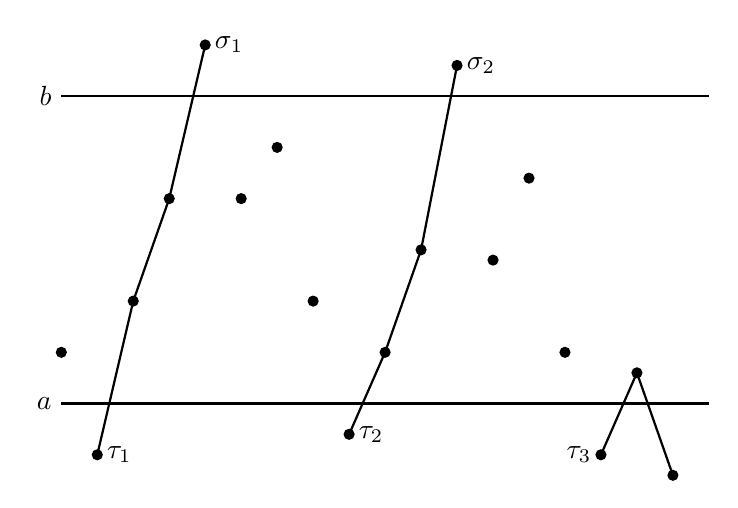
\begin{tikzpicture}
\begin{axis}[
scale = 1.6,
xmin = 0, xmax = 12,
ymin = 0, ymax = 7,
axis lines = none,
xtick = {0}, ytick = \empty,
clip = false,
]
\addplot[color=black, thick] coordinates{(2,1) (11,1)};
\addplot[color=black, thick] coordinates{(2,4) (11,4)};
\node [left] at (2,1) {$a$};
\node [left] at (2,4) {$b$};
\addplot[color=black, only marks, mark size=1.8pt] coordinates {(2,1.5) (2.5,0.5) (3,2) (3.5,3) (4,4.5) (4.5,3) (5,3.5) (5.5,2) (6,0.7) (6.5,1.5) (7,2.5) (7.5,4.3) (8,2.4) (8.5,3.2) (9,1.5) (9.5,0.5) (10,1.3) (10.5,0.3)};
\addplot[color=black, thick] coordinates{(2.5,0.5) (3,2) (3.5,3) (4,4.5)};
\node [right] at (2.5,0.5) {$\tau_1$};
\node [right] at (4,4.5) {$\sigma_1$};
\addplot[color=black, thick] coordinates{(6,0.7) (6.5,1.5) (7,2.5) (7.5,4.3)};
\node [right] at (6,0.7) {$\tau_2$};
\node [right] at (7.5,4.3) {$\sigma_2$};
\addplot[color=black, thick] coordinates{(9.5,0.5) (10,1.3) (10.5,0.3)};
\node [left] at (9.5,0.5) {$\tau_3$};
\end{axis}
\end{tikzpicture}
\end{center}
而下面的定理表明上穿数的期望存在一个上界.


\begin{theorem}[上穿不等式]
  如果$\{X_m:m\ge0\}$是一个下鞅, 那么
  $$(b-a)E(U_n)\leq E(X_n-a)^+-E(X_0-a)^+$$
\end{theorem}
\begin{proof}
  令$Y_m=a+(X_m-a)^+$, 根据推论\ref{cor:cor4.1}可知$\{Y_m\}$是一个下鞅, 显然它和$X_m$上穿$[a,b]$的次数相同. 易证
  $Y_{\sigma_i}-Y_{\tau_i}=Y_{\sigma_i}-a\ge b-a$对一切$i\le k$成立, 不难得到
  $$(H\cdot Y)_{\sigma_k}=\sum_{i=1}^{k}\sum_{j=\tau_i+1}^{\sigma_i}(Y_j-Y_{j-1})=\sum_{i=1}^{k}(Y_{\sigma_i}-Y_{\tau_i})\ge k(b-a)$$
  此外, 对于$\sigma_k\leq j\leq \tau_{k+1}$可得$(H\cdot Y)_j=(H\cdot Y)_{\sigma_k}$; 而对于$\tau_k<j\leq \tau_{k+1}$有$(H\cdot Y)_j\ge (H\cdot Y)_{\tau_k}=(H\cdot Y)_{\sigma_{k-1}}$, 由此得到
  $$(b-a)E(U_n)\leq (H\cdot Y)_n$$
  对一切$n\ge0$成立.

  最后令$K_m=1-H_m$, 易知$Y_n-Y_0=(H\cdot Y)_n+(K\cdot Y)_n$, 根据定理\ref{thm:thm4.6}可知$E[(K\cdot Y)_n]\geq E[(K\cdot Y)_0]=0$, 从而$E[(H\cdot Y)_n]\leq E(Y_n-Y_0)$, 这就得到了希望的结论.
\end{proof}

\begin{theorem}[鞅收敛定理]
  设$\{X_n\}$是一个下鞅, $\sup_n E(X_n^+)<\infty$, 那么当$n\to\infty$时, $X_n$几乎必然收敛于一个极限$X$, 并且$E|X|<\infty$.
\end{theorem}
\begin{proof}
定义
$$A=\left\{\omega: \liminf_{n\to\infty}X_n<\limsup_{n\to\infty}X_n\right\}$$
并且对于$a<b$定义
$$A(a,b)=\left\{\omega:\liminf_{n\to\infty}X_n<a<b<\limsup_{n\to\infty}X_n\right\}$$
于是取遍一切$a,b\in\mathbb{Q}$有$A=\cup A(a,b)$. 为了得出$\{X_n\}$的收敛, 只需证明对每个$a<b$有$P(A(a,b))=0$, 因为这意味着$P(A)=0$.

固定$a<b$, 设$U_n$为上穿数, 对于$\omega\in A(a,b)$, 当$n\to\infty$时有$U_n\to\infty$. 另一方面, 注意到$(X-a)^+\leq X^++|a|$, 由上穿不等式可知
$$E(U_n)\leq\frac{E(X_n^+)+|a|}{b-a}$$
再由$\sup_{n\ge1}E(X_n^+)<\infty$知$\sup_n E(U_n)<\infty$, 根据MCT可知
$$E\left(\limn U_n\right)=\limn E(U_n)$$
故而$$\limn U_n<\infty\quad\text{a.s.}$$这说明对一切$a<b$都有$P(A(a,b))=0$, 也即$\limn X_n=X$以概率1存在. 此外, Fatou引理保证了$E(X^+)\leq\liminf E(X_n^+)<\infty$, 于是
$$X<\infty\quad\text{a.s.}$$
为了看到$X>-\infty$, 注意到$\{X_n\}$是一个下鞅, 于是
$$E(X_n^-)=E(X_n^+)-E(X_n)\leq E(X_n^+)-E(X_0)$$
再由Fatou引理可知
$$E(X^-)\leq\liminf_{n\to\infty}E(X_n^-)\leq\sup_nE(X_n^+)-E(X_0)<\infty$$
这就完成了证明.

\end{proof}
\section{Doob不等式}
\begin{theorem}\label{thm:thm4.7}
  设$\{X_n\}$为一个下鞅, $N$为停时且$P(N\leq k)=1$, 那么$E(X_0)\leq E(X_N)\leq E(X_k)$.
\end{theorem}
\begin{proof}
  由于$\{X_{N\wedge n}\}$是一个下鞅, 故而
  $$E(X_0)=E(X_{N\wedge n})\leq E(X_{N\wedge k})=E(X_N)$$
  再令$K_n=1_{\{N<n\}}=1_{\{N\le n-1\}}$, 易知$\{K_n\}$是可料的, 由定理\ref{thm:thm4.6}可得$(K\cdot X)_n=X_n-X_{N\wedge n}$是一个下鞅, 并且
  $$E(X_k)-E(X_N)=E[(K\cdot X)_k]\geq E[(K\cdot X)_0]=0$$
  于是结论成立.
\end{proof}
\begin{theorem}[Doob极大不等式]
  设$\{X_n\}$为一个下鞅, $\overbar{X}_n=\max\{X_m^+: 0\leq m\leq n\}$, $\lambda>0$并且$A=\{\overbar{X}_n\geq \lambda\}$, 那么$\lambda P(A)\leq E(X_n1_A)\leq E(X_n^+)$.
\end{theorem}
\begin{proof}
  令$N=\inf\{m:X_m\ge\lambda\,\text{或}\,m=n\}$, 它是一个停时, 不难发现
  \begin{align*}
  A=\{\overbar{X}_n\ge\lambda\}&=\bigcup_{k=1}^n\{\overbar{X}_n\ge\lambda, N=k\} \\
  &=\bigcup_{k=1}^n\{X_N\ge\lambda, N=k\}=\{X_N\ge\lambda\}
  \end{align*}
  根据Markov不等式可知
  $$\lambda P(A)=\lambda P(X_N\ge\lambda)\leq E(X_N1_A)\leq E(X_n1_A)$$
  上式最后一个不等号是由定理\ref{thm:thm4.7}保证的, 而$E(X_n1_A)\leq E(X_n^+)$的证明是平凡的.
\end{proof}
\begin{example}[$\,$Kolmogorov极大不等式]
设$\xi_1,\xi_2,\cdots$为独立随机变量, $E(\xi_m)=0$且$\sigma_m^2=E(\xi_m^2)<\infty$, 于是$\{S_n^2\}$是一个下鞅, 再令$\lambda=x^2>0$, 根据Doob极大不等式可知
$$P\left(\max_{1\leq m\leq n}|S_m|\geq x\right)\leq x^{-2}\var(S_n)$$
\end{example}
\begin{theorem}[$L^p$极大不等式]
  如果$\{X_n\}$为一个下鞅, 那么对任意$1<p<\infty$都有
  $$E[(\overbar{X}_n^+)^p]\leq \left(\frac{p}{p-1}\right)^pE[(X_n^+)^p]\leq\infty$$
\end{theorem}
\begin{proof}
  如果$E(X_n^+)=\infty$, 那么结论是显然的, 故而假设$E(X_n^+)<\infty$. 显然, 对于任意$1<p<\infty$, $\varphi(x)=(x^+)^p$是$\R$上的一个不减的凸函数, 所以由定理\ref{thm:thm4.8}可知$\{(X_n^+)^p\}$也是下鞅, 从而对于一切$j\leq n$都有$E[(X_j^+)^p]\leq E[(X_n^+)^p]<\infty$. 又因为$(\overbar{X}_n^+)^p\leq \sum_{j=1}^{n}(X_j^+)^p$, 这意味着$E[(\overbar{X}_n^+)^p]<\infty$. 根据引理\ref{lem:lem2.2}可知
  $$E[(\overbar{X}_n^+)^p]=\int_{0}^{\infty}px^{p-1}P(\overbar{X}_n^+>x)\,\text{d}x=\int_{0}^{\infty}px^{p-1}P(\overbar{X}_n>x)\,\text{d}x$$
  根据Doob极大不等式可知, 对于一切$x>0$都有
  $$\lambda P(\overbar{X}_n\ge x)\leq E[X_n^+1_{(\overbar{X}_n\ge x)}]$$
  因此由Hölder不等式可得
  \begin{align*}
  E[(\overbar{X}_n^+)^p]&\leq\int_{0}^{\infty}px^{p-2}E[X_n^+1_{(\overbar{X}_n\ge x)}]\,\text{d}x \\
  &=\int_{0}^{\infty}px^{p-2}\int X_n^+1_{(\overbar{X}_n>x)}\,\text{d}P\text{d}x \\
  &=\frac{p}{p-1}E(X_n^+\overbar{X}_n^{p-1}) \\
  &\leq \left(\frac{p}{p-1}\right)E[(X_n^+)^p]^{1/p}E[(\overbar{X}_n^+)^{p}]^{1/q}
  \end{align*}
  其中$q=p/(p-1)$, 两端同时除以$E[(\overbar{X}_n^+)^{p}]^{1/q}$可知
  $$E[(\overbar{X}_n^+)^p]^{1/p}\leq\left(\frac{p}{p-1}\right)E[(X_n^+)^p]^{1/p}$$
  这就证明了结论.
\end{proof}

\begin{theorem}[$L^p$收敛定理]
  如果$\{X_n\}$是一个鞅, $\sup E|X_n|^p<\infty$, $p>1$, 那么$X_n\xrightarrow{a.s.} X$且$X_n\xrightarrow{L^p}X$.
\end{theorem}
\begin{proof}
  首先有$[E(X_n^+)]^p\leq (E|X_n|)^p\leq E|X_n|^p$, 根据鞅收敛定理可知$X_n\to X\,\text{a.s.}$, 再由$L^p$极大不等式得到
  $$E\left[\left(\sup_{0\leq m\leq n}|X_m|\right)^p\right]\leq\left(\frac{p}{p-1}\right)^pE|X_n|^p$$
  令$n\to\infty$, 再使用MCT可得$\sup |X_n|\in L^p$, 又因为$|X_n-X|^p\leq (2\sup|X_n|)^p$, 根据DCT可知$E|X_n-X|^p\to0$.
\end{proof}

\end{document} 